%%
% The BIThesis Template for Graduate Thesis
%
% Copyright 2020-2023 Yang Yating, BITNP
%
% This work may be distributed and/or modified under the
% conditions of the LaTeX Project Public License, either version 1.3
% of this license or (at your option) any later version.
% The latest version of this license is in
%   http://www.latex-project.org/lppl.txt
% and version 1.3 or later is part of all distributions of LaTeX
% version 2005/12/01 or later.
%
% This work has the LPPL maintenance status `maintained'.
%
% The Current Maintainer of this work is Feng Kaiyu.
%
% Compile with: xelatex -> biber -> xelatex -> xelatex

% !TeX program = xelatex
% !BIB program = biber

% 硕士论文模板 type=master
% 博士论文模板 type=doctor
% 开启盲审格式 blindPeerReview=true (如:[type=master,blindPeerReview=true])
% 开启双面打印 twoside=true (如:[type=master,twoside=true])
%
% 在 Linux 和 macOS 系统下,由于版权问题,中文字体和 Windows 系统下的字体不同。
% 如果想要获得与 Word 文档相同的效果,你有两个选择:
% 1. 使用 Windows 系统编译最终的论文。
% 2. 自己手动安装中易字库并添加选项:`\documentclass[...,ctex={fontset=windows}]{bithesis}`。
%
% **更多使用说明请参考 bithesis.pdf **

\documentclass[type=master,twoside]{bithesis}

\BITSetup{
  cover = {
    %% 使用以下参数来自定义封面日期
    date = 2023年6月,
    autoWidthPadding = 0.25em,
  },
  info = {
    % 想要删除某项封面信息,直接删除该项即可。
    % 想要让某项封面信息留空(但是保留下划线),请设置为空字符串。
    % 如需要换行,则用 “\\” 符号分割。
    classification = TQ028.1,
    UDC = 540,
    title = 面向非平整表面的缺陷检测算法研究,
    % 如需覆盖竖排标题,请配置以下选项。
    % 下面的例子展示了如何在竖排标题中使用垂直或者旋转的英文。
    % verticalTitle = {形状记忆聚氨酯{L } {T } {X }的合成 \rotatebox[origin=c]{-90}{Feng Kaiyu} 及其在织物中的应用},
    titleEn = Defect Detection Algorithm for Non-flat Surface,
    author = 雷勇,
    major = 控制科学与工程,
    school = 自动化学院,
    degree = 工学硕士,
    chairman = 费庆高工,
    defenseDate = 2023年6月1日,
    supervisor = 马宏宾教授,
    authorEn = Yong Lei,
    schoolEn = Automation ,
    supervisorEn = Prof. Si Li,
    chairmanEn = Prof. Wang Wu,
    degreeEn = Master of Philosophy,
    majorEn = Materials Science and Engineering, 
    defenseDateEn = {June, 12th, 2023},
    keywords = {缺陷检测;无监督;3D视觉;联邦学习},
    keywordsEn = Defect Detection; Unsupervised; 3D Computer Vision;Federated Learning,
    % 必要时置于封面右上角,并按照国家规定进行标记。
    % classifiedLevel = 密级\BigStar 保密期限,
  },
  % 在目录页中不显示摘要和主要符号对照表的标题。
  TOC = {
    abstract = false,
    abstractEn = false,
    symbols = false,
  },
  style = {
    pageVerticalAlign = scattered,
  },
  publications = {
    % 以下两个选项将影响「攻读学位期间发表论文与研究成果清单」中名称列表的省略阈值。
    % 一般来说,如果你在全部文献中最低排在第四位,建议你将两个值都设置为 4。
    % 更详细的说明请见手册。
    maxbibnames = 3,
    minbibnames = 1,
  },
  % 采用章节标题级别的附录格式
  appendices / chapterLevel = true,
}

\usepackage[
  defernumbers=true,
  backend=biber,
  style=gb7714-2015,
  gbalign=gb7714-2015,
  gbnamefmt=lowercase,
  gbpub=false,
  gbannote=true,
  gbpunctin=false,
  doi=false,
  url=false,
  eprint=false,
  isbn=false,
]{biblatex}

% 添加参考文献
\addbibresource{reference/main.bib}
% 攻读学位期间发表论文与研究成果清单,详细使用方法见 `chapters/pub.tex`。
\addbibresource{reference/pub.bib}


\usepackage{graphicx}

\usepackage{subfigure}
\usepackage{algpseudocode}
\usepackage[linesnumbered, ruled, lined,boxed,commentsnumbered]{algorithm2e}[1]
\usepackage{amssymb}
\renewcommand{\algorithmcfname}{算法}  %<---细节与重点
\SetKwInput{KwIn}{输入}  %<---细节与重点
\SetKwInput{KwOut}{输出}  %<---细节与重点
\usepackage{amsmath}
\numberwithin{equation}{section}
\usepackage{unicode-math}

\begin{document}

% 封面绘制
\MakeCover

% 打印书脊
\MakePaperBack

% 中文信息与英文信息
\MakeTitle

% 论文原创性声明和使用授权
\MakeOriginality

%%%%%%%%%%%%%%%%%%%%%%%%%%%%%%
%% 前置部分
%%%%%%%%%%%%%%%%%%%%%%%%%%%%%%
\frontmatter

% 摘要
%%
% The BIThesis Template for Graduate Thesis
%
% Copyright 2020-2023 Yang Yating, BITNP
%
% This work may be distributed and/or modified under the
% conditions of the LaTeX Project Public License, either version 1.3
% of this license or (at your option) any later version.
% The latest version of this license is in
%   http://www.latex-project.org/lppl.txt
% and version 1.3 or later is part of all distributions of LaTeX
% version 2005/12/01 or later.
%
% This work has the LPPL maintenance status `maintained'.
%
% The Current Maintainer of this work is Feng Kaiyu.

\begin{abstract}
  工业缺陷检测智能化是实现中国制造2025的重要内容之一,其中很多工业产品结构复杂、质检难度大,而目前缺陷检测算法主要是基于二维RGB图像,其在纹理、颜色等缺陷上表现优异,但在面对非平整表面这类复杂结构缺陷上仍有较大提升空间。此外,工业缺陷检测还存在缺陷未知且样本难以获取、企业对样本数据保密等不利于采用有监督深度学习进行缺陷检测的现实情况。因此,针对这些工业实际背景,本文首先搭建了实验平台,然后面向非平整表面提出了基于三维点云和多模态数据的少样本且缺陷未知的检测算法,并在最后应用联邦学习实现了分布式缺陷检测。

% 本文利用协作机器人挂载结构光相机搭建了硬件实验平台并开发了具有交互界面的自动数据采集应用,可以一键采集生成标准数据集,提高了后续缺陷检测算法的实验效率。

针对二维图像在结构缺陷检测不佳的场景,本文提出了基于三维点云数据的缺陷检测算法PillarCore。本文方法通过引入面向点云数据的局部特征描述子RoPS作为缺陷检测骨干网络输入端的特征提取器,将应用于二维缺陷检测的无监督算法里的存储体机制迁移到三维数据,利用训练时维护正常样本特征存储体并在测试时比较测试样本特征与存储体的正常样本特征的距离来判断测试样本是否有缺陷,从而实现未知缺陷检测。自建数据集和公开数据集的实验均表明PillarCore在面向非平整表面的缺陷检测上性能有明显提升。

针对纹理和结构缺陷共存的场景,本文提出了基于RGB-D的多模态缺陷检测算法HF-AST。该方法基于异构教师学生网络框架,假设仅在正常样本上训练的教师网络和学生网络在未知缺陷样本上有较大差异。本文通过将在大型数据集上预训练的网络作为RGB图像特征提取器,引入HOG算子作为深度特征提取器并在学生网络新增用于深度特征提取的卷积层,从而更好地融合深度信息。塑料件数据集的实验表明,相较于改进前的方法,HF-AST在多模态未知缺陷检测性能上有明显提升。

针对企业对数据集的保密和对缺陷检测算法分布式可扩展的需求,本文提出了基于联邦学习和异构教师学生网络的分布式缺陷检测算法。通过结构相对简单的学生网络回归仅在本地数据集上训练更新的复杂教师网络,该方法降低模型参数上传服务器进行全局聚合优化的传输负载。多类数据集模拟分布多产线的实验结果表明本文的分布式方法具有良好的扩展性。
\end{abstract}

\begin{abstractEn}
  Industrial defect detection intelligence is one of the important contents to achieve China Manufacturing 2025. Many industrial products have complex structures and are difficult to inspect. Currently, defect detection algorithms are mainly based on 2D RGB images, which perform well in texture and color defects. However, there is still much room for improvement when facing complex structural defects on non-flat surfaces. In addition, industrial defect detection also faces challenges such as unknown defects, difficulty in obtaining samples, and enterprises' confidentiality of sample data, which make it difficult to use supervised deep learning for defect detection. Therefore, this thesis first builds an experimental platform and then proposes a few-shot and unknown defect detection algorithm based on 3D point clouds and multimodal data for non-flat surfaces. Finally, this thesis also applies federated learning to industrial defect detection algorithms to achieve distributed deployment.

  To address the poor performance of 2D images in structural defect detection, this thesis proposes a defect detection algorithm based on three-dimensional point cloud data called PillarCore. This method introduces the RoPS local feature descriptor for point cloud data as the feature extractor at the input end of the defect detection backbone network. The storage mechanism used in unsupervised algorithms for 2D defect detection is migrated to 3D data. During training, the normal sample feature storage is maintained, and during testing, the distance between the test sample feature and the normal sample feature storage is compared to determine whether the test sample has a defect, achieving unknown defect detection. Experiments on self-built datasets and public datasets show that PillarCore has significantly improved performance in defect detection for non-flat surfaces.
  
  To address the coexistence of texture and structural defects, this thesis proposes a multimodal defect detection algorithm based on RGB-D called HF-AST. This method is based on a heterogeneous teacher-student network framework, assuming that the teacher network and student network trained only on normal samples have significant differences on unknown defect samples. This thesis uses a network pre-trained on a large dataset as an RGB image feature extractor, introduces the HOG operator as a depth feature extractor, and adds convolutional layers for depth feature extraction to the student network to better fuse depth information. Experiments on a plastic parts dataset show that compared to the improved method, HF-AST has significantly improved performance in multimodal unknown defect detection.
  
  To meet the needs of enterprises for data confidentiality and distributed scalable defect detection algorithms, this thesis proposes a distributed defect detection algorithm based on federated learning and a heterogeneous teacher-student network. By using a simple student network to update the complex teacher network only trained on local datasets, this method reduces the transmission load of model parameters uploaded to the server for global aggregation optimization. The experimental results of simulating multiple production lines with multiple datasets show that the distributed method proposed in this thesis has good scalability.
\end{abstractEn}


% 制作目录
\MakeTOC

% 插图目录
\listoffigures
% 表格目录
\listoftables

% 主要符号对照表
\input{./misc/0_symbols.tex}

\mainmatter

% 请根据论文内容,按照顺序添加章节。
%%
% The BIThesis Template for Graduate Thesis
%
% Copyright 2020-2023 Yang Yating, BITNP
%
% This work may be distributed and/or modified under the
% conditions of the LaTeX Project Public License, either version 1.3
% of this license or (at your option) any later version.
% The latest version of this license is in
%   http://www.latex-project.org/lppl.txt
% and version 1.3 or later is part of all distributions of LaTeX
% version 2005/12/01 or later.
%
% This work has the LPPL maintenance status `maintained'.
%
% The Current Maintainer of this work is Feng Kaiyu.

\chapter{绪论}

\section{本论文研究的目的和意义}
工业制品是现代社会中不可或缺的一部分,随着人们日益增长的美好生活需求,对工业制品品质的要求也越来越高,工业缺陷检测作为保障产品质量、维持生产稳定的重要技术之一,得到了越来越多的关注和重视。工业缺陷检测是指发现各种工业制品的外观可见缺陷,这些缺陷虽然微小,但可能严重危害产品的正常功能。工业制品的缺陷主要发生在产品的生产阶段,在以往的缺陷检测中,需要人工筛查,成本高、效率低,难以满足大规模质检需求。得益于工业成像、计算机视觉和深度学习等领域的不断创新,基于视觉的工业缺陷检测技术也得到了长足的发展,广泛应用于各个领域,为现代工业生产提供了更加高效、精准的质量保障手段。

基于视觉的工业缺陷检测技术高速发展的同时也面临着新的挑战和问题。对于诸如织物一类的平整表面,其表面几何结构通常不复杂,缺陷类别以纹理为主,针对这类问题的缺陷检测算法相对成熟且应用效果不错。但在工业实际问题中,需要质量检测的产品很少是平整的表面,大部分是曲率复杂、表面非平整的复杂几何结构,而针对此问题的相关研究较少,且应用于平整表面的缺陷算法也难以适用。因此,作为智能制造领域重要的基础研究与技术之一,面向非平整表面的工业缺陷检测技术不仅具有非常重要的研究价值,同时也拥有广阔的应用前景。

目前大部分缺陷检测的方法仅关注于单一的 RGB、灰度图像或其他成像形式的输入,这些输入在纹理类别上表现优秀,但其在几何结构类上任然有很大提升空间。因此在工业上,利用不同成像条件的差异产生区分力是一个正在探索的方向。比如在工业实际场景下,通过结构光、激光等方式获得的 3D 数据能进一步提升产品结构性缺陷的表达能力。

工业缺陷检测的另一个挑战是实际工况中常常面临只有正常样本,不易获取含有缺陷的样本。这使得产品的缺陷具有未知性与无规则性, 基于缺陷先验知识的方法存在较大的局限性。

因此本文针对工业实际痛点和需求,开展面向缺陷未知非平整表面的缺陷检测问题的研究实践。本文整体采用无监督的方法(即仅有正常样本),聚焦于利用几何结构表达能力更强的3D数据来进行缺陷检测,旨在解决缺陷未知条件下,面向非平整表面缺陷检测中复杂几何结构带来的问题,提升工业缺陷检测的性能。此外,为了综合不同成像条件的感知能力来应对更复杂的场景, 本文还通过融合多模态数据的特征来增强缺陷检测性能。

\section{国内外研究现状及发展趋势}
缺陷检测作为保证工业产品质量的重要环节,在工业领域具有广泛的应用。近年来,随着计算机视觉技术和深度学习的发展,基于视觉的非接触缺陷检测研究得到了国内外学者的广泛关注。本小节将从未知缺陷检测算法、特征提取算法和联邦学习算法三个方面出发介绍国内外研究现状及发展趋势。


\subsection{基于深度学习的未知缺陷检测研究}
目前基于计算机视觉,包括二维和三维图像,深度学习的缺陷检测方法主要是采用无监督的方式,即输入的训练数据仅为正常样本,模型在未标注的数据上训练,获取正常样本的内在特征和联系,缺陷被定义为正常范围之外的模式。无监督方法可以分为基于图像相似度的方法与基于特征相似度的方法。\cite{bergmannMVTec3DADDataset2022,chenSurfaceDefectDetection2021,zhengBenchmarkingUnsupervisedAnomaly2022,TaoXianJiYuShenDuXueXiDeBiaoMianQueXianJianCeFangFaZongShu2021a,luoGongyequexianjianceshenduxuexifangfazongshu2022}

\subsubsection{基于图像相似度}

基于图像相似度的方法在图像像素层面进行比较。其核心思想是重建出与输入样本最相近的正常图像,两者仅在缺陷区域存在差别。因此,生成图与输入图像的差异图可表示缺陷存在的概率,既可以用于判断整图是否包含异常,也可以设定阈值来得到缺陷的分割结果。此类方法常使用自编码模型与生成式模型,包括自编码器 (auto-encoder, AE)\cite{hintonAutoencodersMinimumDescription1993}、变分自编码器 (variational auto-encoder, VAE)\cite{kingmaAutoEncodingVariationalBayes2022}、生成对抗模型 (generative adversarial networks, GAN)\cite{hoGenerativeAdversarialImitation2016} 等。根据模型优化目标的不同,可分为基于图像重建的方法与基于图像恢复的方法。

基于图像重建的方法假设只在正常样本上训练模型,并使其学习足够好的分布特征来重建正常样本,那么模型应该只能较好地重建正常样本,而在缺陷区域则会产生大量的重建误差。该方法的缺陷检测性能受重建图像的质量影响,通过提高重建质量使重建图像与输入图像在缺陷区域差异凸显是目前主流改进方向。

基于 AE 的方法采用编码器-解码器结构的网络,编码器将输入图像编码为隐空间变量 z,解码器则利用 z 重建图像。通过计算输入图像与重建图像的重建误差,可以实现缺陷定位。然而,AE 在重建时存在模糊的现象,容易在计算重建误差时误检成正常像素点。提升重建图像的质量和利用模糊效应,将输入图像风格化是后续工作改进的方向。

基于VAE的方法利用编码器将正常图像映射到隐空间的先验分布,从对应分布中随机采样得到变量z,再利用解码器将z映射回图像空间。该方法假设缺陷区域的编码不服从该先验分布,无法较好地重建缺陷区域,从而可根据重建误差实现缺陷定位。由于可以构建比AE更加可控的结构化的隐空间流形,VAE可以从隐空间分布的角度来学习正常样本主要的共性特征。

基于 GAN 的方法利用了其对分布建模的强大能力,相比 AE 和 VAE,GAN 能够生成更清晰、高质量的图像。GAN 由生成器 (G) 和判别器 (D) 组成,两者互相对抗进行优化,生成器将从隐空间采样的变量映射为尽可能接近监督样本的图像,判别器则对生成样本的真实性进行判断。基于 GAN 的方法假设,当训练集中均为正常样本时,模型只能学习到正常样本的分布,因此隐空间变量经过生成器后只能得到正常图像。可根据待测图像与重建图像的误差实现缺陷定位,同时也可根据判别器的判别结果实现缺陷的检出。

AnoGAN\cite{schleglUnsupervisedAnomalyDetection2017}是第一个将GAN引入缺陷检测的方法。其采用迭代优化思路,随机采样一个变量输入到已在正常样本上训练完的DCGAN\cite{radfordUnsupervisedRepresentationLearning2016}中,得到生成图像并计算重建误差。通过反向传播更新隐空间变量,以找到最相近的隐空间变量。若样本经过 n 次迭代后重建误差仍然较大,则判为异常。但此方法由于优化过程需要反复迭代,大幅增加了模型推理时间,缺乏实用性。对此,Eff-GAN\cite{zenatiEfficientGANBasedAnomaly2019} 和 f-AnoGAN\cite{schleglFAnoGANFastUnsupervised2019} 在 GAN 的基础上引入了编码器,提取图像特征,以指导生成器生成最匹配的图像。f-AnoGAN 采用了多阶段的训练方式,第一阶段在正常样本上训练 WGAN \cite{gulrajaniImprovedTrainingWasserstein2017},第二阶段训练编码器以生成与输入最接近的正常图像。Eff-GAN 则将生成器的结构倒置作为编码器,训练时根据重建损失和判别损失共同约束进行端到端的训练。得益于无需繁复的迭代过程,推理速度提升明显。为保证重建图像的一致性,Komoto等\cite{komotoConsistencyEnsuredBidirectional2020}提出了将BI-GAN\cite{donahueAdversarialFeatureLearning2017}的生成器用AE模型代替的方法,实现图像空间和隐空间双向映射,其编码器提取的特征即为图像在隐空间的最佳表达。

% 把AE或VAE与GAN结合框架是当下主流趋势。Baur等\cite{baurDeepAutoencodingModels2019}将VAE与GAN结合,利用重建误差分割缺陷区域。GANomaly\cite{akcayGANomalySemisupervisedAnomaly2019}增加对抗训练并引入额外编码器,提升重建一致性。Skip-GANomaly\cite{akcaySkipGANomalySkipConnected2019}借鉴U-Net结构,结合多尺度特征,提升检测能力。DAGAN\cite{tangAnomalyDetectionNeural2020}参考BEGAN\cite{berthelotBEGANBoundaryEquilibrium2017},将判别器改为AE结构,适用于小工业数据集。Zhou等\cite{zhouEncodingStructureTextureRelation2020}引入结构提取模块,强化结构与纹理关系,提升重建质量和缺陷定位判断。Bergmann等\cite{bergmannImprovingUnsupervisedDefect2019}使用结构相似性损失函数,提升检测复杂真实工业数据能力。

由于模型容量大且缺陷与正常区域的特征差别小,即使仅在正常样本上训练,模型仍然可能将未见过的缺陷完整重建,因此基于图像重建的方法并非完全可靠。目前主要有两种思路来解决这一问题:一种方法是对隐空间分布施加约束,使其只对正常样本具有良好表示。另一种方法是引入特征存储器 (Memory) 来存储正常特征。

改进 Memory 方法利用额外空间存储正常训练样本特征,使模型重建正常图像。推理时,待测图像样本特征与 Memory 中匹配,利用其重建可以保证重建图像不会包含缺陷。Gong 等\cite{gongMemorizingNormalityDetect2019}提出的 MemoryAE比直接存储图像更加灵活,且节约内存。 Memory 的结构与更新机制是后续工作改进的方向。

基于图像重建方法简单直观,无需复杂预处理,但其输入与输出难以对齐,鲁棒性不好,易出现像素级误检。其次,AE 等模型虽基于正常样本训练,仍可能泛化到缺陷,甚至退化成恒等映射而无法检测异常。MemoryAE 方法存储大量正常样本特征,虽然一定程度上解决了恒等映射问题,但也导致模型开销大且效率低。

% 基于图像恢复方法将缺陷视为噪声,图像恢复则是去噪过程。此类方法的核心思想是在正常图像上加入缺陷后,训练网络模型将其恢复为对应的原始图像。常用的模型包括 AE 和 U-Net 等。训练完成后,模型具有根据上下文消除缺陷的能力。测试阶段利用恢复图像和输入图像的重建误差进行缺陷分割。由于模型的输入与输出不对等,此类方法能一定程度上避免恒等映射的问题。但其要求人工缺陷设计接近真实分布且具多样性,避免过拟合。其性能受恢复图像对齐程度影响,在实际工业部署时难满足实时性要求,效率较低。

\subsubsection{基于特征相似度的方法}

基于图像相似度的方法直观且可解释,但现有方法难以实现理想的重建效果,可能出现未对齐或改变风格的情况,导致检测错误并限制性能。利用特征空间比较高维特征以实现更鲁棒的检测是另一个方向。深度神经网络的特征提取能力提供了区分性的特征嵌入,减少无关特征的干扰。CNN提取的特征包含局部感受野的信息,不需要非常严苛的空间对齐,同时增加了对噪声的容忍能力。

% 深度一类分类方法结合神经网络与传统分类方法,提取正常图像特征并构建分界面。传统方法在大数据集或高维数据中检测异常时存在局限,深度学习可以帮助从高维工业图像中提取区分特征。早期混合方法\cite{erfaniHighdimensionalLargescaleAnomaly2016}先用自编码器学习特征,再用OC-SVM构建分界面。Deep SVDD\cite{ruffDeepOneClassClassification2018}结合深度学习与SVDD,训练神经网络将正常样本映射到超球内,但方法的特征中心点需人为指定,可能存在模型退化等。可以通过优化特征提取来规避局限\cite{kitamuraExplainableAnomalyDetection2019}。利用自监督学习设计监督信息与代理任务可以提升分类性能。此类方法用于工业缺陷检测任务时,需要对工业数据进行针对性的设计,主要难点在于挖掘和优化区分性特征。

特征距离度量方法不需要优化分界面,直接与待测样本进行比较。因此,需要合适的特征表达。使用正样本训练的特征提取器无法学习缺陷的特征,导致模型无法区分。因此,研究者选择使用预训练模型来描述图像的特征。度量形式主要有两种:基于向量的距离和基于分布的距离。

一种直观的方法是将待测图像与最相似的正常模板进行比较。该方法使用具有区分力的特征提取网络将多个输入图像映射到特征空间,它们的特征仅在缺陷区域差别明显。Napoletano 等\cite{napoletanoAnomalyDetectionNanofibrous2018}对正常图像划分区域,使用预训练模型提取特征、降维与聚类等操作来构建正常字典,以处理具有多样性的正常图像。Cohen 等\cite{cohenSubImageAnomalyDetection2021}提出的 SPADE 方法使用 kNN 法检索与待测样本语义最相似的 k 个正常样本,最后采用特征金字塔匹配的方法进行多尺度特征对齐,从而提升了缺陷定位的鲁棒性。这种方法简单直接,分割性能良好而稳定,尤其适用于固定机位的工业检测场景。但是,其在大型复杂数据集上的应用受到存储开销和检索时间的限制。

基于深度统计模型的方法通过对正常样本的特征进行概率分布建模来减少开销。Rippel等\cite{rippelModelingDistributionNormal2021}使用预训练网络提取正常样本的多尺度特征,并将各个特征图分别建模为多元高斯分布。测试阶段使用待测样本特征向量与正常分布的马氏距离来度量样本是否存在缺陷。Dedard等\cite{defardPaDiMPatchDistribution2021}将多元高斯分布建模于图像块的粒度上,利用多层特征图对齐组成的超列来融合多尺度特征,使得其存储和检索开销都比SPADE\cite{cohenSubImageAnomalyDetection2021}少。此方法尽管能够检测结构缺陷,但泛化性不佳。Rudolph等\cite{rudolphSameSameDifferNet2021}使用归一化流(NF)\cite{rezendeVariationalInferenceNormalizing2016}模型提升灵活性。该方法使用预训练模型提取正常样本的特征,然后基于NF模块将正常样本的特征映射到潜在空间Z,使其服从高斯分布。该方法假设异常样本的特征在Z空间将不服从高斯分布所以似然较小,从而可以敏锐地检测出微弱的缺陷,且无额外的存储开销。

另一种思路是将同一测试图像映射到特征空间的不同方式。该方法假设将图像映射到正常区域的结果相似,而对缺陷区域的映射结果差别较大。Bergmann等人\cite{bergmannUninformedStudentsStudentTeacher2020}首次将教师-学生框架应用于缺陷检测中。他们将大型预训练网络的表征能力通过知识蒸馏的方式迁移到轻量的教师网络中,并仅在正常数据集上训练多个随机初始化的学生网络,以使它们和教师网络在正常样本上的表达一致。其假设学生网络与教师网络在缺陷样本的表达具有较大的回归误差,且同时多个学生网络之间对缺陷的表达存在较大的不确定性,从而实现像素级的缺陷分割。为了解决感受野固定的问题,Salehi等人\cite{salehiMultiresolutionKnowledgeDistillation2021}直接将大型预训练模型作为教师网络,使用轻量紧凑的学生网络,以提升推理速度并专注于区分性特征。使用模型解释性方法,如SmoothGrad\cite{smilkovSmoothGradRemovingNoise2017}等,使模型可以适应多种尺度的缺陷,并极大地降低了计算复杂度,实现了实时检测。Gudovskiy等人\cite{gudovskiyCFLOWADRealTimeUnsupervised2022}提出了一种基于一个条件归一化流框架的实时无监督缺陷检测模型CFLOW-AD ,其包括一个经过鉴别预训练的编码器,以及一个多尺度生成解码器,后者明确地估计编码特征的可能性。

\subsubsection{3D缺陷检测}

相比于大量关于2D异常检测方法的研究,3D缺陷检测相关研究相对较少,是未来发展的趋势。3D缺陷检测较早的工作是研究者在医学成像研究中将缺陷检测方法应用到体素数据中。Simarro等人\cite{simarrovianaUnsupervised3DBrain2021}将应用于2D图像的f-Anogan\cite{schleglFAnoGANFastUnsupervised2019}扩展到3D。Bengs等人\cite{bengsThreedimensionalDeepLearning2021}提出了一种针对医学体素数据的3D自编码器方法,其空间消除方法可进一步提高缺陷检测性能并减少对大型数据集的要求。

然而体素数据与点云3D数据仍然有较大差异,Bergmann等人\cite{bergmannMVTec3DADDataset2022}认识到缺乏用于3D点云数据异常分割的数据集,推出了MVTec 3D-AD,为3D缺陷检测算法的研究打开了新局面。在该数据集上,Bergmann和Sattlegger \cite{bergmannAnomalyDetection3D2023}将教师学生网络扩展到3D点云缺陷检测,称为$3D-ST_{128}$。Horwitz等人\cite{horwitzBackFeatureClassical2022}将2D图像的PatchCore方法扩展到3D,其使用FPFH作为3D特征提取和预训练的网络作为RGB图像特征提取。此外,其做了多项对比实验证明加入3D数据确实有利于提升缺陷检测性能且使用简单的3D特征提取描述子即可取得不错效果。Rudolph等人\cite{rudolphAsymmetricStudentTeacherNetworks2022}提出异构的教师学生网络AST,教师网络使用标准化流而学生网络使用简单残差网络,其假设教师模型在正常样本上训练,学生通过回归教师网络模型,两者在缺陷样本上将会有较大差异,从而实现缺陷检测。AST网络利用EfficientNet提取二维图像特征作为输入,深度图像只混合原始深度信息以达到和二维特征图匹配。实验表明,AST在多模态缺陷检测上性能优异。

% \subsubsection{自监督}

% 自监督学习属于无监督学习的一种。其利用无标注数据自动设计监督标签,并通过类似有监督学习的方式训练模型。主要可以分为三种方法:基于图像复原、基于缺陷合成和基于图像变换的方法。

% 基于图像复原的方法可以挖掘图像内在属性与内容的关联性。其主要思想是显式地训练模型,将经过变换的输入图像复原为原始正常图像。在测试阶段,正常区域的像素基本不变,而异常区域被擦除,进而根据重建误差实现缺陷的检测与分割。这类方法展现出更强的泛化性,但在测试时需要遍历图像的预处理过程,影响了模型的效率。

% 基于缺陷合成的方法可以在正常图像上构造缺陷,得到缺陷样本及其图像或像素级精确的标签。然后可以利用对比学习或有监督的方式训练模型。测试时,分别在图像与图像块维度进行高斯密度估计,以实现缺陷的检测与定位。然而,缺陷合成的方法对于合成方式非常敏感,往往容易过拟合到人造缺陷模式上。

% 基于图像变换的方法,通过代理任务训练判别式模型。该方法假设模型能够正确判别正常样本的变换方式,而无法预测异常样本的变换方式。这类方法往往会与深度一类分类方法结合。常见的变换方式包括旋转角度、颜色变化、顺序打乱等,将变换的编号或参数作为监督信息,训练网络预测正常图像的变换方式。然而,由于图像变换往往是全局的,此类方法通常用于图像级的缺陷检测。


\subsection{特征提取的研究}
针对RGB图像的特征提取方法主要分为传统方法和基于学习的方法。\cite{chenSurfaceDefectDetection2021}传统特征提取方法主要有基于纹理特征的方法、基于颜色特征的方法和基于形状特征的方法三类方法。

纹理特征反映了图像的同质性现象,基于纹理特征的方法包括通过直方图、灰度共生矩阵等特征描述灰度值的空间分布的统计方法、利用傅里叶变换和小波变换等的信号处理方法和对图像建模来描述纹理特征的模型方法。颜色特征计算量小,不受图像大小、方向、视角等因素影响,具有高鲁棒性。基于颜色特征的方法有表示图像中不同颜色比例的颜色直方图、使用矩阵表示颜色分布的颜色矩和改进颜色直方图算法的颜色相干向量。基于形状的方法可以用于目标检索,其中轮廓法通过霍夫变换和傅里叶形状描述子来获得图像的形状参数,前者利用图像的全局特征将边缘像素连接起来形成闭合边界,后者则利用对象边界的傅里叶变换作为形状描述,将二维问题转化为一维问题。

Lowe等人\cite{loweDistinctiveImageFeatures2004}提出了具有旋转、尺度和平移不变性的SIFT,其在图像中识别关键点或兴趣点,通过旋转将最显著的方向与基本方向对齐来减少旋转歧义,从而实现在旋转图像之间进行匹配。

Dalal等人\cite{dalalHistogramsOrientedGradients2005}提出了一种特征描述子HOG(Histograms of Oriented Gradients),其与SIFT等局部图像描述符类似,但是计算方式不同,可以更有效地进行密集采样。HOG通过将图像分成称为单元格的小连通区域,并计算每个单元格内像素的梯度方向或边缘方向的直方图。 

基于学习的方法通常使用在大型数据集上预训练的神经网络模型来提取图像的特征图。He等人\cite{heDeepResidualLearning2016}提出了可用于图像分类任务的ResNet,其过跳过连接将一个层的输出添加到不一定相邻的另一个层中来学习残差函数,解决了梯度消失问题,是网络可以变得深层。

Tan等人\cite{tanEfficientNetRethinkingModel}提出了基于一种简单但高效的复合缩放方法的EfficientNet,并通过神经架构搜索设计了一个新的基线网络,将其扩展为一组模型,称为 EfficientNets。该方法使用一组固定缩放系数统一缩放深度、宽度、分辨率的所有维度,实验表明该方法在 MobileNets 和 ResNet 扩展上的有效性。

针对三维数据的特征提取方法主要有基于空间特征的方法和基于几何特征的方法。\cite{georgiouSurveyTraditionalDeep2020,guoNovelLocalSurface2015,guoComprehensivePerformanceEvaluation2016,hutchisonUniqueSignaturesHistograms2010,liu3DImagingAnalysis2020,rusuAligningPointCloud2008,rusuFastPointFeature2009,tombariCombinedTextureshapeDescriptor2011,yangEffectSpatialInformation2017,yangTOLDIEffectiveRobust2017,yulanguoRoPSLocalFeature2013,zhangNotAllPoints2022,zhaoHoPPFNovelLocal2020}基于空间特征的方法通过根据表面上的点的空间分布(例如坐标)生成直方图来表示局部表面。这种方法通常从为关键点构建局部参考框架(LRF)开始,并根据 LRF 将 3D 支持区域划分为多个区间。在每个空间区间中累积空间分布测量(例如点数)以生成局部表面的直方图。\cite{guoComprehensivePerformanceEvaluation2016}

Guo等人\cite{yulanguoRoPSLocalFeature2013}提出了一种基于旋转投影统计的3D特征描述符RoPS(Rotational Projection Statistics),其通过将相邻的3D点旋转投影到2D平面上,并计算这些平面上分布矩阵的低阶矩和熵来构建的,对噪声和网格分辨率的变化具有鲁棒性。

Guo等人\cite{guoNovelLocalSurface2015}还提出了一种能够在杂波和遮挡的情况下识别3D物体的局部特征描述子TriSI(Tri-Spin-Image),其通过生成三个签名来编码局部表面的几何信息,然后这些签名被连接起来形成原始的TriSI特征向量,并使用主成分分析(PCA)技术进一步压缩该特征。

基于基于几何特征的描述子通过根据表面上点的几何属性(例如法线,曲率)生成直方图来表示局部表面。

Rusu等人\cite{rusuAligningPointCloud2008}研究了使用PFH(Persistent Feature Histograms)来将点云数据视图对齐到一致的全局模型。给定一组嘈杂的点云,通过分析不同尺度下特征的持久性,估计一组描述每个点局部几何的稳健的多维特征。

Rusu等人\cite{rusuFastPointFeature2009}在点云配准的背景下,又提出了FPFH(Fast Point Feature Histograms),该方法通过计算其邻居的相对方向直方图来描述点云中一个点的局部几何特性。FPFH是PFH描述子的扩展,更具计算效率和噪声鲁棒性。





\subsection{联邦学习的研究}
随着近年来工业界对数据隐私及安全问题越来越重视,数据孤岛现象越来越多,而这与深度学习对大量训练数据的需求矛盾,制约了深度学习在工业缺陷检测的落地。联邦学习作为能够保护隐私、解决数据孤岛问题的一种分布式机器学习方法成为研究热点。\cite{banabilahFederatedLearningReview2022,liFederatedLearningChallenges2020,liuRecentAdvancesFederated2023,mammenFederatedLearningOpportunities2021}

联邦学习只在本地利用数据样本进行训练,不上传共享数据而是通过上传共享模型参数实现在多个分散设备或服务器上分布式学习,从而解决在大量分散数据上进行训练时面临的隐私和安全问题,确保数据隐私和安全性。

谷歌提出了联邦学习的概念,介绍了一种实用方法FedAvg\cite{mcmahanCommunicationEfficientLearningDeep2023},该方法允许用户共享经过训练的模型,而无需将数据集中存储。FedAvg将训练数据分布在移动设备上,并通过聚合本地计算的更新来学习共享模型。实验表明,FedAvg对于不平衡和非独立同分布数据具有鲁棒性。在五种不同的模型架构和四个数据集上进行了广泛的实证评估。

联邦学习可分为同构和异构两种类型,根据输入数据集、本地网络模型和设备类型。数据异构性可能导致本地节点处于不同情况下,从而导致各种数据分布。多任务学习可同时为多个相关任务学习模型,其核心设计原则是捕获任务之间的关系并促进学习过程。客户端的不同数据分布可以被视为一种多任务学习。

在FedAvg之后,联邦学习的研究主要有两个方向:解决客户端数据异构性的问题,设计联邦学习优化算法以加快模型收敛速度;解决联邦学习模型上传和下载中的通信成本高问题,设计提高通信效率的算法。此外,为了方便研究实验,还提出了一些联邦学习相关框架。\cite{zengFedLabFlexibleFederated2022}

目前联邦学习聚合优化主要有权重级聚合、特征级聚合和其它聚合\cite{sattlerRobustCommunicationEfficientFederated2019,wangFederatedLearningMatched2020,zhaoFederatedLearningNonIID2022}。FedAvg是典型的权重级聚合方法,Collins等人\cite{collinsFedAvgFineTuning2022}研究了FedAvg算法的泛化能力,其能够利用客户端数据分布的多样性学习客户端任务之间的共同数据表示,从而输出具有表示学习能力的模型。还证明了FedAvg在共享表示是线性映射的情况下仍能学习到泛化到新客户端的共享表示以及其在异构数据的联邦图像分类中的表示学习能力。

Wu等人\cite{banabilahFederatedLearningReview2022}介绍了一种名为FedKD的通信高效联邦学习方法。FedKD通过知识蒸馏有效地降低了通信成本。在FedKD中,客户端和服务器不直接传递大模型,而是提取了一个小学生模型和一个大教师模型。只有学生模型被共享和协同学习。每个客户端都维护一个本地教师模型和共享学生模型的本地副本,通过自适应知识蒸馏方法从本地数据和彼此提取的知识中学习。此过程将被迭代执行,直到学生模型收敛。为了降低学生模型更新时的通信成本,还提出了一种基于奇异值分解(SVD)的动态梯度近似方法来压缩通信梯度。

Han等人\cite{hanFedXUnsupervisedFederated2022}提出了一种无监督的联邦学习算法FedX,通过本地和全局两个层面上的独特的两面式知识蒸馏来学习数据表示。两面式知识蒸馏可以从本地数据中发现有意义的表示,同时通过使用全局知识消除偏见。FedX可以应用于现有算法,实验表明模型在五种无监督算法上显著提高了性能,并进一步提高训练速度。

在联邦学习通信与压缩方面\cite{linDefensiveQuantizationWhen2019,linDeepGradientCompression2020,reisizadehFedPAQCommunicationEfficientFederated2020,zhouCommunicationefficientFederatedLearning2023,zhouCommunicationefficientFederatedLearning2023},Haddadpour等人\cite{haddadpourFederatedLearningCompression2021}提出了采用周期性压缩(量化或稀疏化)通信的方法FedCOM,并分析其在同质和异质本地数据分布设置下的收敛性质。作者阐述了梯度压缩和周期性通信中本地计算的关系。FedCOM通过周期性平均、本地和全局学习速率以及压缩通信,在同质设置中比现有方法收敛更快。

在联邦学习框架方面,Zeng等人\cite{zengFedLabFlexibleFederated2022}等人提出了一种轻量级的开源联邦学习框架FedLab。该框架的设计侧重于FL算法的效率和通信效率,并且在不同的部署场景中具有可扩展性。该框架提供了FL模拟所需的必要模块,包括通信、压缩、模型优化、数据分区和其他功能模块。FedLab提供标准同步和异步FL系统的标准化FL实现方案以及FL数据集基准和标准FL模拟的功能模块,减轻了联邦学习社区中研究人员实现新方法的负担。


\section{论文研究内容与组织结构}
\subsection{论文研究内容}
本文面向工业缺陷检测中非平整表面的复杂产品,针对其缺陷样本匮乏、结构化缺陷检测性能有待提升的两个痛点,搭建视觉实验平台,采集点云数据和RGB-D多模态数据,分别研究仅利用正常样本数据实现工业缺陷检测的算法,并探索了将联邦学习应用到本文算法实现分布式缺陷检测。本文主要研究内容如下:

(1)搭建缺陷检测实验平台

实验平台是本文缺陷检测算法研究的基础。本文研究通过协作机器人和结构光激光相机组合搭建实验硬件平台,并设计了带有交互界面的自动数据采集应用,提供后需研究方法所需的标准数据集。除了数据采集平台,本文还搭建了缺陷算法运行测试的软件平台。

(2)研究基于3D点云数据的缺陷检测算法

非平整表面的工业产品结构非常复杂,其缺陷也主要以结构缺陷为主,二维图像适用的缺陷检测方法对此性能不佳,因此需要一种更加高效的方法来表征这种结构。本文旨在探讨如何利用点云数据来表征工业产品的结构。首先,本文对点云数据进行了合理的预处理,以提高点云的计算效率。接着,本文引入了一种基于空间的点云特征描述子RoPS,该描述子可以提取点云的特征。最后,本文使用Patchcore的骨干对提取的特征进行存储,从而实现对未知缺陷的检测。

(3)研究基于RGB-D数据的多模态缺陷检测算法

除了结构缺陷,有时非平整表面的工业产品也会有颜色和纹理等非结构的缺陷,单纯使用2D或3D数据都不足以满足需求。因此,本文采用一种多模态融合的方法来解决问题。首先,本文采集了RGB-D的多模态数据,然后分别利用预训练的模型提取RGB图像的特征和引入HOG提取深度图像的特征,从而可以更加全面地表征工业产品多种特征。接着,本文将这些特征与位置编码拼接,送入异构的教师学生网络训练模型来实现多模态的缺陷检测,其中学生网络通过新增深度特征卷积层来改进多模态融合。

(4)研究基于联邦学习的分布式缺陷检测算法

分布式缺陷检测检测是工业缺陷检测未来的发展趋势。本文研究将联邦学习应用到本文改进的异构教师学生缺陷检测算法上来实现分布式缺陷检测,并通过联邦学习仿真框架利用大型数据集模拟多个分布式产线,从而验证本文的有效性和探索其扩展性。

\subsection{论文组织结构}
\begin{figure}[htbp]
    \centering
    \includegraphics[width=0.75\textwidth]{figures/1/paper-framework.pdf}
    \caption{论文组织结构图}\label{fig:paper-framework}
  \end{figure}
本文面向非平整表面的缺陷检测算法研究从背景出发搭建实验平台,研究不同场景下缺陷检测算法并应用分布式方法部署算法,整个论文的组织结构如图\ref{fig:paper-framework}所示。

第一章绪论介绍了面向非平整表面缺陷检测的研究背景和意义,并对国内外未知缺陷检测算法、特征提取和联邦学习研究现状和发展趋势进行了总结,从而提出了基于3D点云数据和多模态数据两种场景下未知缺陷检测算法的研究以及应用分布式联邦学习的思路。最后概括介绍了本文的研究内容和组织结构。

第二章首先从搭建视觉缺陷检测系统的核心传感器结构光相机的原理出发,介绍了本文实验平台的硬件平台和软件平台并进行了相机标定。此外实验平台主要是采集数据集为本文算法验证提供支持,因此介绍了本文开发的具有交互界面的数据自动采集应用。最后介绍了用于实验中衡量缺陷检测算法性能的评价指标。

第三章首先介绍了基于3D点云数据的缺陷检测算法框架,然后介绍了对输入算法的点云数据进行预处理的滤波算法和将点云贪婪三角化的原理,接着介绍了本文引入的RoPS局部特征描述子的原理和缺陷检测骨干模型的原理。最后在第二章搭建的实验平台上开展了对比实验,证明了本文所提算法的有效性。

第四章研究了基于多模态的缺陷检测,同样从算法整体框架开始,然后介绍对输入多模态数据的预处理,利用预训练网络对RGB图像的特征提取原理和用HOG对深度图像的特征提取的原理,接着分别介绍了使用标准化流的教师网络和本文改进的深度特征融合学生网络。最后也在本文的实验平台上开展了对比实验,验证了本文改进算法对缺陷检测性能的提升。

第五章从联邦学习应用到异构教师学生网络的框架开始,介绍了联邦学习范式的理论基础,然后说明了本文使用的联邦学习全局聚合优化方法和通讯压缩方法的原理,接着介绍了联邦学习的仿真框架,并最后在该框架上进行了实验,证明了利用联邦学习实现缺陷检测算法分布式部署的可行性。

最后结论部分对本文的研究内容和创新点进行了总结和分析,并指出了本文研究中有待改进之处以及本文尚未深入探索的研究方向。
\chapter{实验平台}
\section{结构光相机原理}
3D表面成像的一个主要方法是基于结构光的使用,即通过特殊投影仪或由空间光调制器调制的光源对场景进行有源照明,生成具有空间变化的2D结构化照明。结构光图案上每个像素点的强度由数字信号表示。

使用成像传感器来获取受结构光照明下场景的二维图像。如果场景是一个没有任何三维表面变化的平面表面,则所获得图像中显示的模式类似于投影结构光模式。然而,当场景中的表面是非平整面时,从相机看到的投影结构光模式会被表面的几何形状扭曲。 结构光3D表面成像技术原理在于基于从投影结构光模式失真信息提取3D表面形状。可以使用各种结构光原理和算法计算出场景中物体的精确3D表面轮廓。成像传感器、结构光投影仪和物体表面点之间的几何关系如图\ref{fig:3d-camera}所示。\cite{gengStructuredlight3DSurface2011,salviStateArtStructured2010}


% 可以用三角测量原理表示,如式

% \begin{equation}
%   R=B \frac{\sin (\theta)}{\sin (\alpha+\theta)}
% \end{equation}

\begin{figure}[htbp]
  \centering
  \includegraphics[width=0.5\textwidth]{figures/2/3d-camera.pdf}
  \caption{结构光测距原理示意图}\label{fig:3d-camera}
\end{figure}

三角测量式三维成像的关键在于区分出二维投影获取的图像中的单个投射光斑。根据投射光源可将其分二值编码、彩色编码、光栅条纹编码等。其中,光栅条纹编码最常见,它具有高精度、快速等优势。\cite{vanderjeughtRealtimeStructuredLight2016}在使用光栅条纹技术的结构光相机进行高度测量时,通常先采取四步相移、多频外差等方法获取样本表面高度的绝对相位调制,然后基于三角测量原理进行计算。\cite{wangGuangzhajiegouguangxitongceliangwuchayunihejingduyanjiu2020}

相移法是一种用于三维表面成像的著名条纹投影方法。一组正弦波图案被投射到物体表面上。平面上任一像素位置处接收的光强$I_{n}(x, y)$可由式\ref{equ:in}表示

\begin{equation}\label{equ:in}
  I_{n}(x, y)=I_{mod}(x,y) \cos \left(\varphi(x, y)+\delta_{n}\right)+I_{0}(x,y)
\end{equation}


其中$I_{mod}(x,y)$是振幅,$\varphi(x, y)$是像素点的相位,$\delta_{n}$ 是每次拍摄时移动的相位,这个三个变量组成的$I_{mod}(x,y) \cos \left(\varphi(x, y)+\delta_{n}\right)$是系统投射的余弦调制光强(交流成分);$I_{0}(x,y)$是直流成分,即环境光强。根据N步相位法,$\delta_{n}=\frac{2 \pi(n-1)}{N}, n=1,2, \cdots, N$ ,而上式有三个未知量,因此N >= 3,即通过三幅或三幅以上投影可求解未知相位,相位计算公式如式\ref{equ:varphical}所示。

\begin{equation}\label{equ:varphical}
  \varphi(x, y)=\arctan \left(\frac{\sum_{n=1}^{N} I_{n}(x, y) \cos \left(\frac{2 n \pi}{N}\right)}{\sum_{n=1}^{N} I_{n}(x, y) \sin \left(\frac{2 n \pi}{N}\right)}\right)
\end{equation}


根据测量相位$\varphi(x, y)$和参考平面的相位值之间的差异按式\ref{equ:distance}可以计算出3D坐标。

\begin{equation}\label{equ:distance}
  h=\frac{L \times x_{A C}}{d+x_{A C}}=\frac{L \times P_{0} \times \varphi_{A C}}{2 \pi d+P_{0} \times \varphi_{A C}}
\end{equation}


其中L表示系统与基准平面的距离,d表示相机与投影仪之前的基线距离,$P_{0}$ 表示投影光栅条纹的周期, $\varphi_{A C}$为相位差。




\section{硬件平台}

实验硬件平台主要包括结构光相机、协作机器人、工控机和GPU服务器。结构光相机用于采集样本,是视觉方案中最重要的提供输入的传感器。协作机器人用于挂载结构光相机执行运动指令。工控机用于运行自动数据采集程序。GPU服务器负责对采集数据进行处理并进行缺陷检测输出结果。

\subsection{传感器设备}
\begin{figure}[htbp]
  \centering
  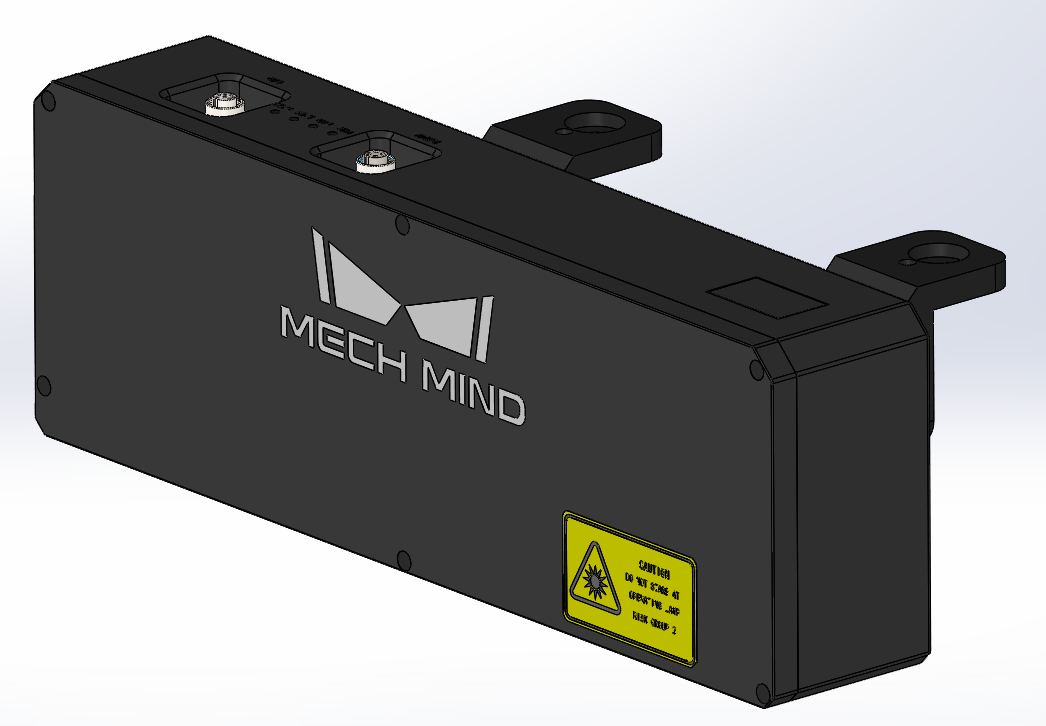
\includegraphics[width=0.5\textwidth]{figures/2/Mech-Eye-V3.png}
  \caption{梅卡曼德Mech-Eye PRO M 工业级3D相机}\label{fig:Mech-Eye-V3}
\end{figure}
本文采用梅卡曼德的PRO M高性能工业级3D相机作为视觉传感器搭建系统,如图\ref{fig:Mech-Eye-V3}所示。该相机使用蓝光作为结构光光源,能够采集被检物体表面的深度信息以及RGB色彩信息,可以直接输出ply格式的无序点云数据、具有RGB通道的彩色图像和tiff格式的单通道深度图像。此外,该相机具有精度高,速度快,抗环境光性能优异,运行稳定的优点,其部分参数如表\ref{tab:category}所示。其中1m到2m的推荐工作距离与AUBO-E5协作机器人的工作区域匹配,能覆盖本文实验所用的工业产品;1920 × 1200的分辨率和2.3MP的像素数表示其能输出高清晰度的RGB图像;0.2mm @ 2m的Z向单点重复精度则表示其能提供高精度的深度图。
\begin{table}[htbp]
  \centering
  \caption{结构光相机部分重要参数} \label{tab:category}
  \begin{tabular*}{0.75\textwidth}{@{\extracolsep{\fill}}cccc}
  \toprule
    指标			&参数		 \\
  \midrule
    工作距离范围$(mm)$ &  $1000\sim 2000$    \\
    分辨率			&$1920\times 1200$		 \\
    像素数$(MP)$	&$2.3$	 \\
    Z向单点重复精度$(\sigma)$	& $0.05mm @ 1m$\\
    典型采集时间$(s)$	& $0.6\sim0.9$\\
    基线长度$(mm)$ &  $68$    \\
    光源$(mm)$ &  蓝光LED$(459nm,RG2)$    \\
  \bottomrule
  \end{tabular*}
\end{table}


\subsection{协作机器人}

本文使用AUBO-E5协作机器人挂载结构光相机,并接收工控机自动数据采集程序的指令进行运动,实现智能化采集大量多视角的样本数据,为后续缺陷检测任务服务。AUBO-E5协作机器人由机械臂、控制柜和示教器共同组成。机械臂具有6自由度,能够负载5kg,其臂展有1008mm,最大工作半径886.5mm,重定位精度达到0.02mm,能够满足在实验室中轻量化作业需求。示教器作为人机交互工具,具有显示器,提供可视化界面操作机械臂。协作机器人如图\ref{fig:aubo}所示,左图为机械臂,右图为示教器。
\begin{figure}[htbp]
  \centering
  \begin{subfigure}
      \centering
      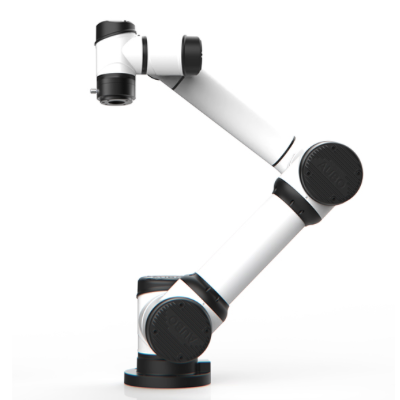
\includegraphics[width=.35\linewidth]{figures/2/aubo-1.png}  
    \end{subfigure}
    \begin{subfigure}
      \centering
      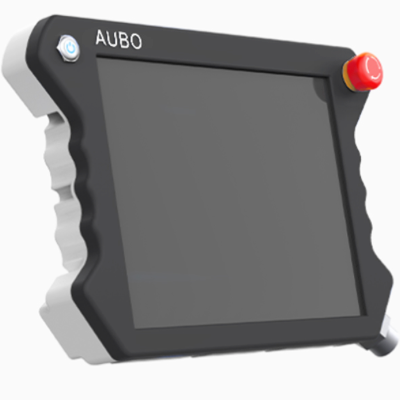
\includegraphics[width=.35\linewidth]{figures/2/aubo-2.png} 
    \end{subfigure}
  \caption{AUBO-E5协作机器人}
  \label{fig:aubo}
\end{figure}



\subsection{计算单元}
本文使用的运行缺陷检测算法程序服务器硬件上搭载了英伟达RTX3090型号的GPU,具有10496个CUDA核以及24GB的GDDR6X类型显存;CPU使用的是AMD EPYC 74F3,具有24核48线程,基础频率3.2GHz。

\begin{figure}[htbp]
  \centering
  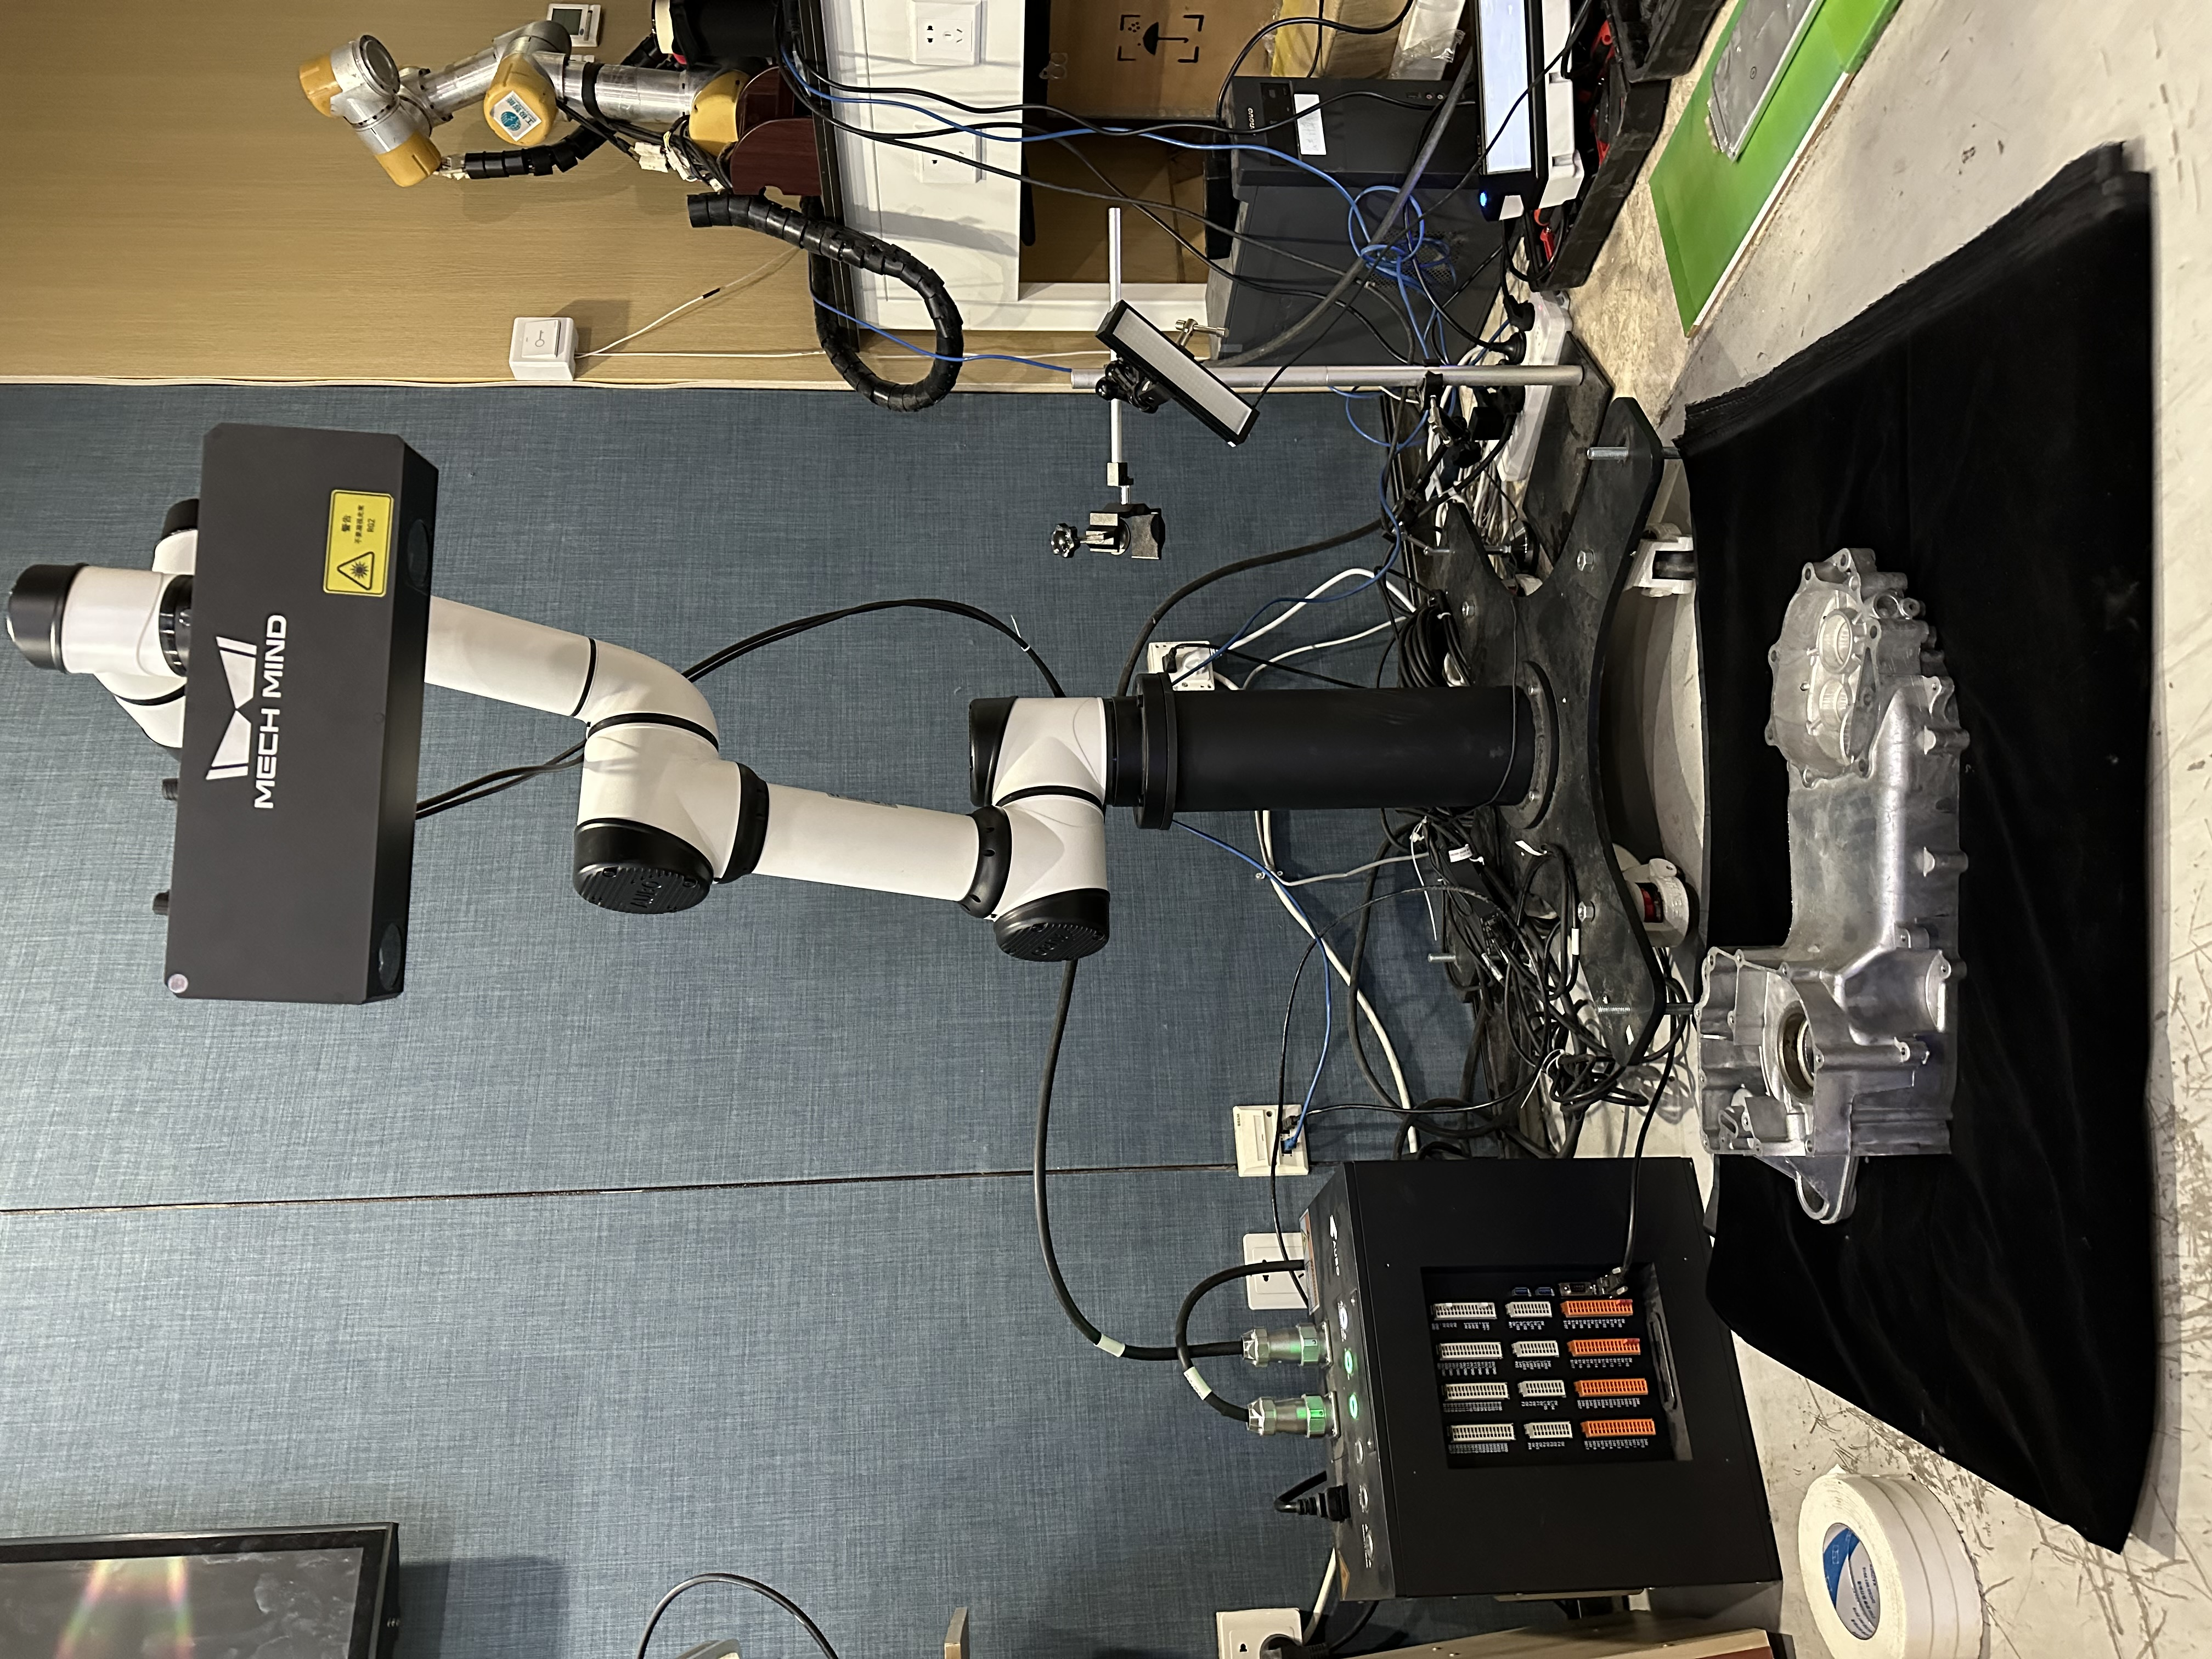
\includegraphics[width=0.5\textwidth,angle=270]{figures/2/hw-platform.jpeg}
  \caption{缺陷检测实验硬件平台}\label{fig:hw-platform}
\end{figure}
本文在实验室组合以上硬件设备搭建的实验硬件平台如图\ref{fig:hw-platform}所示,环境光源为室内灯光,存在直射光源干扰。实验平台的感知系统由协作机器人、结构光相机和模拟工作台共同组成,采集指令和采集数据存储由工控机处理。实验平台的设计目标是自动化采集样本数据,实现仅依靠正常样本的缺陷检测。本文的实验对象为工作区内的工业产品,针对不同场景,本文采集不同的数据并使用不同方法进行处理,实现被检物的缺陷检测。


\section{软件平台}
本文使用的工控机系统环境为Ubuntu18.04,主要使用的库包括GUI库Qt、点云处理库PCL和Open3D、外设SDK(相机和机械臂)和深度学习训练框架Pytorch等。

Qt是一个跨平台的C++应用程序开发框架,可以用来开发GUI程序。在本文的人机交互界面中,我们使用了Qt Creator IDE进行开发,该IDE提供了可视化编辑UI界面的功能。

PCL(Point Cloud Library)和Open3D都是点云处理库,PCL是基于C++11标准的模块化库,Open3D是基于Python的模块化库。两者都可以对点云数据进行读取、可视化以及滤波,针对特征提取等高阶用法,两者提供的方法有所区别。由于Open3D基于Python,其对深度学习模型的支持较好,适合在模型训练阶段快速试验;而PCL基于采用C++,对于大量数据处理其优势显现,因此本文根据实际阶段应用两者。

PyTorch是一个开源的深度学习框架,使用动态计算图,方便灵活调试。此外,Pytorch可以利用NVIDIA的CUDA和cuDNN库,轻松地将计算任务切换到GPU上以获得更快的运行速度。

梅卡曼德在官方网站提供了本文所选型号相机的SDK(软件开发套件),包括面向Windows平台和Linux平台的C++、Python和C\#版本,可以方便部署到工控机和嵌入式终端。Windows版本SDK还包含一个GUI可视化配置相机参数和手动采集数据的应用,方便实验前期对相机进行观察调整。

AUBO协作机器人支持通过示教器进行简易编程,同时也在其官网提供了Linux平台的C++和Python版本的SDK。综合考虑性能和兼容性,C++版本SDK作为本文开发相机和机器人的首选。

\section{相机标定}
3D成像技术的一个重要组成部分是相机和投影仪校准技术,这在建立3D成像系统的测量精度方面起着至关重要的作用。

由于大多数3D成像系统使用2D光学传感器,因此相机校准程序建立了一个像素在2D图像上(在相机坐标系中)和一条直线在3D空间中(世界坐标系中)的关系,沿着这条直线定位物体点,并根据实际情况考虑镜头畸变。通常使用简化的相机模型和一组内部参数来描述这些关系。校准方法通常需要已知校准对象的多个角度和距离的图像。平面棋盘格模式是经常使用的校准对象,因为它非常容易制作,可以用标准打印机打印,并且具有易于检测的独特角落。

\subsection{相机校准算法}

相机参数包括内参、外参和畸变系数。要估计相机参数,需要有三维世界点及其对应的二维图像点。Matlab的针孔校准算法基于Jean-Yves Bouguet提出的模型。该模型包括针孔相机模型\cite{zhangFlexibleNewTechnique2000}和镜头畸变\cite{heikkilaFourstepCameraCalibration1997}。针孔相机模型不考虑镜头畸变,因为理想的针孔相机没有镜头。为了准确地表示真实相机,算法使用的完整相机模型包括径向和切向镜头畸变。

针孔相机是一种简单的相机模型,其没有镜头,只有一个小孔。光线通过小孔并在相机的对面投射出倒置的图像。将虚像平面视为在相机前方,并包含场景的正立图像。

针孔相机参数用一个$3\times4$矩阵表示,称为相机矩阵P,该矩阵将三维世界场景映射到图像平面上。校准算法使用外参和内参参数计算相机矩阵。

\begin{equation}
  P=K\begin{bmatrix}
    R & t
  \end{bmatrix}
\end{equation}


K是内参,包括焦距、光学中心(也称为主点)和倾斜系数,表示从三维世界坐标系到三维相机坐标系的刚性变换。相机内部矩阵K的定义如下:

\begin{equation}
  K = \left[\begin{array}{ccc}f_{x} & s & c_{x} \\0 & f_{y} & c_{y} \\0 & 0 & 1\end{array}\right]
\end{equation}

其中$(c_{x},c_{y})$是光学中心,单位是像素;$(f_{x},f_{y})$是像素单位焦距,s是倾斜系数,当图像轴不垂直是为非零。

像素焦距可以通过世界单位中的焦距F计算而得,$(p_{x},p_{y})$为像素在世界单位的大小,世界单位通常用mm表示。

\begin{equation}
  \left\{\begin{array}{l}f_{x}=\frac{F} {p_{x}} \\f_{y}=\frac{F} {p_{y}} \end{array}\right.
\end{equation}



[R t]是外参,包括相机在三维场景中的旋转R和平移t,表示从三维相机坐标系到二维图像坐标系的投影变换。

相机坐标系的原点位于其光学中心,其x轴和y轴定义了图像平面。世界坐标通过外参转换为相机坐标。相机坐标再利用内参映射到图像平面上。

\begin{equation}
  \mathrm{W}\left[\begin{array}{l}x \\y \\1\end{array}\right]=P\left[\begin{array}{l}X \\Y \\Z \\1\end{array}\right]
\end{equation}


其中w是缩放系数,(x,y)是图像像素的坐标,(X,Y,Z)是真实世界中的坐标。

\subsection{投影仪的校准}

投影仪的校准有两个方面:作为主动光源,需要校准投影仪的强度以恢复其照明强度的线性关系;同时作为反向相机,也需要像普通相机一样进行几何校准。

首先是投影仪的强度校准。为了增强对比度,投影仪的强度曲线通常会通过伽马变换进行调整。当在3D成像系统中作为主动光源使用时,需要进行校准以恢复照明强度的线性关系。为此,需要投射出几个测试图案,并由成像传感器捕获这些图案。可以建立实际投射图案和图像像素值之间的关系,并将其拟合为高阶多项式函数。然后计算反函数并用于修正在3D成像过程中要投射的模式。

然后是投影仪的几何校准。将投影仪视为反向相机;投影仪的光学模型与相机相同,它们之间唯一的区别是投射方向。反向模型使得在2D图像上(在相机坐标系下)关联一个像素和3D空间中的一条直线(世界坐标系下)变得困难,因为我们无法确定给定点在3D空间中会被投影到哪个位置。 投影仪校准的关键问题是如何建立对应关系。 一旦建立了对应关系,就可以使用摄像机校准算法来校准投影仪。

投影仪校准是通过使用预校准相机和校准平面来完成的。首先,在相机坐标系中恢复出校准平面。然后,投射并捕获校准图案。可以通过将捕获的图像上的角点重新投影到平面板上来确定在校准平面上形成的棋盘格模式的角点的三维坐标,因为相机与平面板之间的空间关系已经恢复。最后,可以使用获取到的点对应关系来对投影仪进行校准。这种方法在理论上很简单,并且实现起来相对容易。但是,这些方法的校准精度严重依赖于相机预先校准的精度。

\section{数据自动采集应用}
\begin{figure}[htbp]
  \centering
  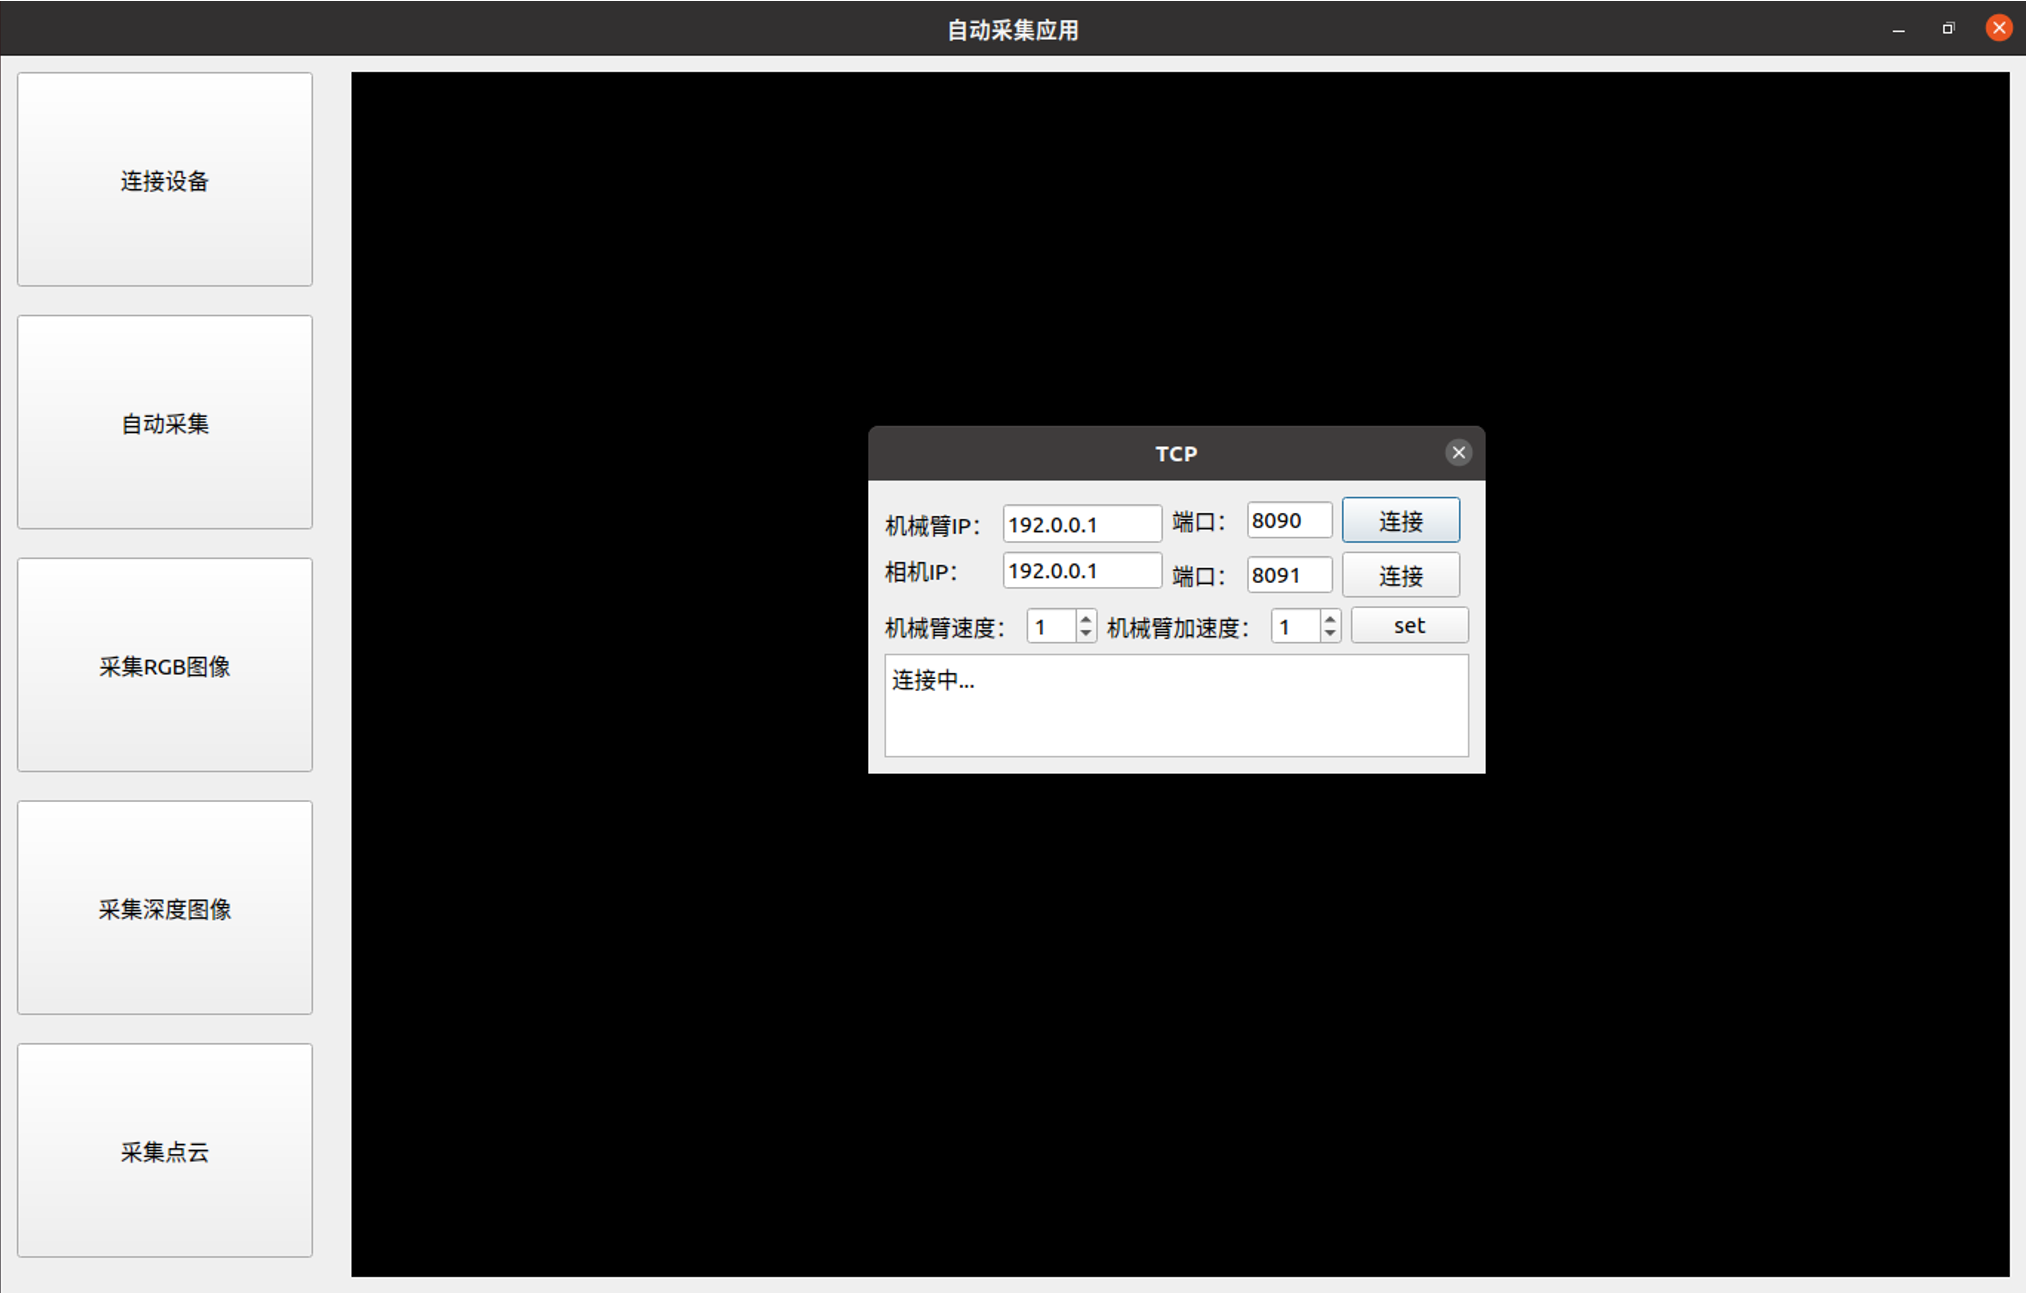
\includegraphics[width=0.75\textwidth]{figures/2/application.png}
  \caption{数据自动采集应用界面}\label{fig:application}
\end{figure}
为了更好地模拟工业实际情况下被检物摆放位置不固定的情况,提高本文缺陷检测实验的效率,本文设计了一个具有可视化交互界面的数据自动采集应用,界面如图\ref{fig:application}所示。这个应用能够一键采集被检对象在指定场景下的数据并打包生成原始数据集,使其可以供后续缺陷检测算法使用。在本文的实验过程中,该应用大大提高了数据采集的效率,并且能够更好地模拟实际工业场景,从而更全面地评估缺陷检测算法的性能。

\begin{figure}[htbp]
  \centering
  \includegraphics[width=0.5\textwidth]{figures/2/capflow.pdf}
  \caption{数据自动采集应用流程图}\label{fig:capflow}
\end{figure}

数据自动采集应用主要由设备连接和数据自动采集两部分构成,流程如图\ref{fig:capflow}所示。其中设备连接部分主要是调用结构光相机和协作机器人提供的SDK中的设备连接API,并使用Qt制作交互界面,供用户输入相机和机器人的IP地址进行握手连接。

数据自动采集部分的核心思路是利用在硬件平台里提到的结构光相机和协作机器人组成的感知硬件系统,通过执行相机采集、回传工控机数据、工控机下达协作机器人关节运动指令、相机再采集的闭环步骤实现多视角数据采集。

其中相机采集步骤,由于梅卡曼德提供的相机SDK中直接输出的是ply格式的无序点云,而本文需要有序点云。因此本文在原SDK的基础上进行了适配开发,重载了导出函数,实现了导出pcd格式有序点云。回传工控机数据步骤主要是对相机采集的数据进行编号并存储至对应文件夹,从而构建包括训练集和测试集的数据集。工控机存储完数据后触发机械臂控制函数,待机械臂运动至目标点后再触发相机采集数据函数。


\section{评价指标}
本文研究目标为图像级缺陷检测,即着眼于算法对正常样本和缺陷样本分类性能。因此本文主要采用ROC
和AUROC作为本文用于评价算法性能的指标。

在测试时,缺陷检测算法的预测结果有表\ref{tab:matrix}所示的四种可能:当测试样本为正常样本,算法预测也为正常样本,即真正例(True Positive,TP);测试样本为正常样本,但算法预测为缺陷样本,即假负例(False Negative,FN);测试样本为缺陷样本,算法预测也为缺陷样本,即真负例(True Negative,TN);测试样本为缺陷样本,但算法预测为正常样本,即假正例(False Positive,FP)。

\begin{table}[htbp]
  \centering
  \caption{缺陷检测混淆矩阵}\label{tab:matrix}
  \begin{tabular}{@{}cccc@{}} \toprule
       &         & \multicolumn{2}{c}{预测值} \\ \cmidrule(r){3-4}
         &        & 正常=1 & 缺陷=0 \\ \midrule
  \multirow{2}{*}{标签值}	& 正常=1 & TP & FN \\
            & 缺陷=0 & FP & TN \\ \bottomrule
   \end{tabular}
  \end{table}

\subsection{ROC曲线}

ROC(The Receiver Operating Characteristic,受试者操作特征曲线)是一种显示分类模型在所有分类阈值下的性能的图表。这条曲线绘制了两个参数:

真正例率TPR (True Positive Rate),即召回率(Recall):
\begin{equation}
  T P R=\frac{T P}{T P+F N}
\end{equation}

假正例率FPR(False Positive Rate)计算公式如下:
\begin{equation}
  F P R=\frac{F P}{F P+T N}
\end{equation}

ROC图表以FPR为横轴,TPR为纵轴,采用不同分类阈值时的(TPR,FPR)作为坐标绘制ROC曲线。


\subsection{AUROC
}


AUROC(Area under the ROC curve,ROC曲线下面积)是用来衡量二分类机器学习算法性能的一种指标。曲线下面积测量的是从 $(0,0)$ 到 $(1,1)$ 之间整个 ROC 曲线以下的整个二维面积。AUC值的范围在$(0,1)$之间,AUC的值越大表明模型分类能力越好。\cite{bradleyUseAreaROC1997} 

\section{本章小结}
本章为后续缺陷检测算法研究搭建了软硬件系统实验平台,首先介绍了本文用于采集数据的的核心硬件设备结构光相机的原理,然后说明了本文搭建实验平台所需的软件环境和硬件设备,并介绍了如何对相机进行标定。此外,为了更好地采集数据,本章还设计了具有交互界面的自动数据采集的应用。在本章最后,介绍了缺陷检测实验所用到的评价指标ROC和AUROC。
\chapter{基于3D点云的缺陷检测}


\section{引言}
金属件的图像采集对打光有严格要求,光源的照射角度以及强度会严重影响检测结果。如一些直射光源会在金属件上产生类似镜面反射的效果,导致采集的二维图像出现“死白”——即一片像素点为无变化特征的白色像素。3D激光相机往往采用蓝光,其能较好降低金属件的反射对成像的影响,有利于特征的提取,为下游缺陷检测提供输入。

在2D缺陷检测领域,PatchCore作为无监督的方法表现出优异的性能。本文基于点云数据的缺陷检测算法受Horwitz等人\cite{horwitzBackFeatureClassical2022}启发,以PatchCore的特征存储为骨干网络,将二维的Patch迁移到三维的Pillar\cite{langPointPillarsFastEncoders2019a},并通过RoPS三维局部特征描述子来提取点云Pillar的特征并进行存储用于检测缺陷。本文称改进的无监督点云缺陷检测方法为PillarCore,算法的整体框架如图\ref{fig:PillarCore}所示。
\begin{figure}[htbp]
    \centering
    \includegraphics[width=1\textwidth]{figures/3/3-framework.pdf}
    \caption{PillarCore框架}\label{fig:PillarCore}
\end{figure}

本章首先将介绍如何组合多种点云滤波方法对输入点云进行预处理,其次将介绍如何通过贪婪投影将点云三角化,接着介绍本文引入的RoPS特征描述子的原理,然后介绍本文基于的PatchCore方法是如何工作的,最后本文展开了多项实验并充分验证说明本文提出的PillarCore算法在无监督点云缺陷检测上的性能表现。



\section{点云预处理}
\subsection{点云直通滤波}

% \begin{figure}[htbp]
%     \centering
%     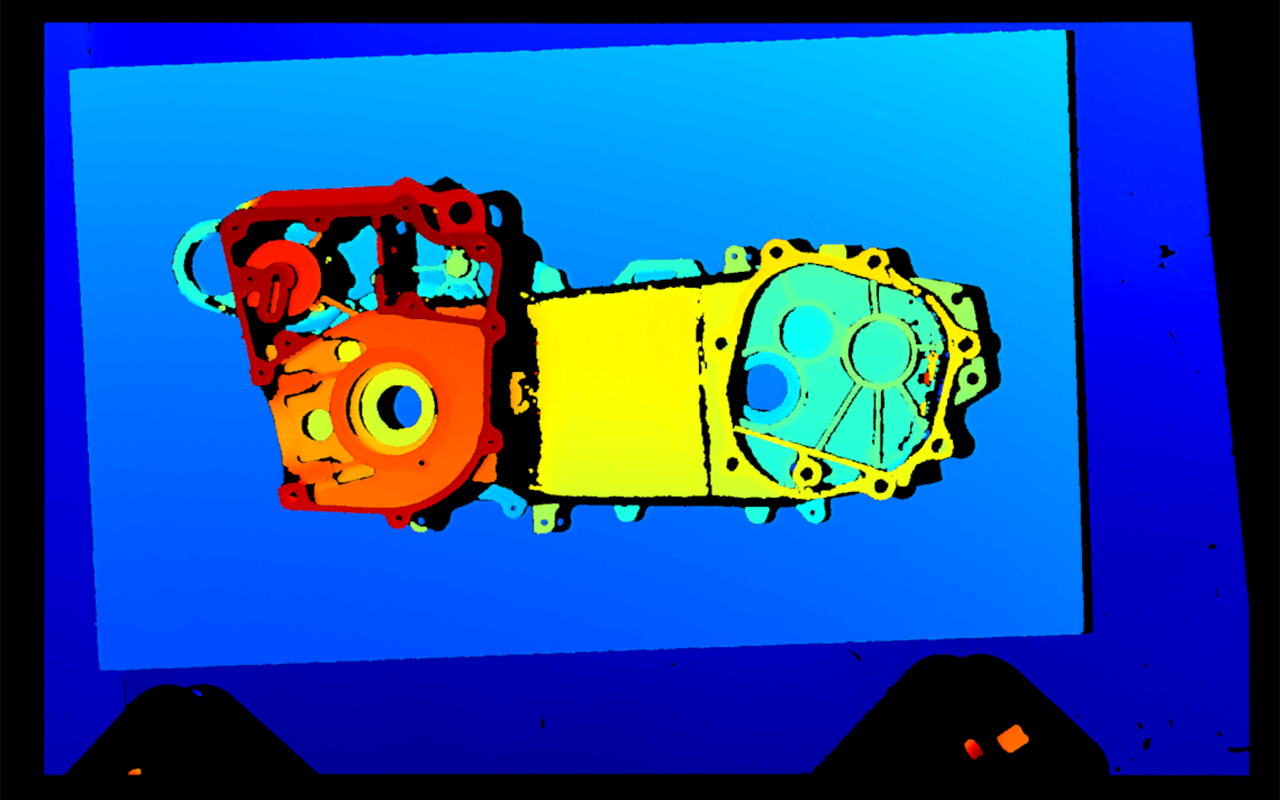
\includegraphics[width=0.75\textwidth]{figures/xy_before_passthrough.png}
%     % \caption[这里的文字将会显示在 listoffigure 中]{这里的文字将会显示在正文中}
%     \caption{原始点云俯视图}\label{fig:xy_before_passthrough}
% \end{figure}

\begin{figure}[htbp]
    \centering
    \begin{subfigure}
        \centering
        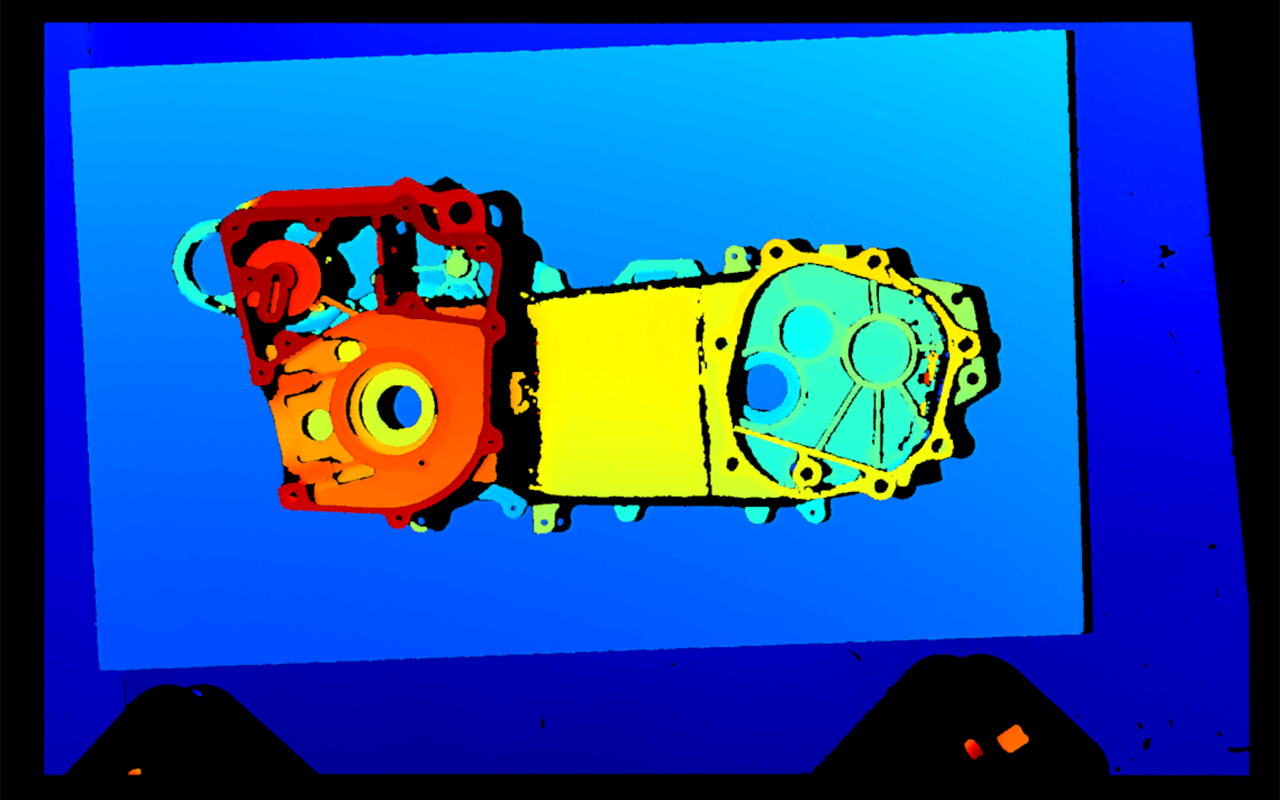
\includegraphics[width=.45\linewidth]{figures/xy_before_passthrough.png}  
      \end{subfigure}
      \begin{subfigure}
        \centering
        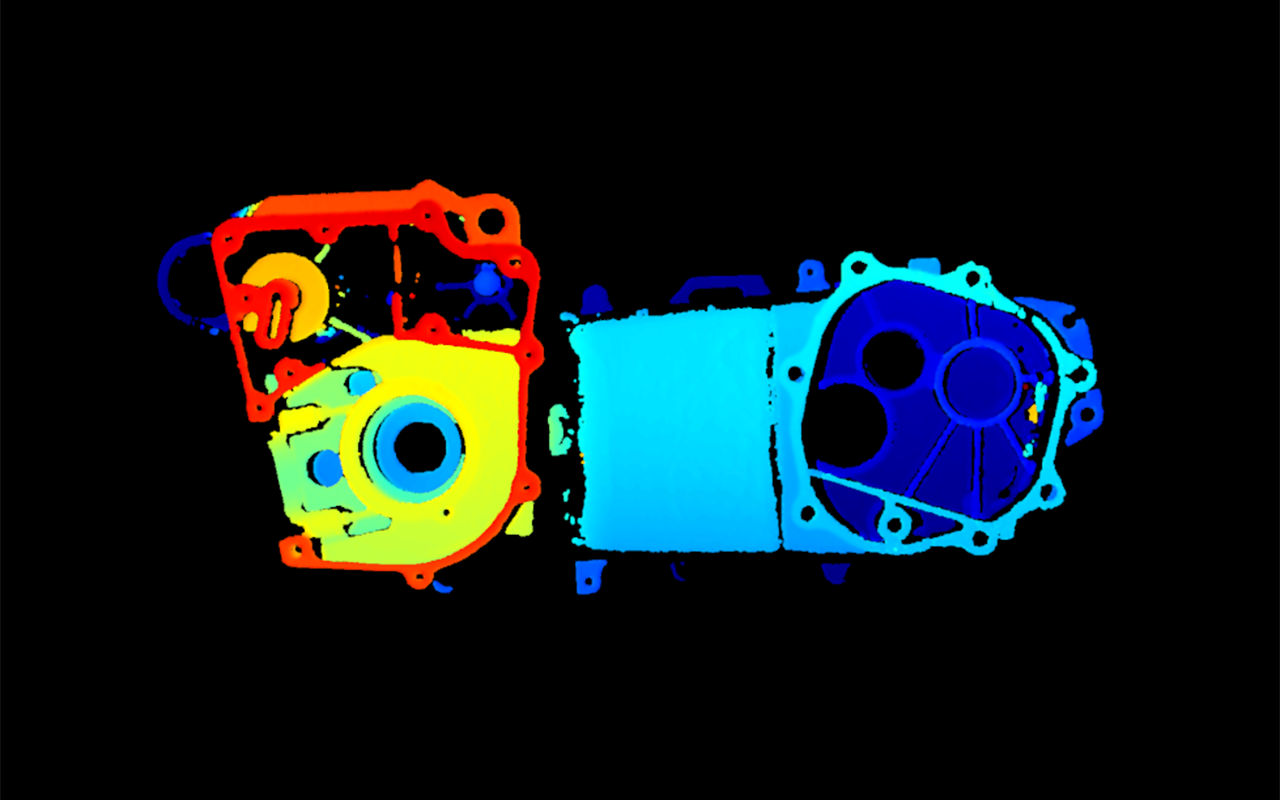
\includegraphics[width=.45\linewidth]{figures/z_xy_afterpassthrough.png} 
      \end{subfigure}
    \caption{直通滤波前后效果}
    \label{fig:xy}
\end{figure}

本文为覆盖多种目标,使用的相机FOV较大,因此会有较多与目标缺陷检测无关的背景被同时采集,如图\ref{fig:xy}中左图所示。直通滤波是一种高效易用的点云滤波方法,其原理是将所有点在指定维度上(如x,y,z轴)与设定的最小值和最大值进行比较,只有在范围内或范围外的点才被保留,其它点则被过滤掉。

直通滤波主要有两大作用。一是通过对点云数据进行直通滤波,能快速去除偏差较大的离群点,降低噪声对后续缺陷检测任务计算结果的影响;二是在点云处理中,直通滤波可以根据设定的范围提取出感兴趣区域的点云,从而实现缩小点云规模,减少后续任务计算量,提高计算效率。
\begin{figure}[htbp]
    \centering
    \begin{subfigure}
        \centering
        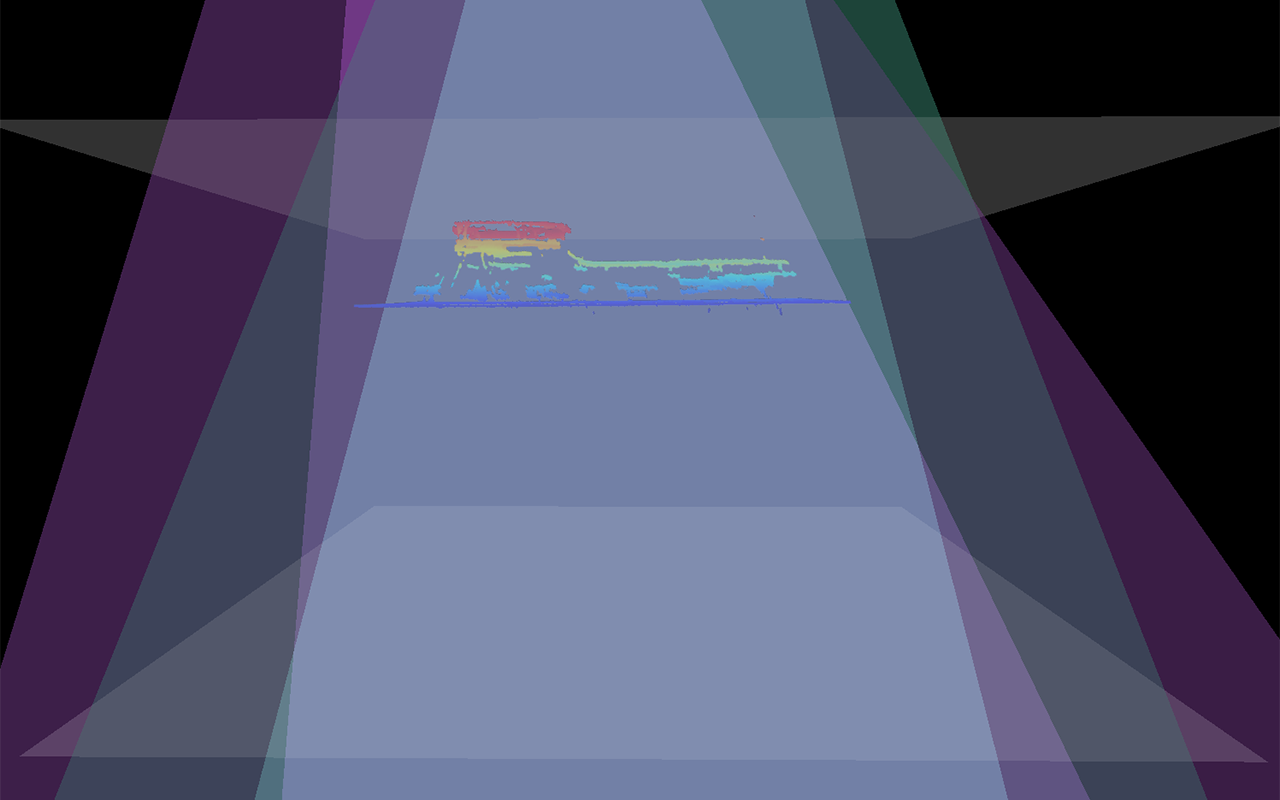
\includegraphics[width=.45\linewidth]{figures/z_before_passthrough.png}  
      \end{subfigure}
      \begin{subfigure}
        \centering
        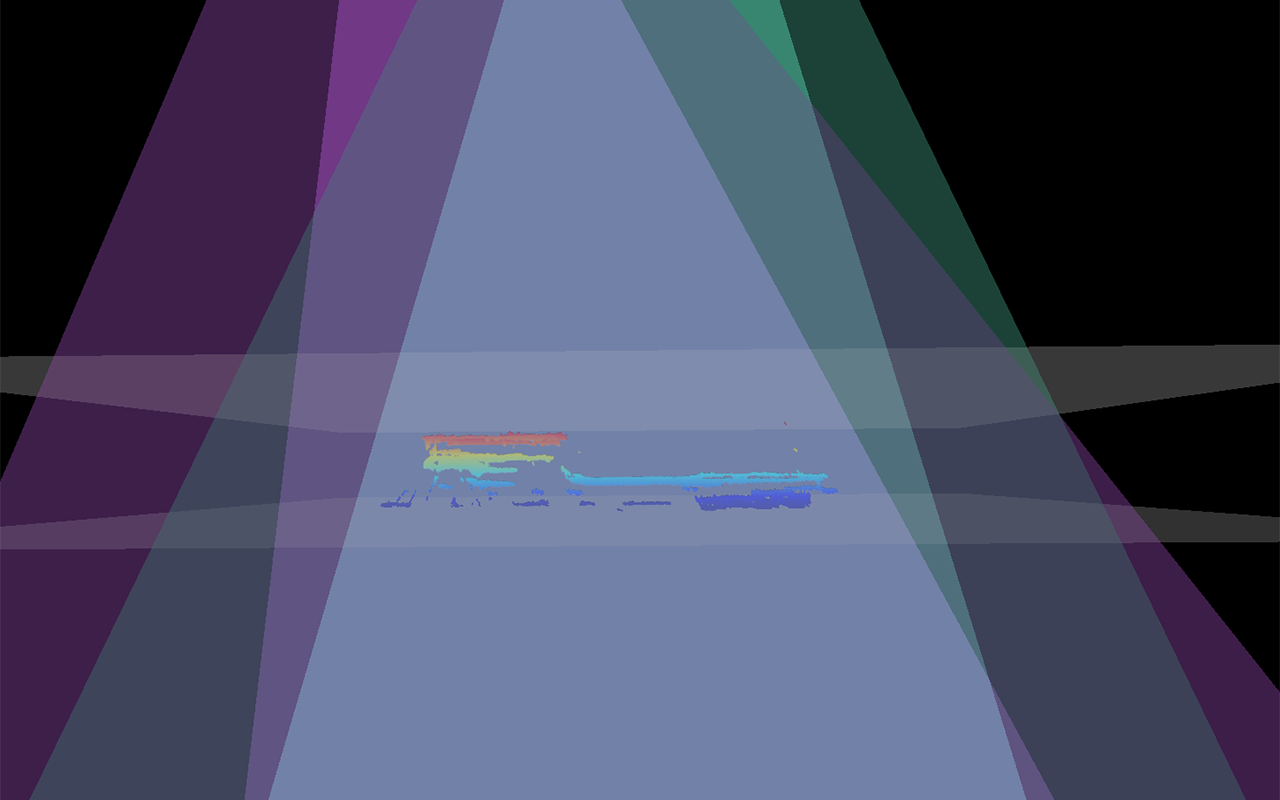
\includegraphics[width=.45\linewidth]{figures/z_after_passthrough.png} 
      \end{subfigure}
    \caption{z轴直通滤波示意图}
    \label{fig:z}
\end{figure}

因此,直通滤波方法常见于各种点云算法的预处理阶段,用来提升算法输入点云的质量。本文研究的对象近似为空间中的立方体,通过分别沿x,y和z轴对点云数据进行直通滤波的预处理,可以实现提取后续缺陷检测任务的ROI区域。其中Z轴直通滤波示意如图\ref{fig:z}所示。

% \begin{figure}[htbp]
%     \centering
%     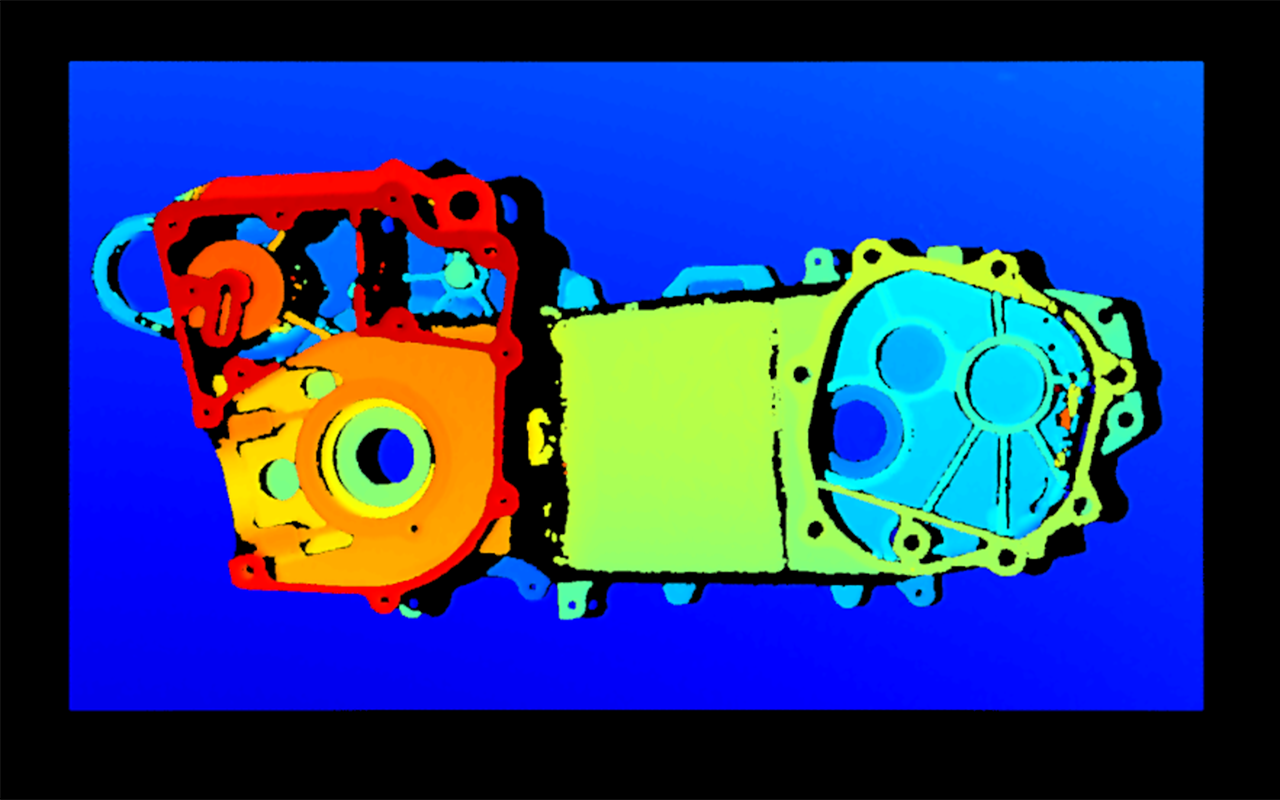
\includegraphics[width=0.75\textwidth]{figures/xy_after_passthrough.png}
%     \caption{按x、y轴对点云直通滤波后俯视图}\label{fig:xy_after_passthrough}
% \end{figure}



% \begin{figure}[htbp]
%     \centering
%     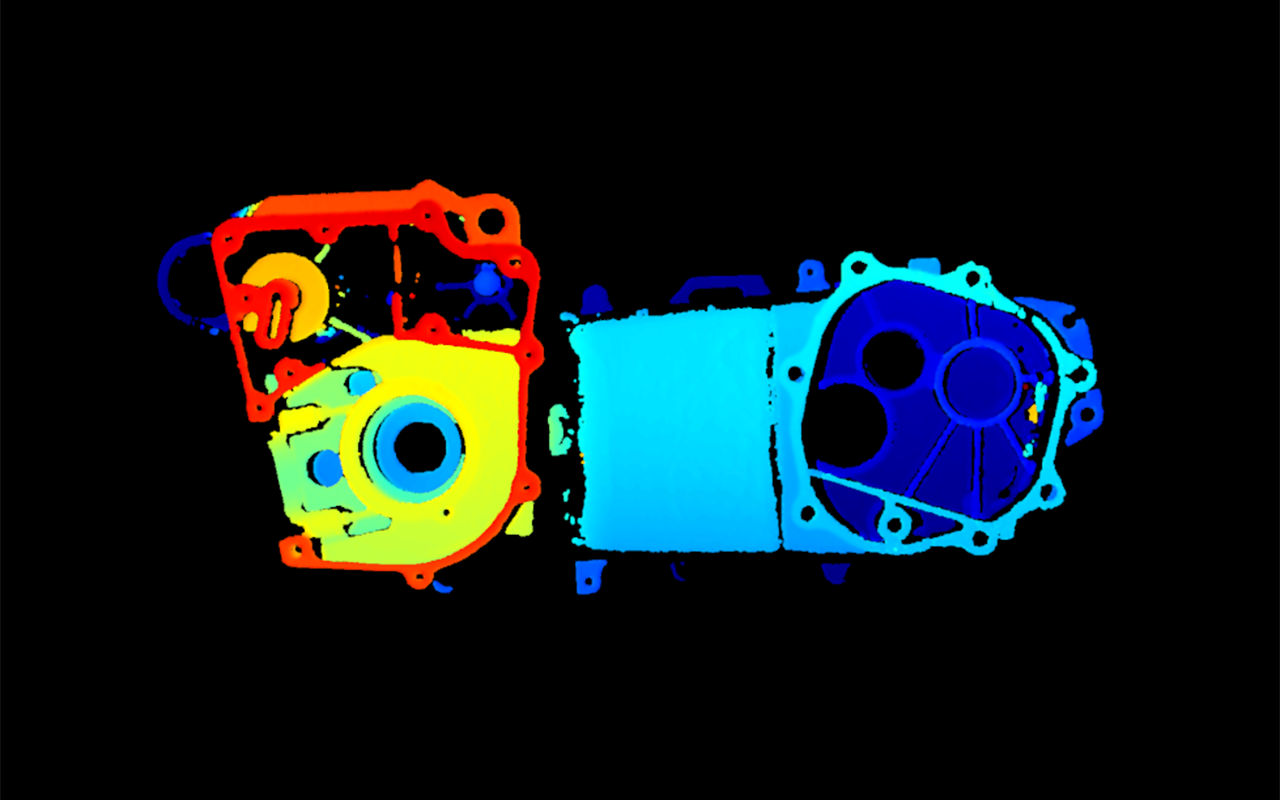
\includegraphics[width=0.75\textwidth]{figures/z_xy_afterpassthrough.png}
%     \caption{按z轴对点云直通滤波后俯视图}\label{fig:z_xy_afterpassthrough}
% \end{figure}



\subsection{点云统计滤波}
离群点是指与其余数据显著不同的点,通常是测量误差或其他异常的结果。本文使用的光栅结构光相机,在采集过程中,面对反光严重的金属件,相机输出的点云数据中存在不少肉眼可观察的离群点,可以预见会对后续缺陷检测任务的准确性和效率产生较大影响。

点云统计滤波是一种用于减少点云数据中噪声的技术,其原理是通过分析数据的统计属性并剔除被判定为离群点的点来实现。点云数据有几种可用的统计滤波器,包括均值、中位数、标准偏差和方差滤波器。这些滤波器都基于数据的统计属性进行操作。

点云统计滤波包括三个主要步骤:数据预处理、统计分析和数据滤波。首先是对点云数据进行预处理,即将原始点云数据转换为可以由统计滤波算法处理的矩阵或数组格式。当数据经过预处理后,接着就可以进行统计分析。常见的统计属性包括均值、中位数、标准偏差和方差等,这些统计属性然后被用来识别离群点。

最后一步是通过删除已识别的离群点来过滤数据。所使用的具体滤波算法将取决于数据的统计属性和应用程序。统计滤波输出的结果是一个已经清理噪声且更适合进一步处理的点云数据集,其效果如图\ref{fig:statistic}所示,其中红色标记的点是统计滤波滤出的离群噪声点。
\begin{figure}[htbp]
    \centering
    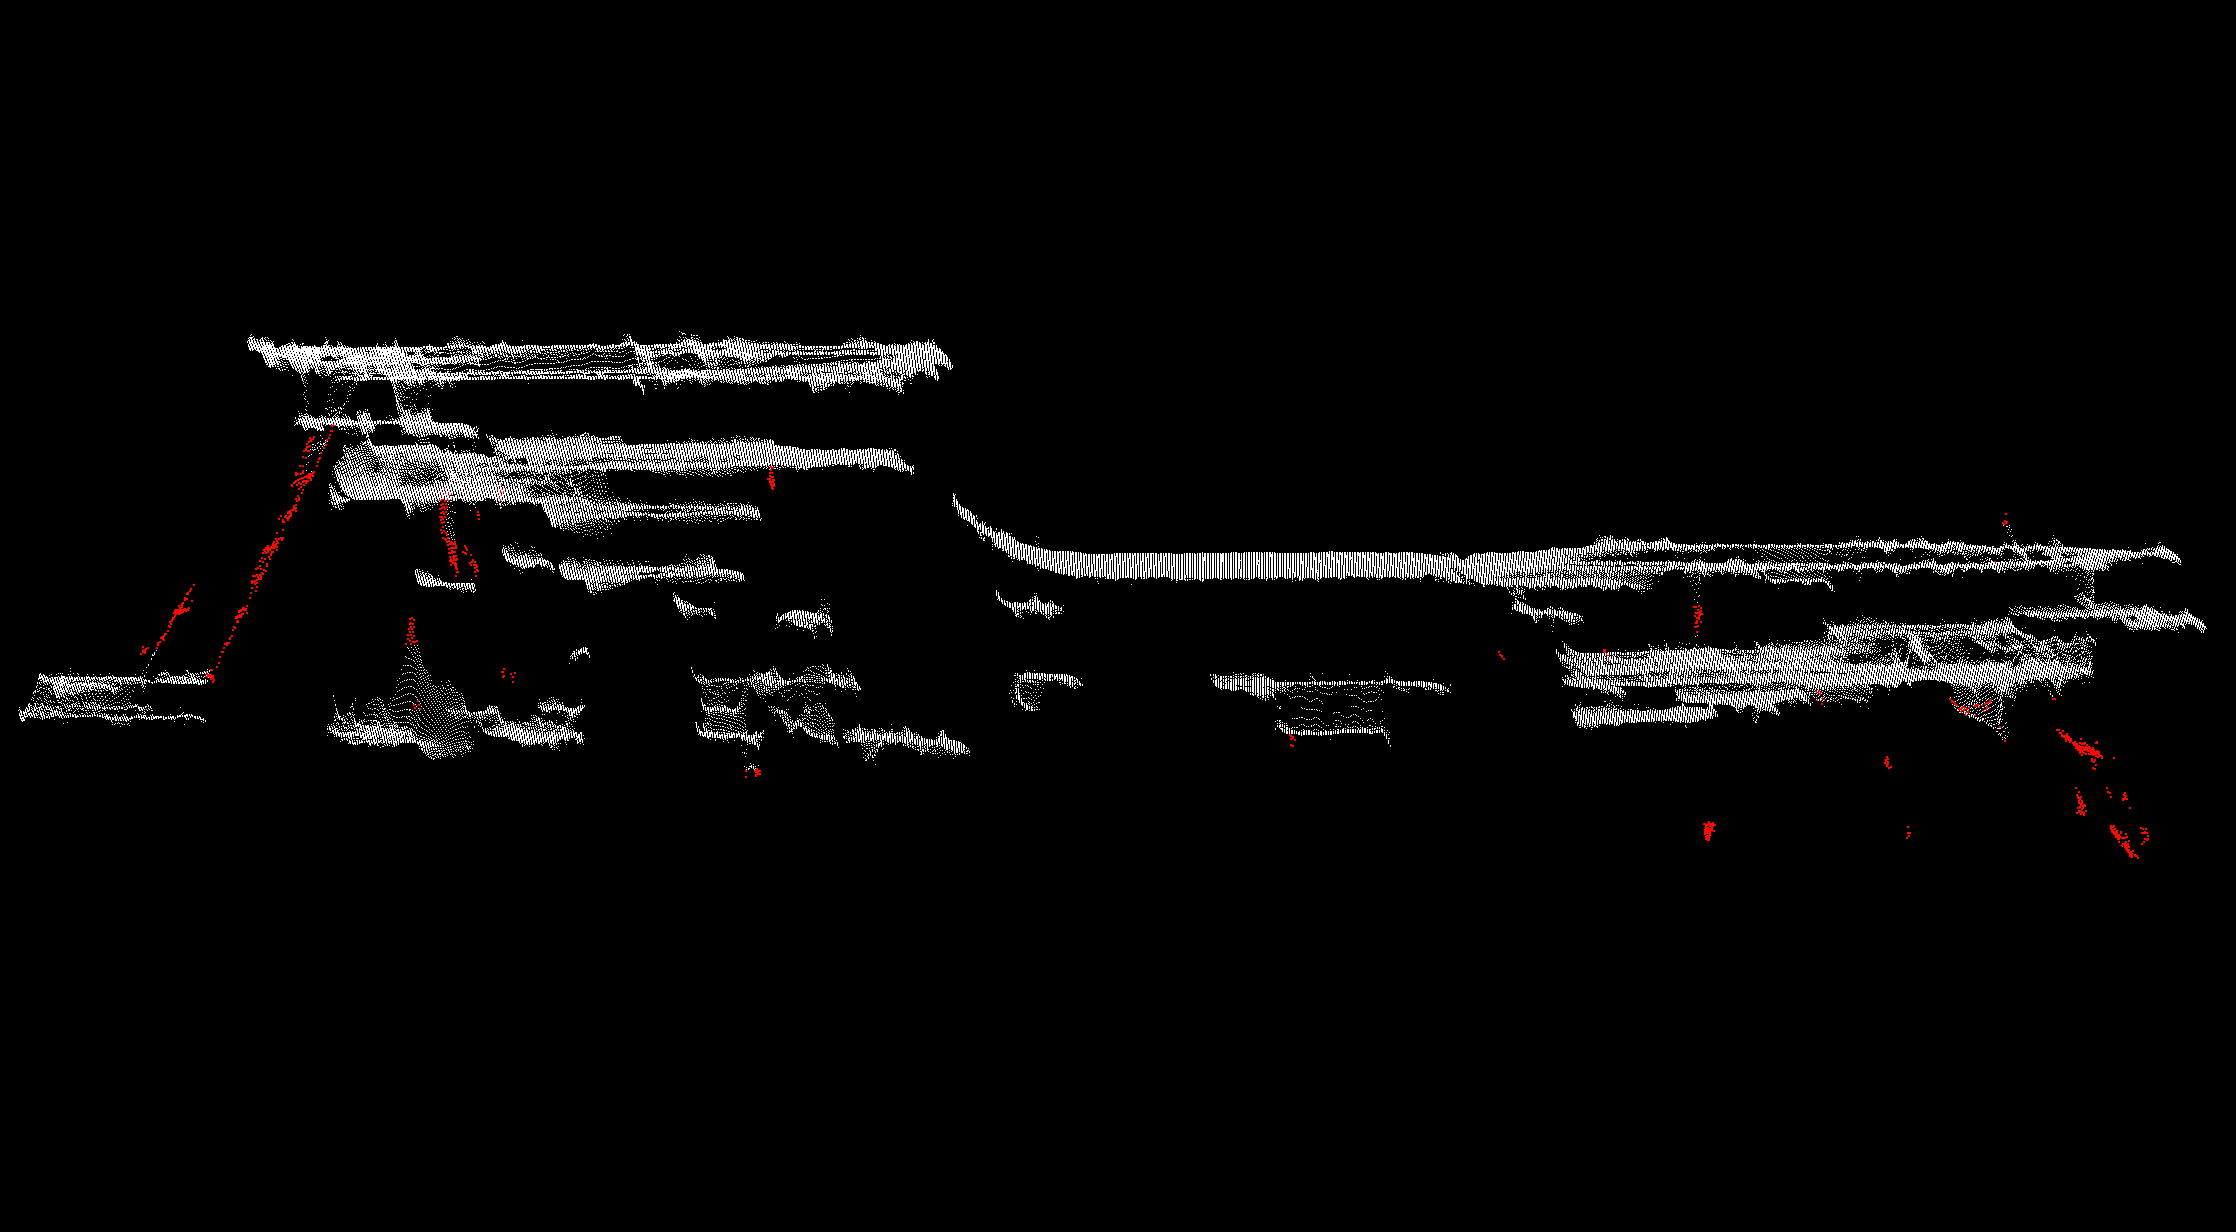
\includegraphics[width=0.75\textwidth]{figures/statistic.png}
    \caption{统计滤波侧视图}
    \label{fig:statistic}
\end{figure}

值得一提的是,对于一些结构简单,特征明显的物体,例如正常样本为平整表面的被检物,统计滤波算法可以直接用于对其进行缺陷检测。由于本文聚焦的是更为复杂的非平整表面,无法直接通过统计滤波实现理想的缺陷检测,但通过统计滤波能有效减少噪点,提升后续缺陷检测任务的准确性和效率,因此统计滤波只作为本文缺陷检测任务中点云预处理的一部分。


\subsection{点云下采样}
通常来说,结构光相机采集的点云数据非常庞大,以本文使用的梅卡曼德相机来说,其分辨率为$1920 \times1200$ ,每个点云数据点数约有两百万个点,单个点云存储文件约二十兆。即使经过前述直通滤波和统计滤波,提取出的ROI低噪声点云仍然有约三十万个点。稠密的原始点云能有效表现被摄物细节,但随之而来的是后续任务巨大的计算量。特别在工业生产环境下,时间就是金钱,企业不仅追求缺陷检测的算法性能,还同样关注算法的效率。

实际上在这些原始稠密点云中,有些点对于特征表现的贡献很小却依然会被计算。因此需要通过点云下采样在保留原始点云重要几何特征的同时减少点云中的点数,从而缩小点云整体规模,提升后续算法的计算效率。

点云下采样有不同的方法,例如随机,均匀或基于网格。本文采用基于网格的体素滤波进行下采样。体素滤波是一种对点云进行下采样的方法,它把三维空间划分成多个小立方体,然后用每个立方体的中心点或质心来近似该立方体内的所有点。
\begin{figure}[htbp]
    \centering
    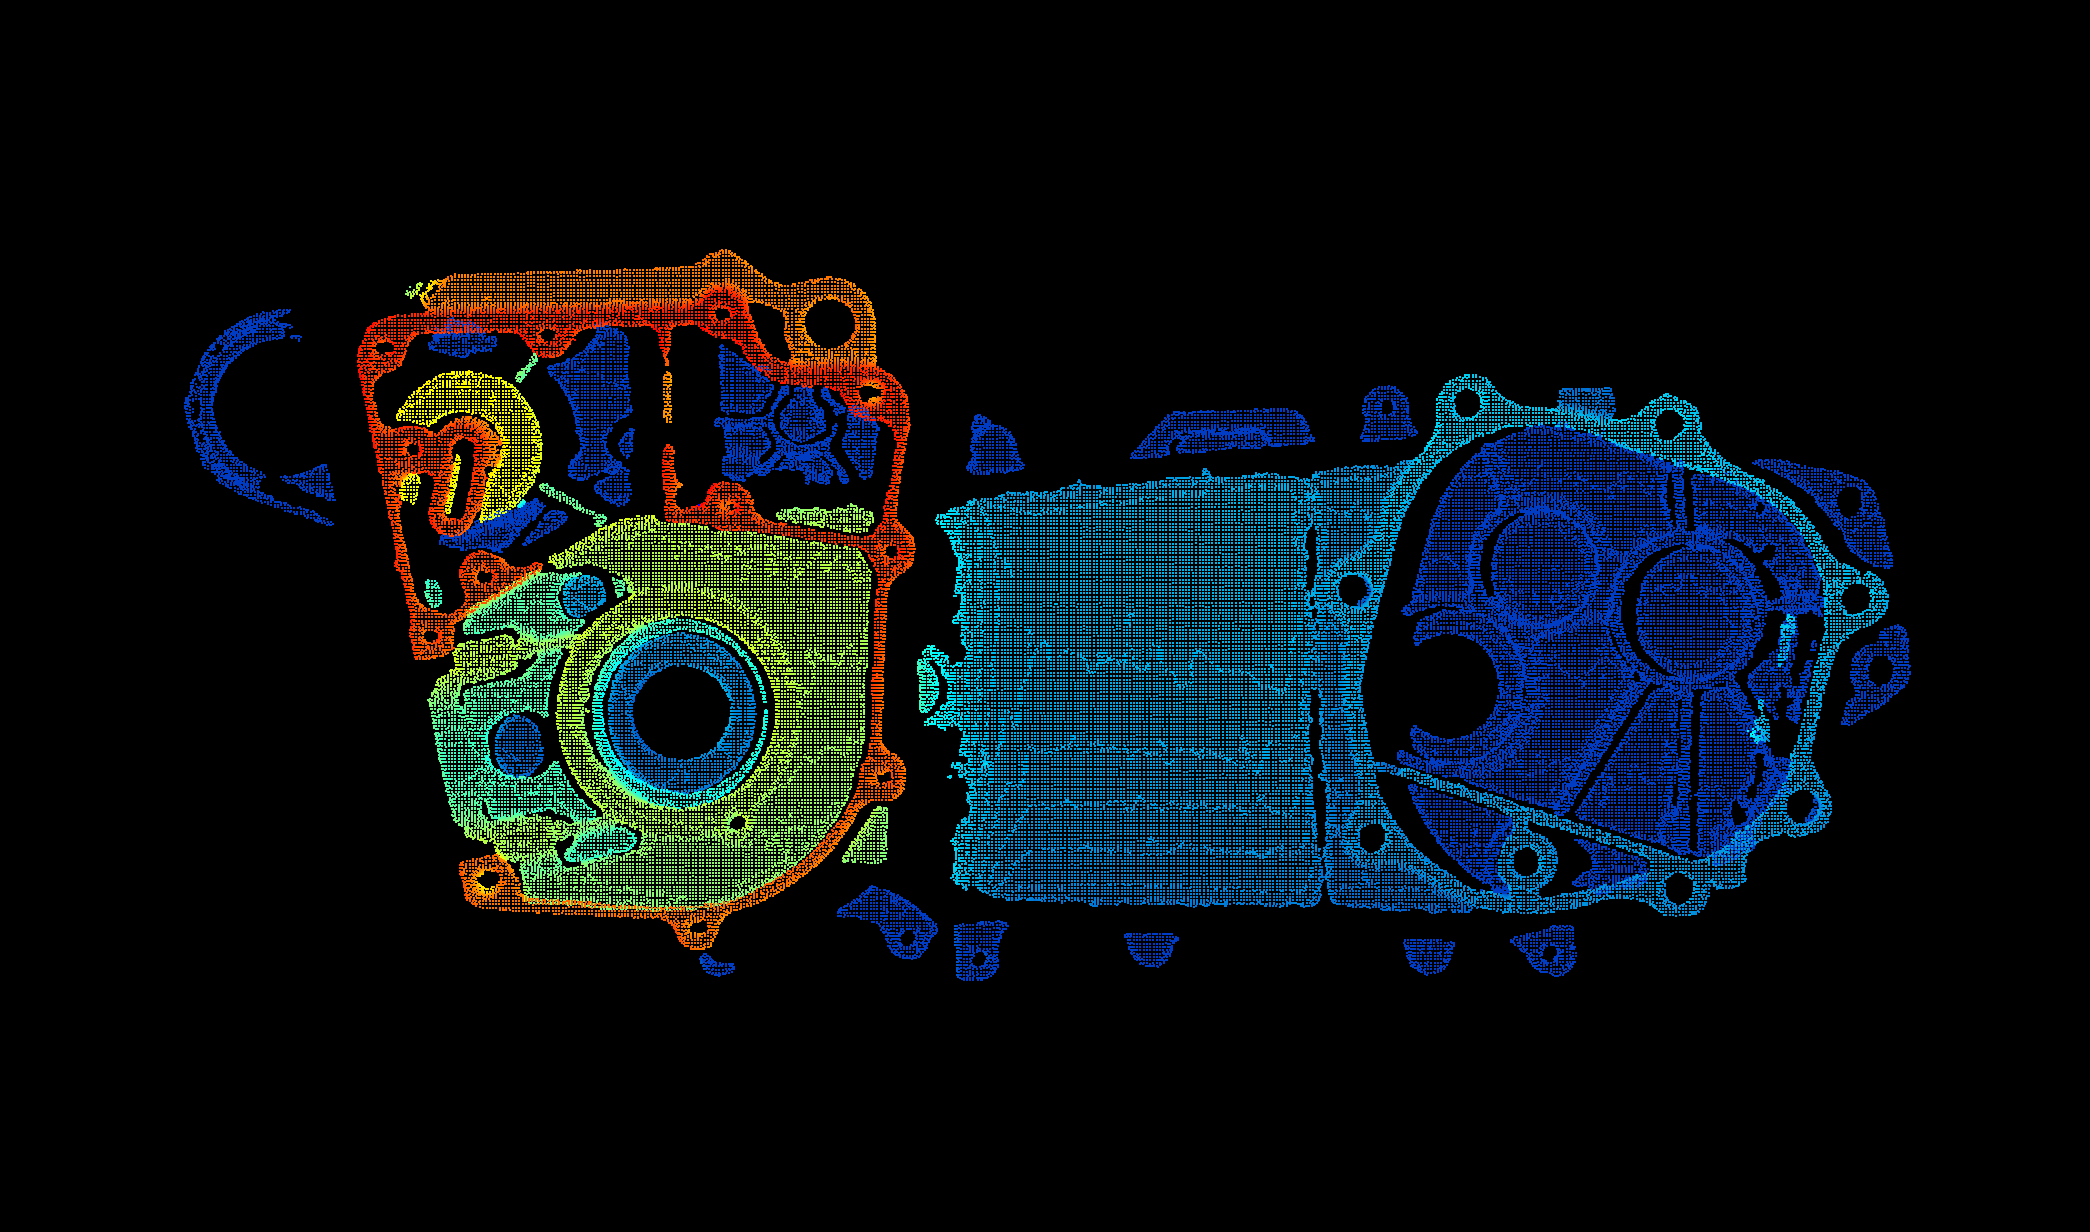
\includegraphics[width=0.75\textwidth]{figures/after_down.png}
    \caption{点云体素滤波效果图}
    \label{fig:aftet_down}
\end{figure}

网格大小是体素滤波的一个重要参数,网格太大,可能会导致原始点云的形状和特征丢失,甚至出现空洞和失真;网格太小,可能会导致下采样效果不明显。选择合适的网格大小才能既减少点云数据量,又保持原始点云的集合结构。本文经过多次实验选择0.001作为网格大小进行体素滤波,以采集的一个正常样本为例,体素滤波效果如图\ref{fig:aftet_down}所示。



\section{点云网格化}
\subsection{点云法线估计}
表面法线是在给定点垂直于表面的矢量。法向量表示表面的方向,可以用来提取对物体旋转和平移不变的特征。在点云和网格的情况下,可以通过计算每个点周围的局部几何来估计法向量。

估计一个点的法向量的最简单方法是使用最适合一小组相邻点的平面的表面法线。这被称为 PCA(主成分分析)方法,它涉及计算局部点云的协方差矩阵的特征向量。具有最小特征值的特征向量对应于局部表面的法向量。法线估计的效果如图\ref{fig:normal_estimation}所示,其中黑色箭头为估计的法向量。
\begin{figure}[htbp]
    \centering
    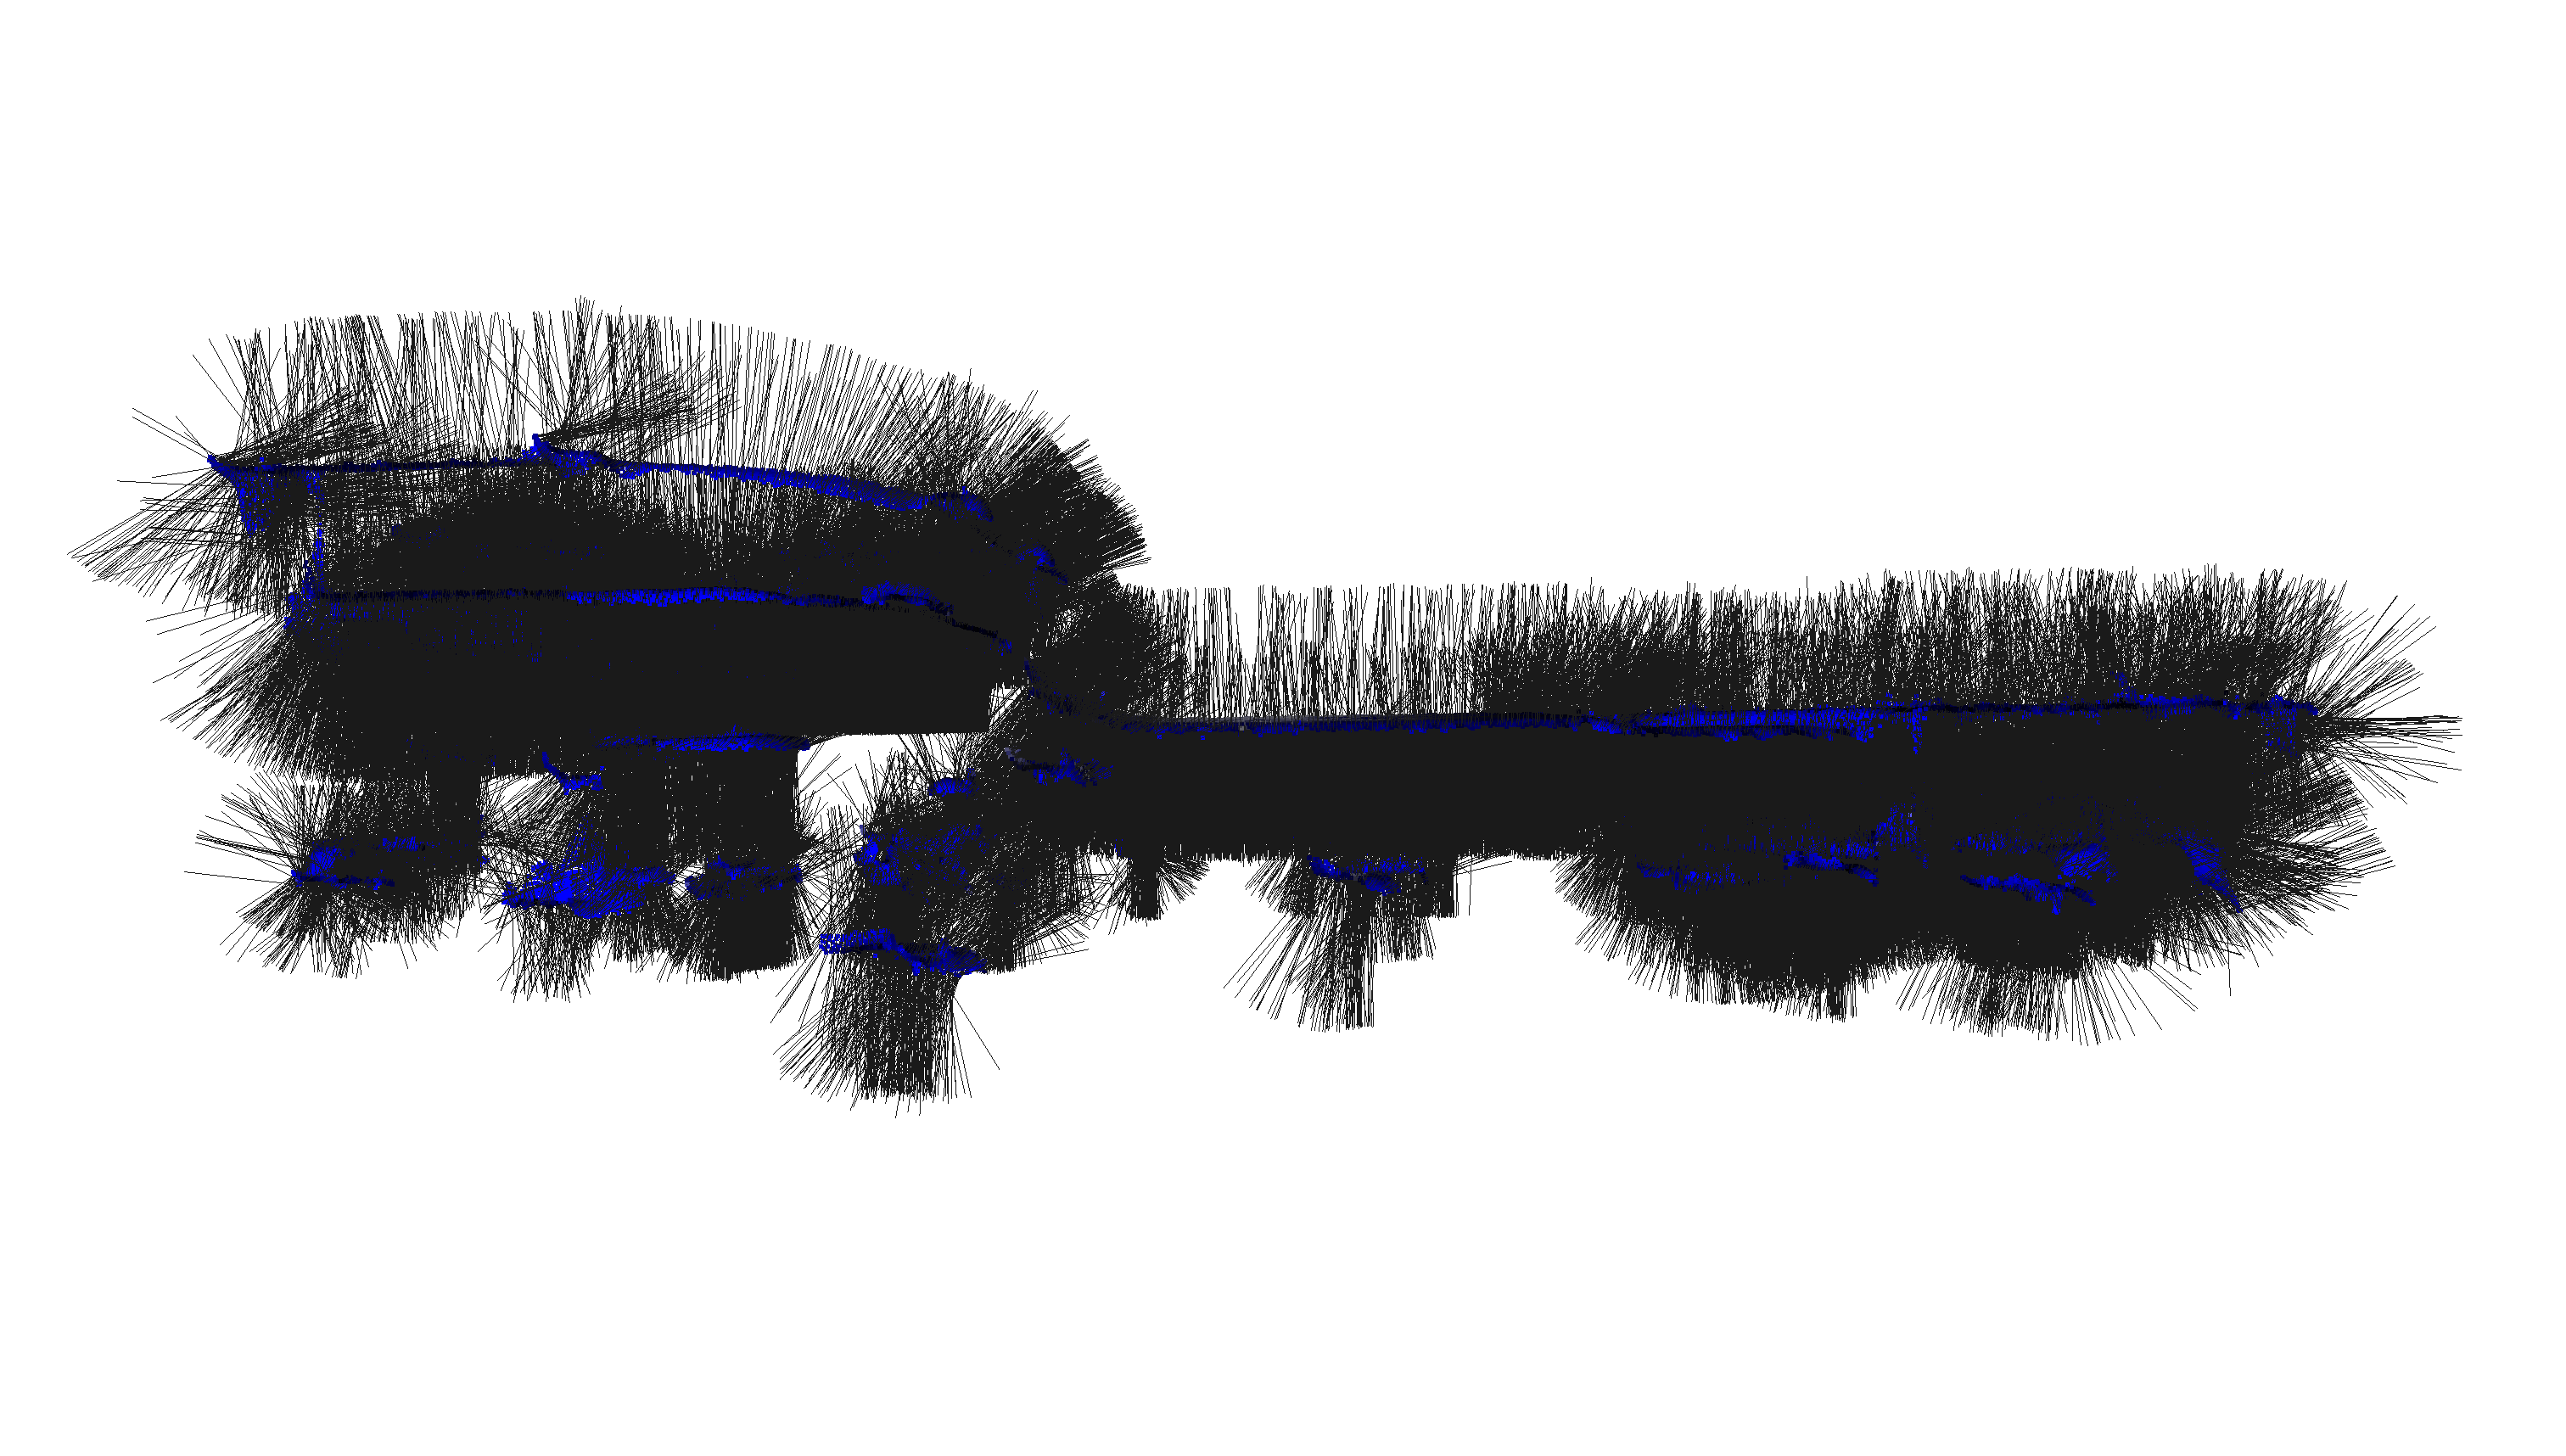
\includegraphics[width=0.75\textwidth]{figures/normal_estimation.png}
    \caption{法线估计侧视图}
    \label{fig:normal_estimation}
\end{figure}

\subsection{贪婪投影三角化}
Gopi等人\cite{gopiFastEfficientProjectionbased2002}使用贪婪投影三角网格化点云,其原理是维护一个点的列表,然后通过列表中的点不断延伸(即加入新的点)来构建网格,直到连接所有可能的点。其中三角剖分是面向局部的,先沿法线方向投影点的局部邻点,然后连接尚未连接的点以构建网格。
该算法基于增量表面生长原理,遵循贪婪方法。该算法从创建一个起始三角形开始,并不断添加新的三角形,直到覆盖所有点云中的点,或者没有更多可以加入到网格中的有效三角形。贪婪投影三角化的具体步骤如下:

第一步进行最近邻搜索,对于点云中的每个点 $p$,选择其k近邻。这个邻域通过搜索以参考点为球心、半径为$r$的球体中的最近k个邻点来定义。半径定为 $\mu .d$,其中$d$是点$p$到其最近邻点的距离,$\mu$是根据点云密度自定义的常数。通常使用Kdtree最近邻算法来寻找给定点的最近邻。

第二步进行切平面邻域投影,将邻域沿参考点$p$的法向量投影到与邻域形成的曲面近似相切的切平面上,并按角度排序。

第三步进行剪枝,按可视性和距离标准对邻域点进行剪枝,依次连接邻域点到参考点$p$和连续点,形成有最大角度约束和可选最小角度约束的三角形。其中遵循距离标准剪枝可以减少用Kdtree对当前点空间近似区域内候选邻接点的搜索。

\begin{table}[htbp]
    \centering
    \caption{贪婪投影三角化中点的类型} \label{tab:point-triangle}
    \begin{tabular*}{0.75\textwidth}{@{\extracolsep{\fill}}cc}
    \toprule
      类型&定义\\
      \midrule
      自由点&没有邻接三角形\\
      完成点	&所有邻接三角形都已确定\\
      边界点	&最大允许角度约束而缺失三角形的参考点\\
      边缘点	&尚未被选择作为参考点\\
    \bottomrule
    \end{tabular*}
\end{table}

可视性是用来排除可能产生自交网格的点。根据点在贪婪投影三角化算法中的状态,可以将其分为如表\ref{tab:point-triangle}所示的四种类型,在初始化时,点云中的点都是自由点。算法定义了两种边缘类型来检查可视性,一种是连接边缘点或边界点,只参与形成一个三角形边的边界边;另一种是连接完成点和其他点的内部边。使用参考点、候选点集以及边界边投影平面,如果从参考点到候选顶点的视线被边遮挡,则该点将被遮挡。

第四步是选择投影平面。将通过距离标准筛选的候选点集投影到近似切平面上,其中候选点为参考点为球心、半径为$r$球体内的所选点。

第五步是按角度排序。一个新的局部坐标系以参考点为坐标原点,以投影的平面为xy平面,所有候选点集中的点都被投影到该平面。候选点的角度是指局部坐标系x轴和从原点到投影后的候选点的向量间的夹角,并基于该角度进行排序。

按照上述步骤对点云进行贪婪投影三角化的效果如图\ref{fig:triangle}所示。

\begin{figure}[htbp]
    \centering
    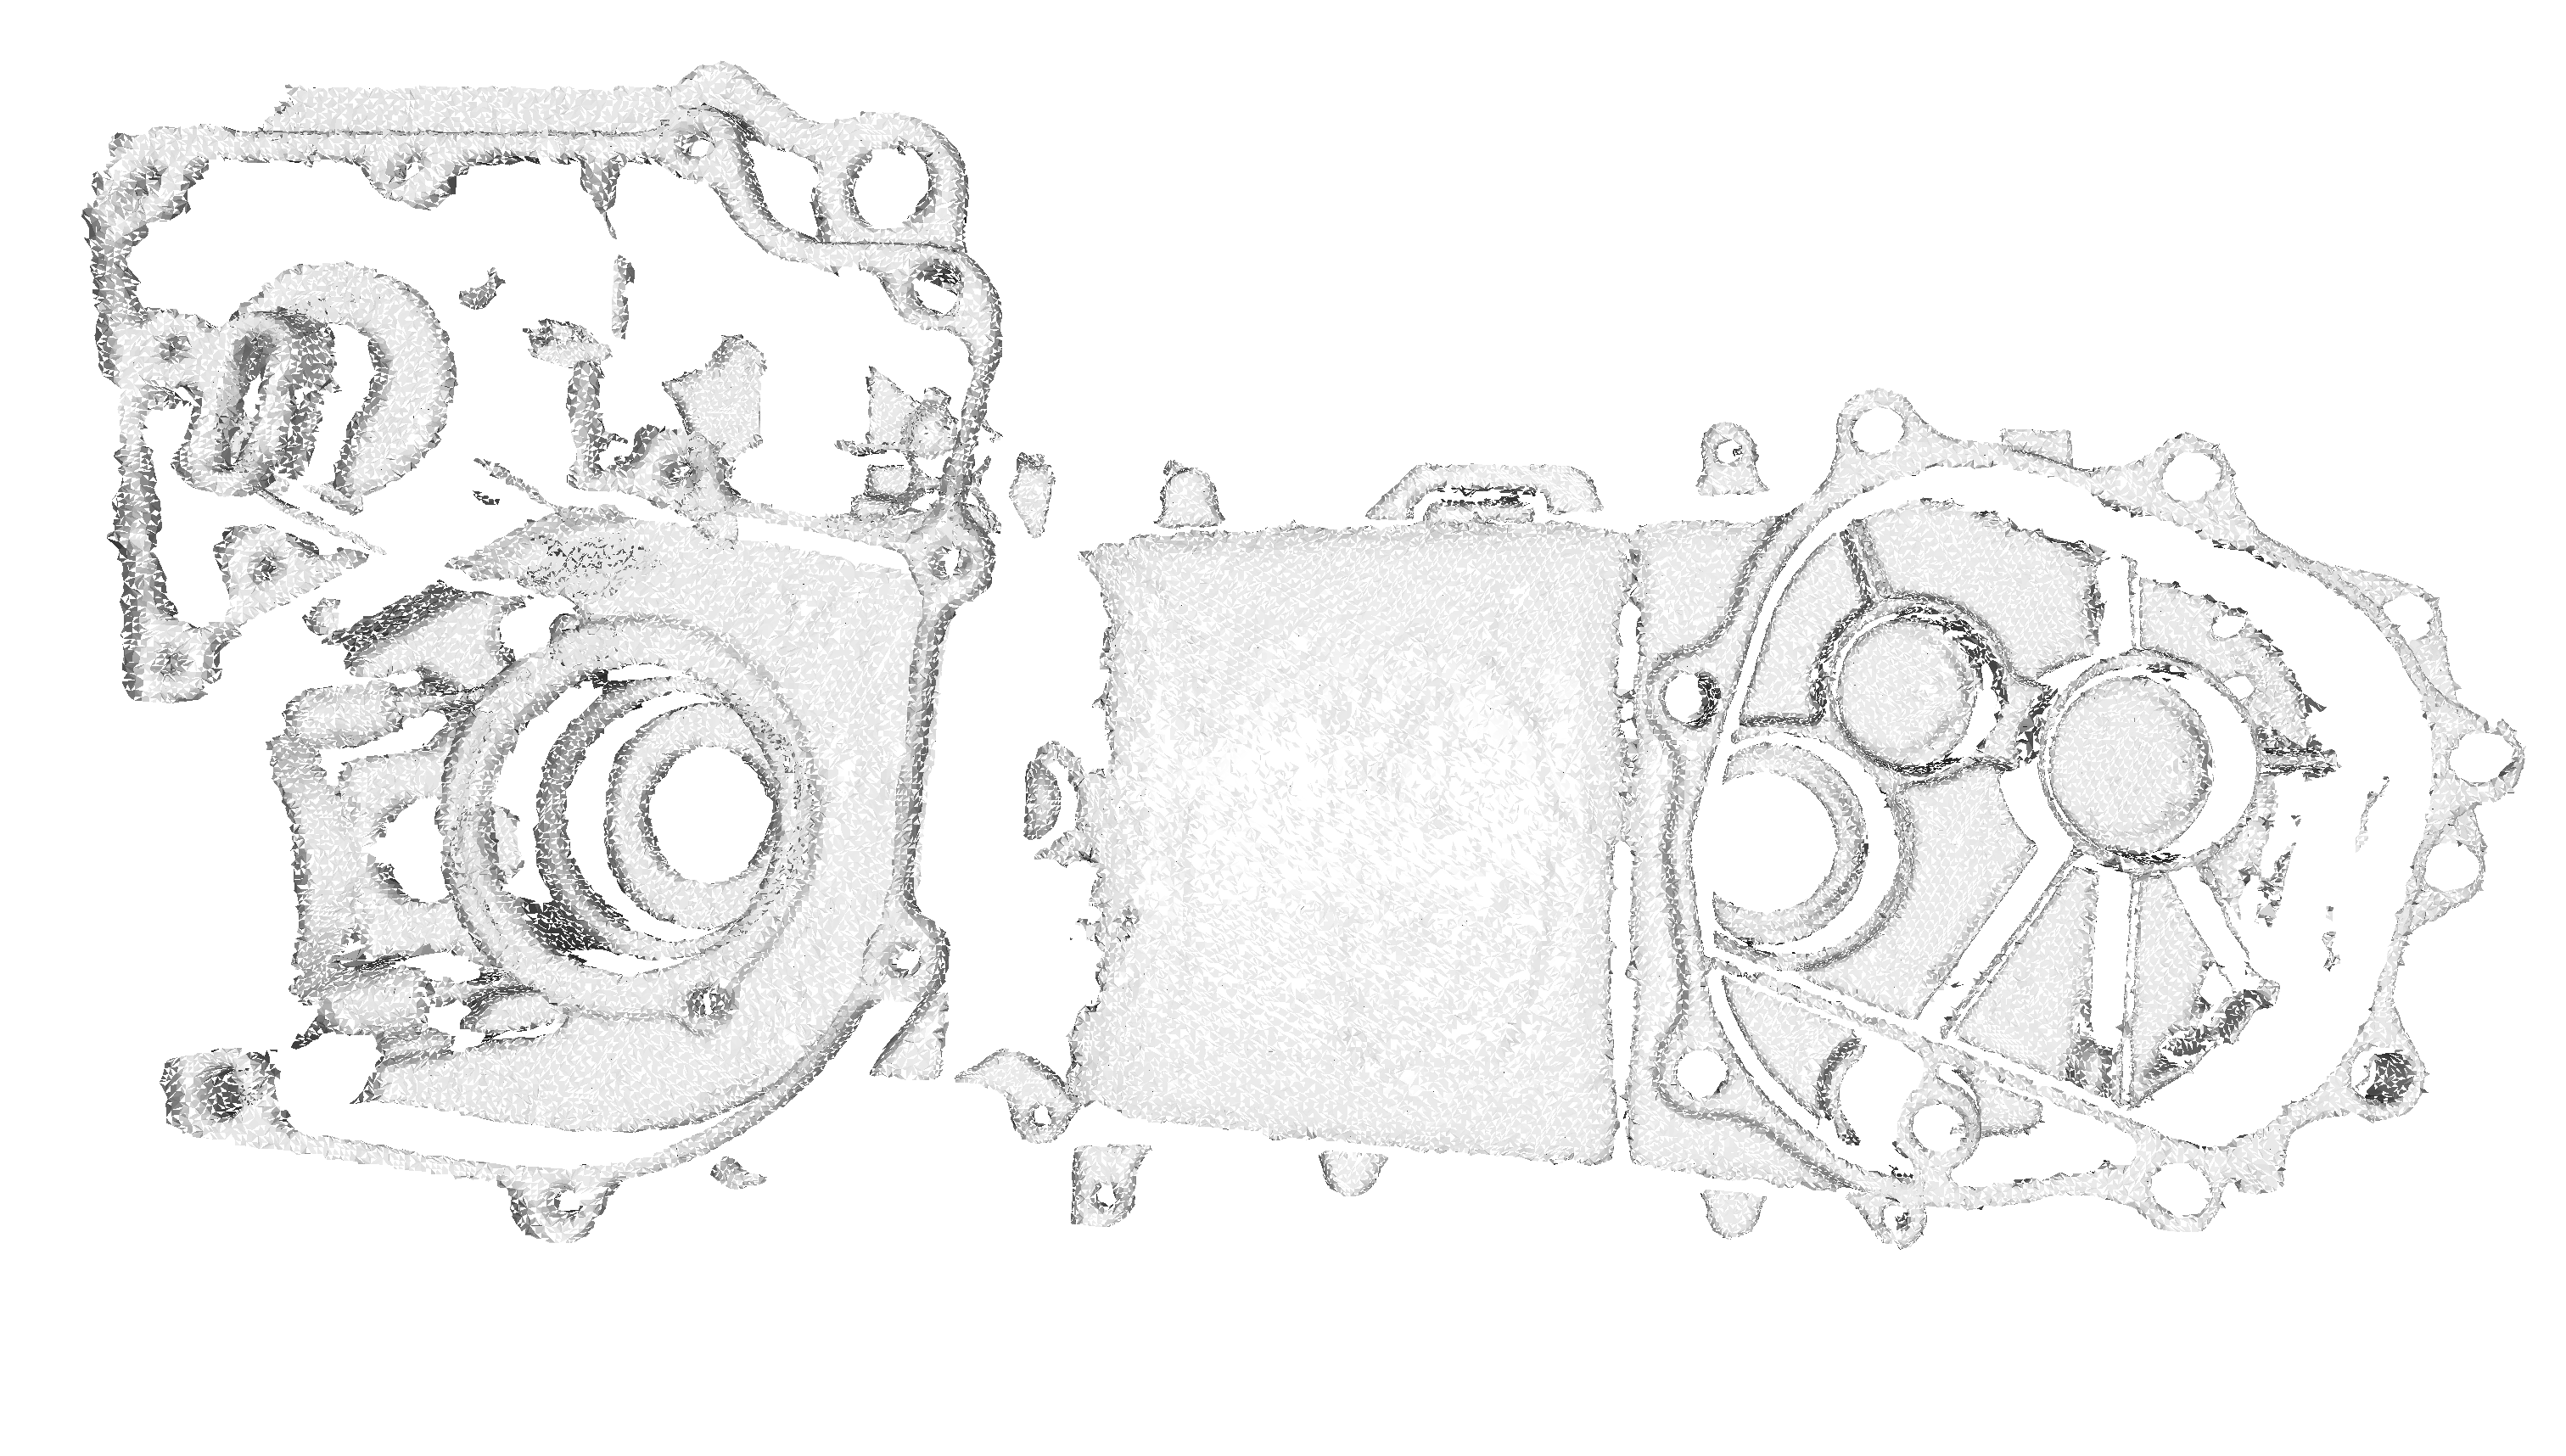
\includegraphics[width=0.75\textwidth]{figures/triangle.png}
    \caption{点云三角网格化}
    \label{fig:triangle}
\end{figure}

\section{点云局部特征提取}
RoPS\cite{yulanguoRoPSLocalFeature2013}是基于空间分布直方图的描述子,其构建的LRF(local reference frame)是独特且可重复的。RoPS算法包含两个部分。 首先,为每个关键点构造一个 LRF,并将局部表面与 LRF 对齐,以实现对刚性变换的不变性。 然后局部表面上的点分别绕三个坐标轴(即 x、y 和 z)旋转。 对于每次旋转,支撑区域中的点进一步投影到三个坐标平面(即 xy、yz 和 xz)上。

通过将平面划分为几个区间(bin)并计算落入每个区间的点数,为每个平面生成一个分布矩阵。 随后用五个统计量对分布矩阵进行编码。最后,通过连接所有旋转和投影的所有这些统计数据生成 RoPS 描述子。 RoPS 描述符的维度是$3\times3\times5\times drops_{r}$,其中 $drops_{r}$ 是围绕每个轴的旋转数。

\subsection{局部参考系LRF}

给定一个特征点p和支持半径r,在支持半径内包含N个三角形和M个顶点的局部表面网格S。对于其中第i个有$\symbfit{p}_{i1}$,$\symbfit{p}_{i2}$和$\symbfit{p}_{i3}$顶点的三角形。任意该三角形里的点可以通过式\ref{equ:point}表示,其中 $0 \leq s, t \leq 1$ 且$s+t \leq 1$。


\begin{equation}\label{equ:point}
    \symbfit{p}_{i}(s, t)=\symbfit{p}_{i 1}+s\left(\symbfit{p}_{i 2}-\symbfit{p}_{i 1}\right)+t\left(\symbfit{p}_{i 3}-\symbfit{p}_{i 1}\right)
\end{equation}

局部表面S的总协方差C定义为所有三角协方差矩阵的面积加权和。RoPS将特征点到三角形质心的距离作为新权重添加到协方差计算中,其作用是降低远处的点对总体协方差矩阵的贡献,减少郊区对矩阵的影响,从而进一步提高LRF对杂波和遮挡的鲁棒性。RoPS方法计算得到总协方差C的公式如式所示。

\begin{equation}
    \mathbf{C}=\sum_{i=1}^{N} w_{i 1} w_{i 2} \mathbf{C}_{i}
\end{equation}

其中N是局部表面S划分出的三角的数量,$\mathbf{C}_{i}$是第 $i$个三角的协方差矩阵,可由式\ref{equ:ci}计算而得。
\begin{equation}\label{equ:ci}
\begin{aligned}\mathbf{C}_{i} & =\int_{0}^{1} \int_{0}^{1-s}\left(\symbfit{p}_{i}(s, t)-\symbfit{p}\right)\left(\symbfit{p}_{i}(s, t)-\symbfit{p}\right)^{\mathrm{T}} d t d s \\& =\frac{1}{12} \sum_{j=1}^{3} \sum_{k=1}^{3}\left(\symbfit{p}_{i j}-\symbfit{p}\right)\left(\symbfit{p}_{i k}-\symbfit{p}\right)^{\mathrm{T}} \\& +\frac{1}{12} \sum_{j=1}^{3}\left(\symbfit{p}_{i j}-\symbfit{p}\right)\left(\symbfit{p}_{i j}-\symbfit{p}\right)^{\mathrm{T}}\end{aligned}
\end{equation}

此外, $w_{i1}$ 是第 $i$个三角面积和局部表面S的总面积,计算公式如下:

\begin{equation}
w_{i 1}=\frac{\left|\left(\symbfit{p}_{i 2}-\symbfit{p}_{i 1}\right) \times\left(\symbfit{p}_{i 3}-\symbfit{p}_{i 1}\right)\right|}{\sum_{i=1}^{N}\left|\left(\symbfit{p}_{i 2}-\symbfit{p}_{i 1}\right) \times\left(\symbfit{p}_{i 3}-\symbfit{p}_{i 1}\right)\right|},
\end{equation}

式中$\times$是叉乘。$w_{i 2}$与x特征点到第i个三角重心的距离有关,计算公式如下:

$$
w_{i 2}=\left(r-\left|\symbfit{p}-\frac{\symbfit{p}_{i 1}+\symbfit{p}_{i 2}+\symbfit{p}_{i 3}}{3}\right|\right)^{2} .
$$

然后,对加权协方差矩阵进行特征值分解(EVD)可以得到3个特征值大小依次递减的正交特征向量 $\left \{  \symbfit{v_{1}},\symbfit{v_{2}},\symbfit{v_{3}}\right \}$ 。但是这些向量的符号是有问题的,即使在同一网格的不同实例上也不可重复,因此需要重新定位每个特征向量的符号来消除符号模糊性。 $\symbfit{v_{1}}$的符号由式\ref{equ:3-sign}定义。

\begin{equation}\label{equ:3-sign}
    g=\operatorname{sign}\left(\sum_{i=1}^{N} w_{i 1} w_{i 2}\left(\frac{1}{6} \sum_{j=1}^{3}\left(\symbfit{p}_{i j}-\symbfit{p}\right) \symbfit{v}_{1}\right)\right)
\end{equation}

式中$\operatorname{sign}\left(\cdot\right)$表示提取实数符号的符号函数。以此类推可得 $\symbfit{v_{1}}$的符号, $\symbfit{v_{2}}$的符号则通过 $\symbfit{v_{3}} \times \symbfit{v_{1}}$得到。

因此,通过将 $\symbfit{p}$ 作为原点并分别使用 $\symbfit{v_{1}}$、$\symbfit{v_{2}}$和$\symbfit{v_{3}}$作为 $x$、 $y$和 $z$轴,最终定义了特征点 $\symbfit{p}$ 的唯一且可重复的3D局部参考框架。RoPS方法认为利用该LRF可以生成独特的、姿态不变的且具有高度区分性的局部特征描述符。

\subsection{局部特征描述子构造}

给定一个特征点及对应的LRF,通过将支持半径r里的所有相邻点的坐标$\mathrm {Q} = \left \{ q_{1},q_{2},... q_{M} \right \}$转换到LRF下来获得姿态不变性。转换后的点云定义为$\mathrm {Q'} = \left \{ q'_{1},q'_{2},... q'_{M} \right \}$ 。创建RoPS特征描述子的具体步骤如下:

首先,点云$\mathrm{Q'}$绕$x$轴旋转 $\theta_{k}$,旋转后的点云记为$\mathrm{Q'}\left(\theta_{k}\right)$。然后将$\mathrm{Q'}\left(\theta_{k}\right)$投影到 $xy$ 平面,生成的2D投影点云记为$\tilde{\mathrm {Q'}} \left ( \theta_{k}  \right )$ 。很明显,$\tilde{\mathrm {Q'}} \left ( \theta_{k}  \right )$ 提供了$\theta_{k}$视角下局部表面的一些独特信息。

接着,获得2D投影点云$\tilde{\mathrm {Q'}} \left ( \theta_{k}  \right )$ 的2D边界矩形,然后将其均匀地离散为$L\times L$区间。对落入每个区间中的点进行计数,统计成一个分布矩阵 $\mathrm{D}$。为了获得对不同网格分辨率的鲁棒性,还需对分布矩阵 $\mathrm{D}$进行归一化,即使所有区间之和为1。

RoPS使用矩理论将分布矩阵 $\mathrm{D}$的信息编码为紧凑有效的特征描述子,该理论因其数学简单和实用灵活,常被用于二维图像分析领域。给定一个矩阵 $\mathrm{D}$, $m+n$阶的中心距 $\mu_{mn}$定义如下:

\begin{equation}
    \mu_{m n}=\sum_{i=1}^{L} \sum_{j=1}^{L}(i-\bar{i})^{m}(j-\bar{j})^{n} \mathbf{D}(i, j)
\end{equation}

其中 $\bar{i}=\sum_{i=1}^{L} \sum_{j=1}^{L} i \mathbf{D}(i, j)$, $\bar{j}= \sum_{i=1}^{L} \sum_{j=1}^{L} j \mathbf{D}(i, j)$。

虽然理论上已经证明一个完整的矩集可以用来唯一地描述矩阵中包含的信息,但在实际应用时通常只有最有意义和最重要的矩子集被选择来表示矩阵。RoPS选择四个矩 $\left \{ \mu_{11},\mu_{12},\mu_{21},\mu_{22} \right \}$来形成特征描述子。

RoPS通过计算分布矩阵D的香农熵e并将其集成到特征描述子中来进一步增强特征描述子的描述性。其中香农熵e按式\ref{equ:3-e}定义。

\begin{equation}\label{equ:3-e}
    e=-\sum_{i=1}^{L} \sum_{j=1}^{L} \mathbf{D}(i, j) \log (\mathbf{D}(i, j))
\end{equation}


因此,来自$xy$平面的需要计算的统计量总共有五个,记为一个统计向量 $\left \{ \mu_{11},\mu_{12},\mu_{21},\mu_{22},e \right \}$。同样地,将旋转后的点云$\mathrm{Q'}\left(\theta_{k}\right)$投影到 $yz$和 $xz$平面,并且计算这两个平面对应的统计向量。

将来自$xy$、 $yz$和 $xz$平面的三个统计向量连接起来构成一个子特征 $f_{x} \left( \theta_{k}\right)$,用来描述原始点云绕 $x$轴旋转 $\theta_{k}$角度后的旋转点云的特征。当绕 $x$轴旋转角度的集合为 $\left \{ \theta_{1},\theta_{2},…,\theta_{T} \right \}$,对应的特征集合 $\left\{\symbfit{f}_{x}\left(\theta_{k}\right)\right\}, k=1,2, \ldots, T$。

为提升描述子描述性,点云除了围绕 $x$轴旋转生成的特征描述子,还以同样的方法绕 $y$轴旋转生成 $\left\{\symbfit{f}_{y}\left(\theta_{k}\right)\right\}, k=1,2, \ldots, T$和绕 $z$轴旋转生成 $\left\{\symbfit{f}_{z}\left(\theta_{k}\right)\right\}, k=1,2, \ldots, T$。最后,将绕 $x,y$和 $z$轴生成的三个子描述子合并到一个向量从而生成总特征描述子f,如式\ref{equ:rops-f}所示。 
\begin{equation}\label{equ:rops-f}
    \symbfit{f}=\left\{\symbfit{f}_{x}\left(\theta_{k}\right), \symbfit{f}_{y}\left(\theta_{k}\right), \symbfit{f}_{z}\left(\theta_{k}\right)\right\}, k=1,2, \cdots, T
\end{equation}

本文利用RoPS方法提取本章检测的金属件点云的3D局部特征,金属件上一个点的RoPS描述子如图\ref{fig:RoPS_and_histogram}所示。其中本文设置式\ref{equ:rops-f}中的T为3,因此RoPS特征直方图的维数为$3\times3\times5\times3 = 135$。

\begin{figure}[htbp]
    \centering
    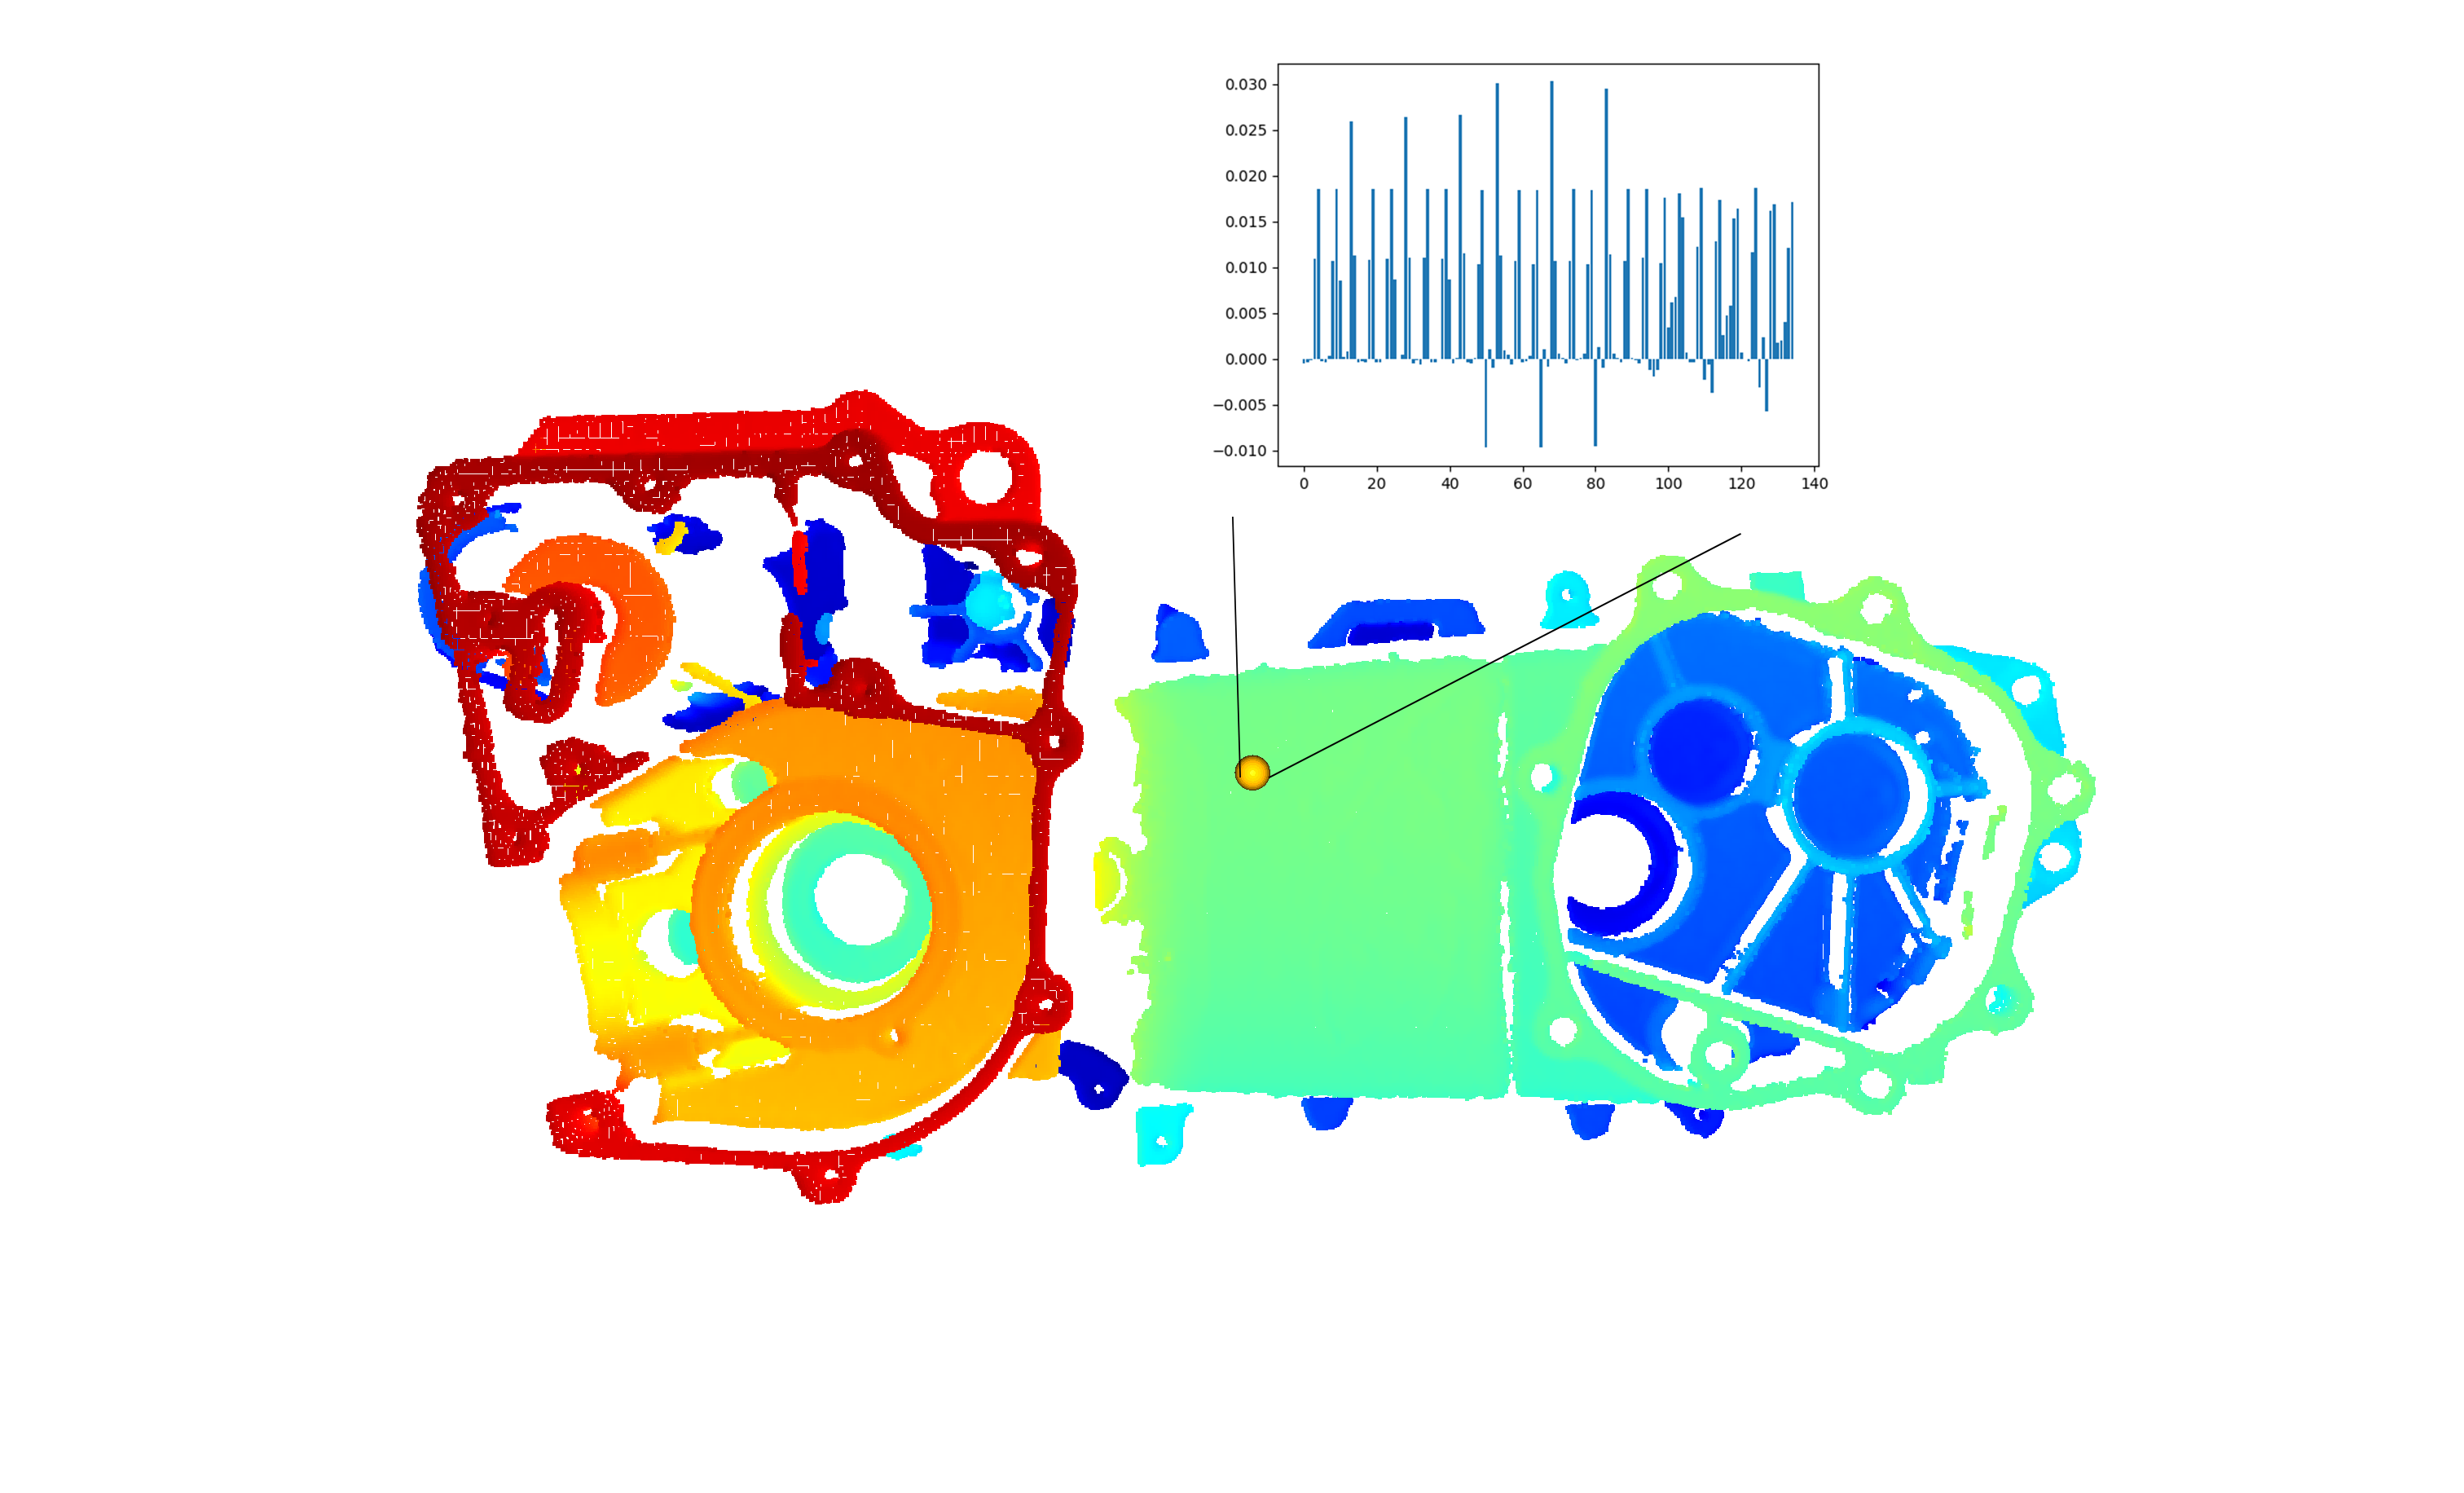
\includegraphics[width=1\textwidth]{figures/RoPS_and_histogram.png}
    \caption{RoPS描述子}
    \label{fig:RoPS_and_histogram}
\end{figure}

\section{三维缺陷检测}
PatchCore是应用在二维RGB图像上且表现出优异性能的无监督缺陷检测算法。PatchCore使用预训练网络对正常样本提取特征然后按块进行聚合到特征存储体并通过核心集降采样加快推理速度,最终通过测试数据的聚合特征与存储体最近邻距离输出异常得分。

本文通过结构光相机采集的点云数据实际上是2.5D数据,沿Z轴投影点云并经过插值等处理后即可生成深度图像,其通道为拍摄物到相机的距离。因此对于有序点云,经过标定对齐后,其x、y的值和其对应RGB图像的坐标一致,从而可以迁移PatchCore的方法,本文称基于PatchCore思想应用于点云的算法为PillarCore。
\subsection{柱特征}
本文用 $\mathcal{X}_{N}$定义所有训练时用的正常点云样本集 $\left(\forall x\in \mathcal{X}_{N}: y_{x}=0\right)$,用 $\mathcal{X}_{T}$定位测试时的点云样本集,用$y_{x} \in\{0,1\}$定义点云样本 $x$类型,其中(0)表示正常样本,(1)表示异常样本。类似于PatchCore将二维图像划分为块(Patch),本文的PillarCore将点云像切蛋糕一样划分为柱(Pillar)。

假设点云 $x_{i} \in \mathcal{X}$( $\mathcal{X}$为数据集)的特征 $\phi_{i} \in \mathbb{R}^{c^{*} \times h^{*} \times w^{*}}$是有 $c^{*}$ 深度$h^{*}$高度 $w^{*}$宽度的三维张量。用 $\phi_{i}(h, w)=\phi\left(x_{i}, h, w\right) \in \mathbb{R}^{c^{*}}$定义在位置 $h \in \{1,…,h^{*}\}$和 $w \in \{1,…,w^{*} \}$ 的$c^{*}$维RoPS特征描述子。

为了增加算法的鲁棒性同时不损失空间分辨率,在组成每个柱级特征表征时进行局部邻域聚合。来自邻域的特征向量按式\ref{equ:nphw} 定义 。

\begin{equation}\label{equ:nphw}
    \begin{aligned}\mathcal{N}_{p}^{(h, w)}=\{(a, b) \mid a & \in[h-\lfloor p / 2\rfloor, \ldots, h+\lfloor p / 2\rfloor], \\b & \in[w-\lfloor p / 2\rfloor, \ldots, w+\lfloor p / 2\rfloor]\},\end{aligned}
\end{equation}


在位置$(h,w)$的局部特征表示如式\ref{equ:aggf},其中$f_{\mathrm{agg}}$聚合邻域 $\mathcal{N}_{p}^{(h, w)}$里的特征向量。

\begin{equation}\label{equ:aggf}
    \phi_{i}\left(\mathcal{N}_{p}^{(h, w)}\right)=f_{\mathrm{agg}}\left(\left\{\phi_{i}(a, b) \mid(a, b) \in \mathcal{N}_{p}^{(h, w)}\right\}\right)
\end{equation}

对于特征张量 $\phi_{i}$,其局部特征集 $\mathcal{P}_{s, p}\left(\phi_{i}\right)$按式\ref{equ:localfeat}定义,其中步长参数 s 是可选的,一般设置为1。

\begin{equation}\label{equ:localfeat}
    \mathcal{P}_{s, p}\left(\phi_{i}\right)=\left\{\phi_{i}\left(\mathcal{N}_{p}^{(h, w)}\right) \mid\right.
 \left.h, w \bmod s=0, h<h^{*}, w<w^{*}, h, w \in \mathbb{N}\right\} 
\end{equation}

最后,对所有正常训练样本 $x_{i} \in \mathcal{X}_{N}$,本文参考PatchCore提出的块级特征存储体,针对点云数据建立了柱级特征存储体 $\mathcal{M}$,如式\ref{equ:memorybank} 所示。

\begin{equation}\label{equ:memorybank}
    \mathcal{M}=\bigcup_{x_{i} \in \mathcal{X}_{N}} \mathcal{P}_{s, p}\left(\phi_{j}\left(x_{i}\right)\right)
\end{equation}

\subsection{核心集降采样}
对持续增长的$\mathcal{X}_{N}$,$\mathcal{M}$变得非常大,因此评估新测试数据的推断时间和所需的存储量都会增加。随机二次抽样从一定程度上能解决问题,但几个数量级的抽样将丢失在正常样本特征覆盖范围内编码的$\mathcal{M}$中可用的重要信息。本文采用PatchCore提出的核心集降采样机制来减少$\mathcal{M}$ ,这样可以在保持性能的同时减少推理时间。

理论上,核心集选择的目的是找到子集 $\mathcal{S} \subset \mathcal{A}$,使得在A上的问题求解能最接近,特别是更快速地逼近在S上计算求解。根据具体问题,关注的核心集有所不同。Patchcore由于使用最近邻计算,其选择使用一种极小极大设施选址(minimax facility location) 算法进行核心集选择,如式\ref{equ:mdown}所示,来确保与原始存储体$\mathcal{M}$ 相比,$\mathcal{M}$ 的核心集$\mathcal{M}_c$ 在块级特征空间的覆盖率大致相似。

\begin{equation}\label{equ:mdown}
    \mathcal{M}_{C}^{*}=\underset{\mathcal{M}_{C} \subset \mathcal{M}}{\arg \min } \max _{m \in \mathcal{M}} \min _{n \in \mathcal{M}_{C}}\|m-n\|_{2} .
\end{equation}

$\mathcal{M}_{C}^{*}$的精确计算是NP-HARD问题。PatchCore使用迭代贪婪近似,来进一步减少核心集的选择时间。利用Johnson-Lindenstrauss定理,通过随机线性投影 $\psi: \mathbb{R}^{d} \rightarrow \mathbb{R}^{d^{*}}$   ,其中 $d^{*}<d$  来减少元素 $m \in \mathcal{M}$的维度。

% 存储体的降维总结为伪代码。


\subsection{缺陷检测}
建立正常样本块特征存储体后,PatchCore通过测试图像 $x^{test}$的块集合 $\mathcal{P}\left(x^{\text {test }}\right)=\mathcal{P}{s, p}\left(\phi{j}\left(x^{\text {test }}\right)\right)$中测试块特征和$\mathcal{M}$ 中的每个最近邻 $m^{*}$之间的最大距离分数 $s^{*}$,对测试图像 $x^{test}$估计图像级异常分数 $s \in \mathbb{R}$ 。其中$s^{*}$的计算公式如式\ref{equ:sstar}所示。

\begin{equation}\label{equ:sstar}
    \begin{aligned}m^{\text {test }, *}, m^{*} & =\underset{m^{\text {test }} \in \mathcal{P}\left(x^{\text {test })}\right)}{\arg \max } \underset{m \in \mathcal{M}}{\arg \min }\left\|m^{\text {test }}-m\right\|_{2} \\s^{*} & =\left\|m^{\text {test }, *}-m^{*}\right\|_{2} .\end{aligned}
\end{equation}


PatchCore通过使用$s^{*}$上的缩放因子w来表示相邻块的关系从而计算s,如式\ref{equ:score}所示。如果最接近异常候选 $m^{\text {test},* }$, $m^{*}$的存储体特征本身远离相邻样本,即很少出现的正常样本,缩放因子会使异常分数增加。

\begin{equation}\label{equ:score}
    s=\left(1-\frac{\exp \left\|m^{\text {test }, *}-m^{*}\right\|_{2}}{\sum_{m \in \mathcal{N}_{b}\left(m^{*}\right)} \exp \left\|m^{\text {test }, *}-m\right\|_{2}}\right) \cdot s^{*}
\end{equation}

其中 $\mathcal{N}_{b}\left(m^{*}\right)$ 是$\mathcal{M}$ 中离测试块特征 $m^{*}$最近的b个块特征。这种重新加权比最大块距离更鲁棒。图像级异常的分需要通过对每个块进行arg max运算得出。此外,还可在同一步骤中计算分割图,通过基于他们各自空间位置调整计算的异常得分。

PatchCore的核心集降采样和异常得分计算都是在进行特征聚合后,而本文所研究的点云数据在经过柱特征抽象后与二维RGB图像块特征抽象后的表现形式相近,因此本文的PillarCore直接复用其后续流程方法,实现点云数据的缺陷检测。

\section{实验设计及结果分析}
\subsection{数据集}
本文被检对象为实验室的摩托车金属件,该金属件结构复杂,最小外接立方体的长宽高为$0.52m\times 0.22m \times 0.09m$,其XY方向点云标量图如图\ref{fig:pcdxy}所示。
\begin{figure}[htbp]
    \centering
    \begin{subfigure}
        \centering
        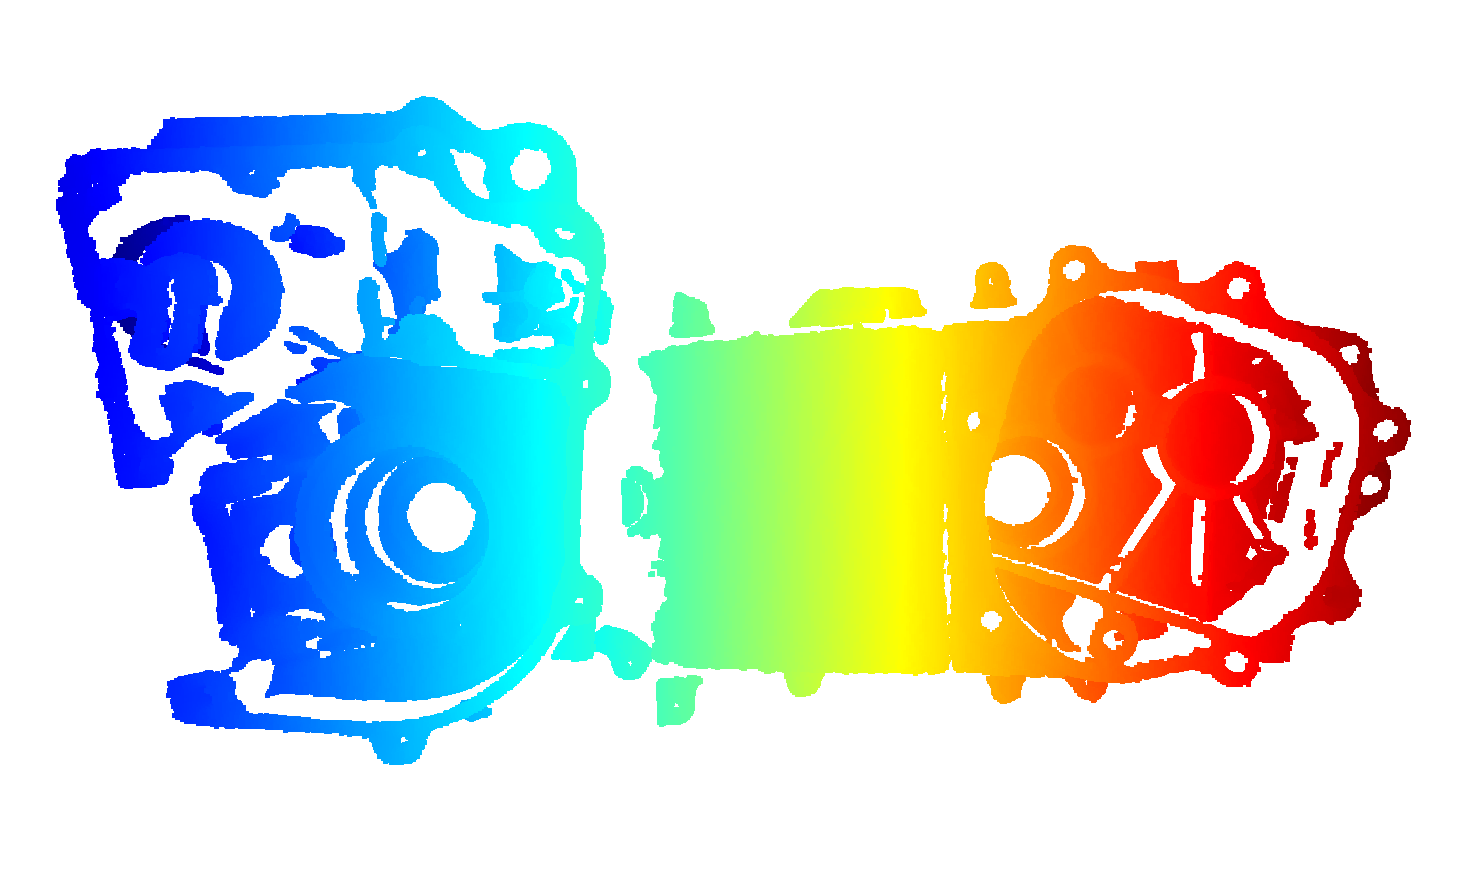
\includegraphics[width=.4\linewidth]{figures/3/normal-x.png}  
      \end{subfigure}
      \begin{subfigure}
        \centering
        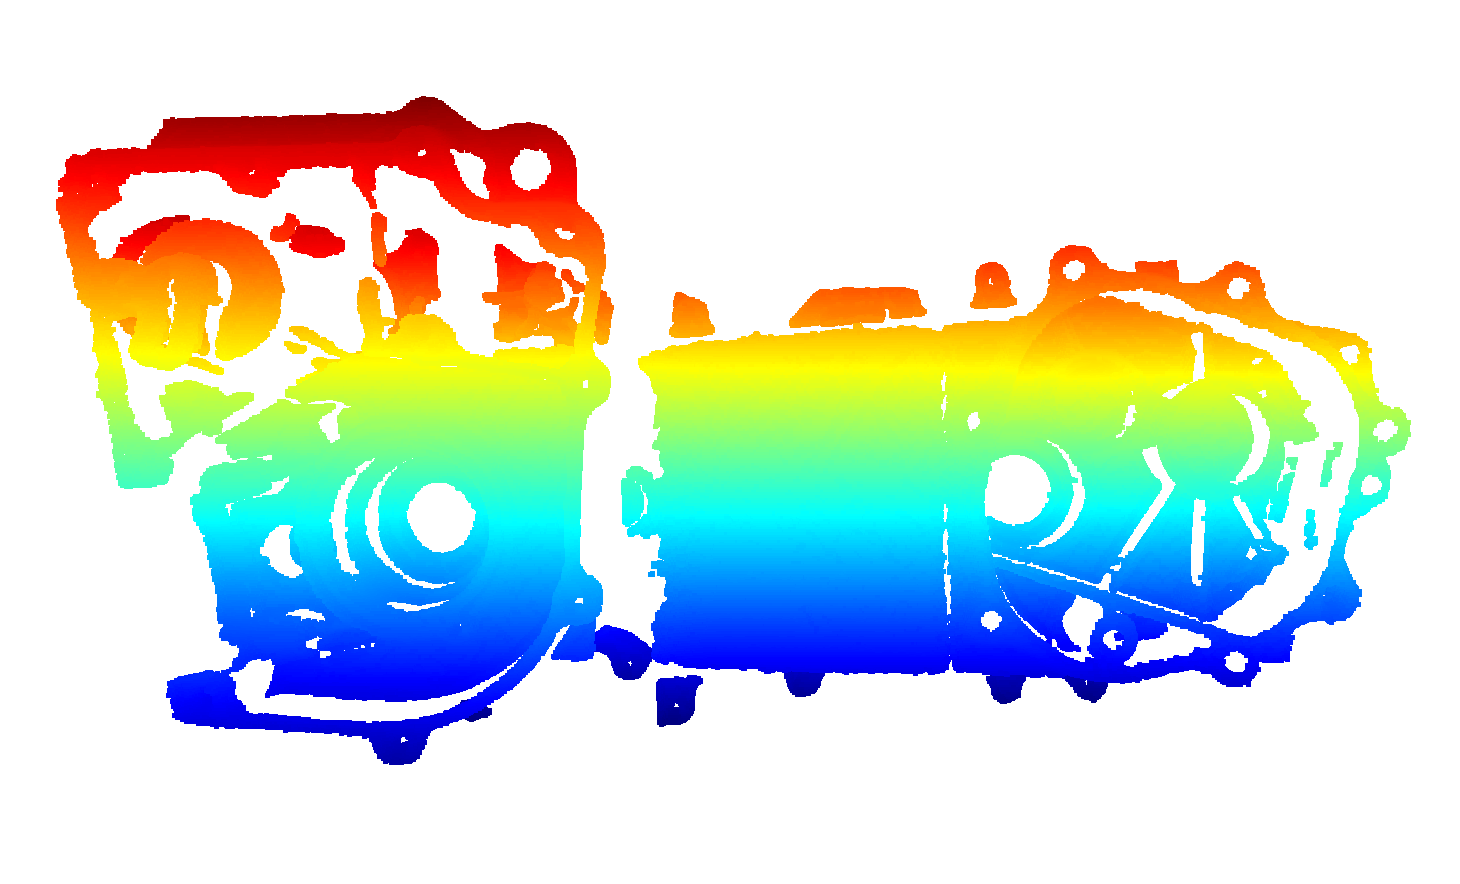
\includegraphics[width=.4\linewidth]{figures/3/normal-y.png} 
      \end{subfigure}
    \caption{采集点云数据XY标量图}
    \label{fig:pcdxy}
  \end{figure}

本文使用第二章搭建的实验平台对金属件进行拍摄,采集正常样本和手工制造的缺陷样本的点云数据制作数据集。其中训练数据集全部为正常样本,测试数据集由结构缺陷和正常样本共同组成。部分正常样本和缺陷样本如图\ref{fig:normalxy}和图\ref{fig:bad}所示。其中图\ref{fig:normalxy}中的正常样本是对同一工件从多个角度采集的。图\ref{fig:bad}中红色框表示缺陷样本缺陷处俯视和侧视两个角度的视图。侧视视角中,红框范围内绿色部分点云为缺陷样本中的一个结构缺陷。

  \begin{figure}[htbp]
    \centering
    \begin{subfigure}
        \centering
        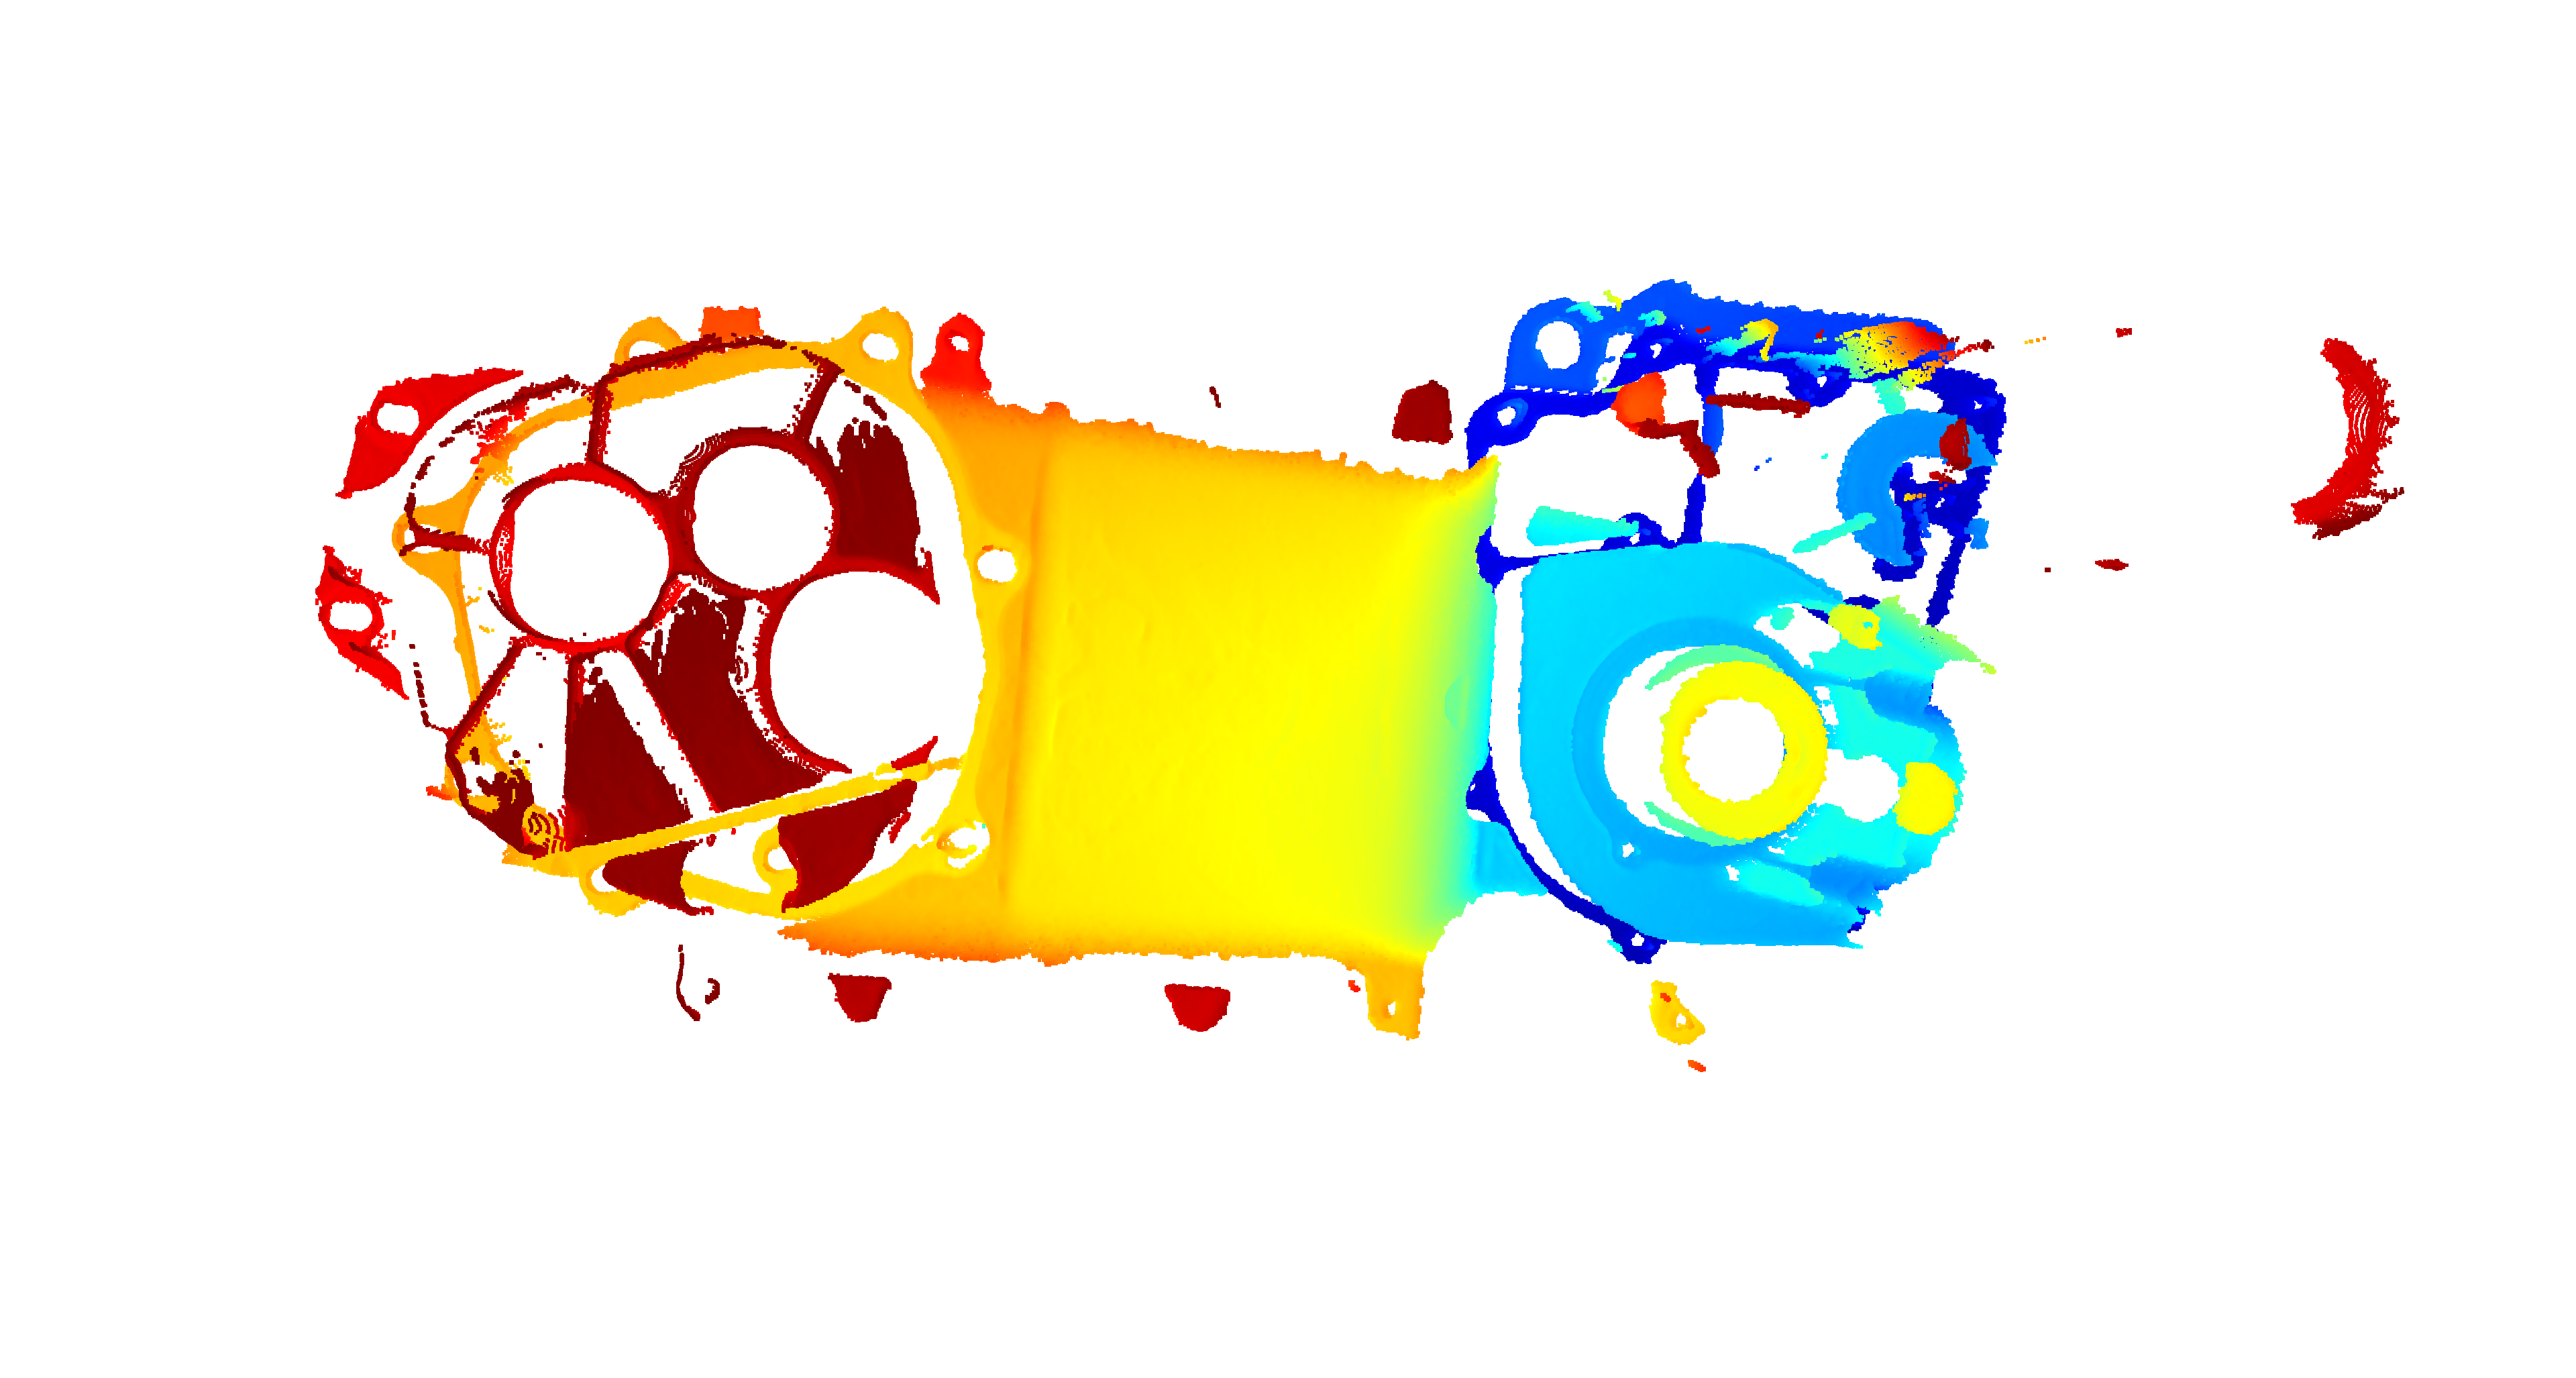
\includegraphics[width=.4\linewidth]{figures/3/good-1.png}  
      \end{subfigure}
      \begin{subfigure}
        \centering
        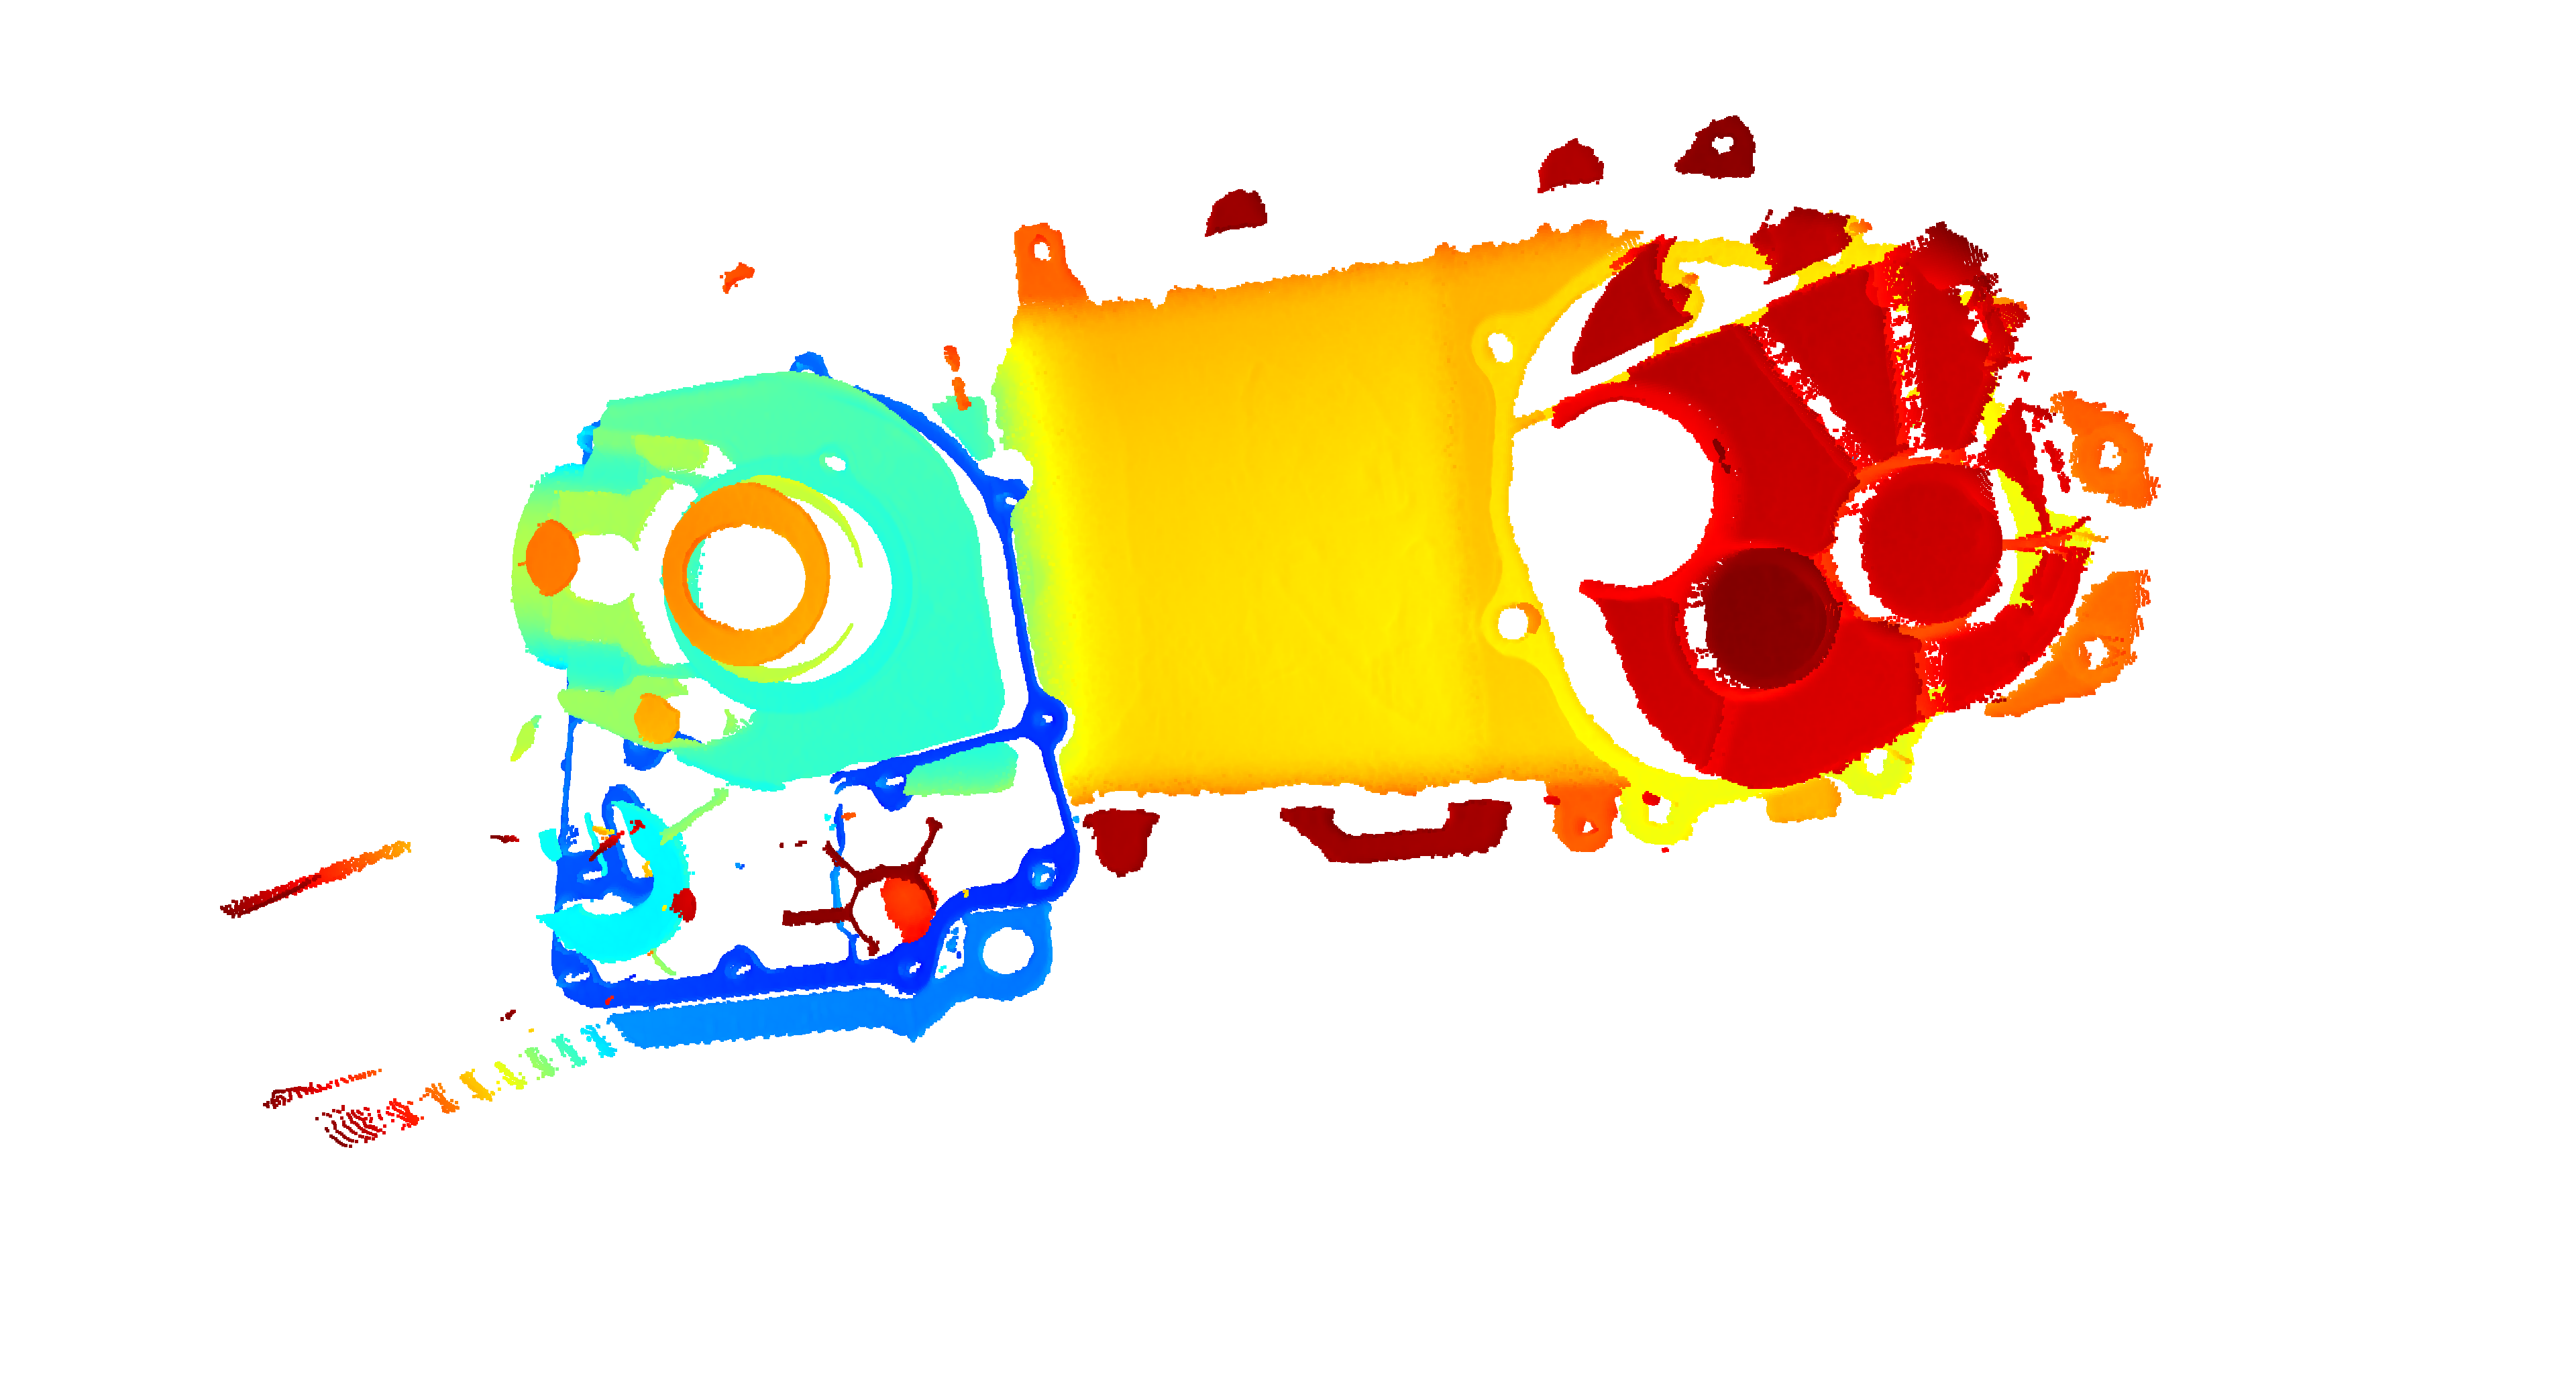
\includegraphics[width=.4\linewidth]{figures/3/good-2.png} 
      \end{subfigure}
      \begin{subfigure}
        \centering
        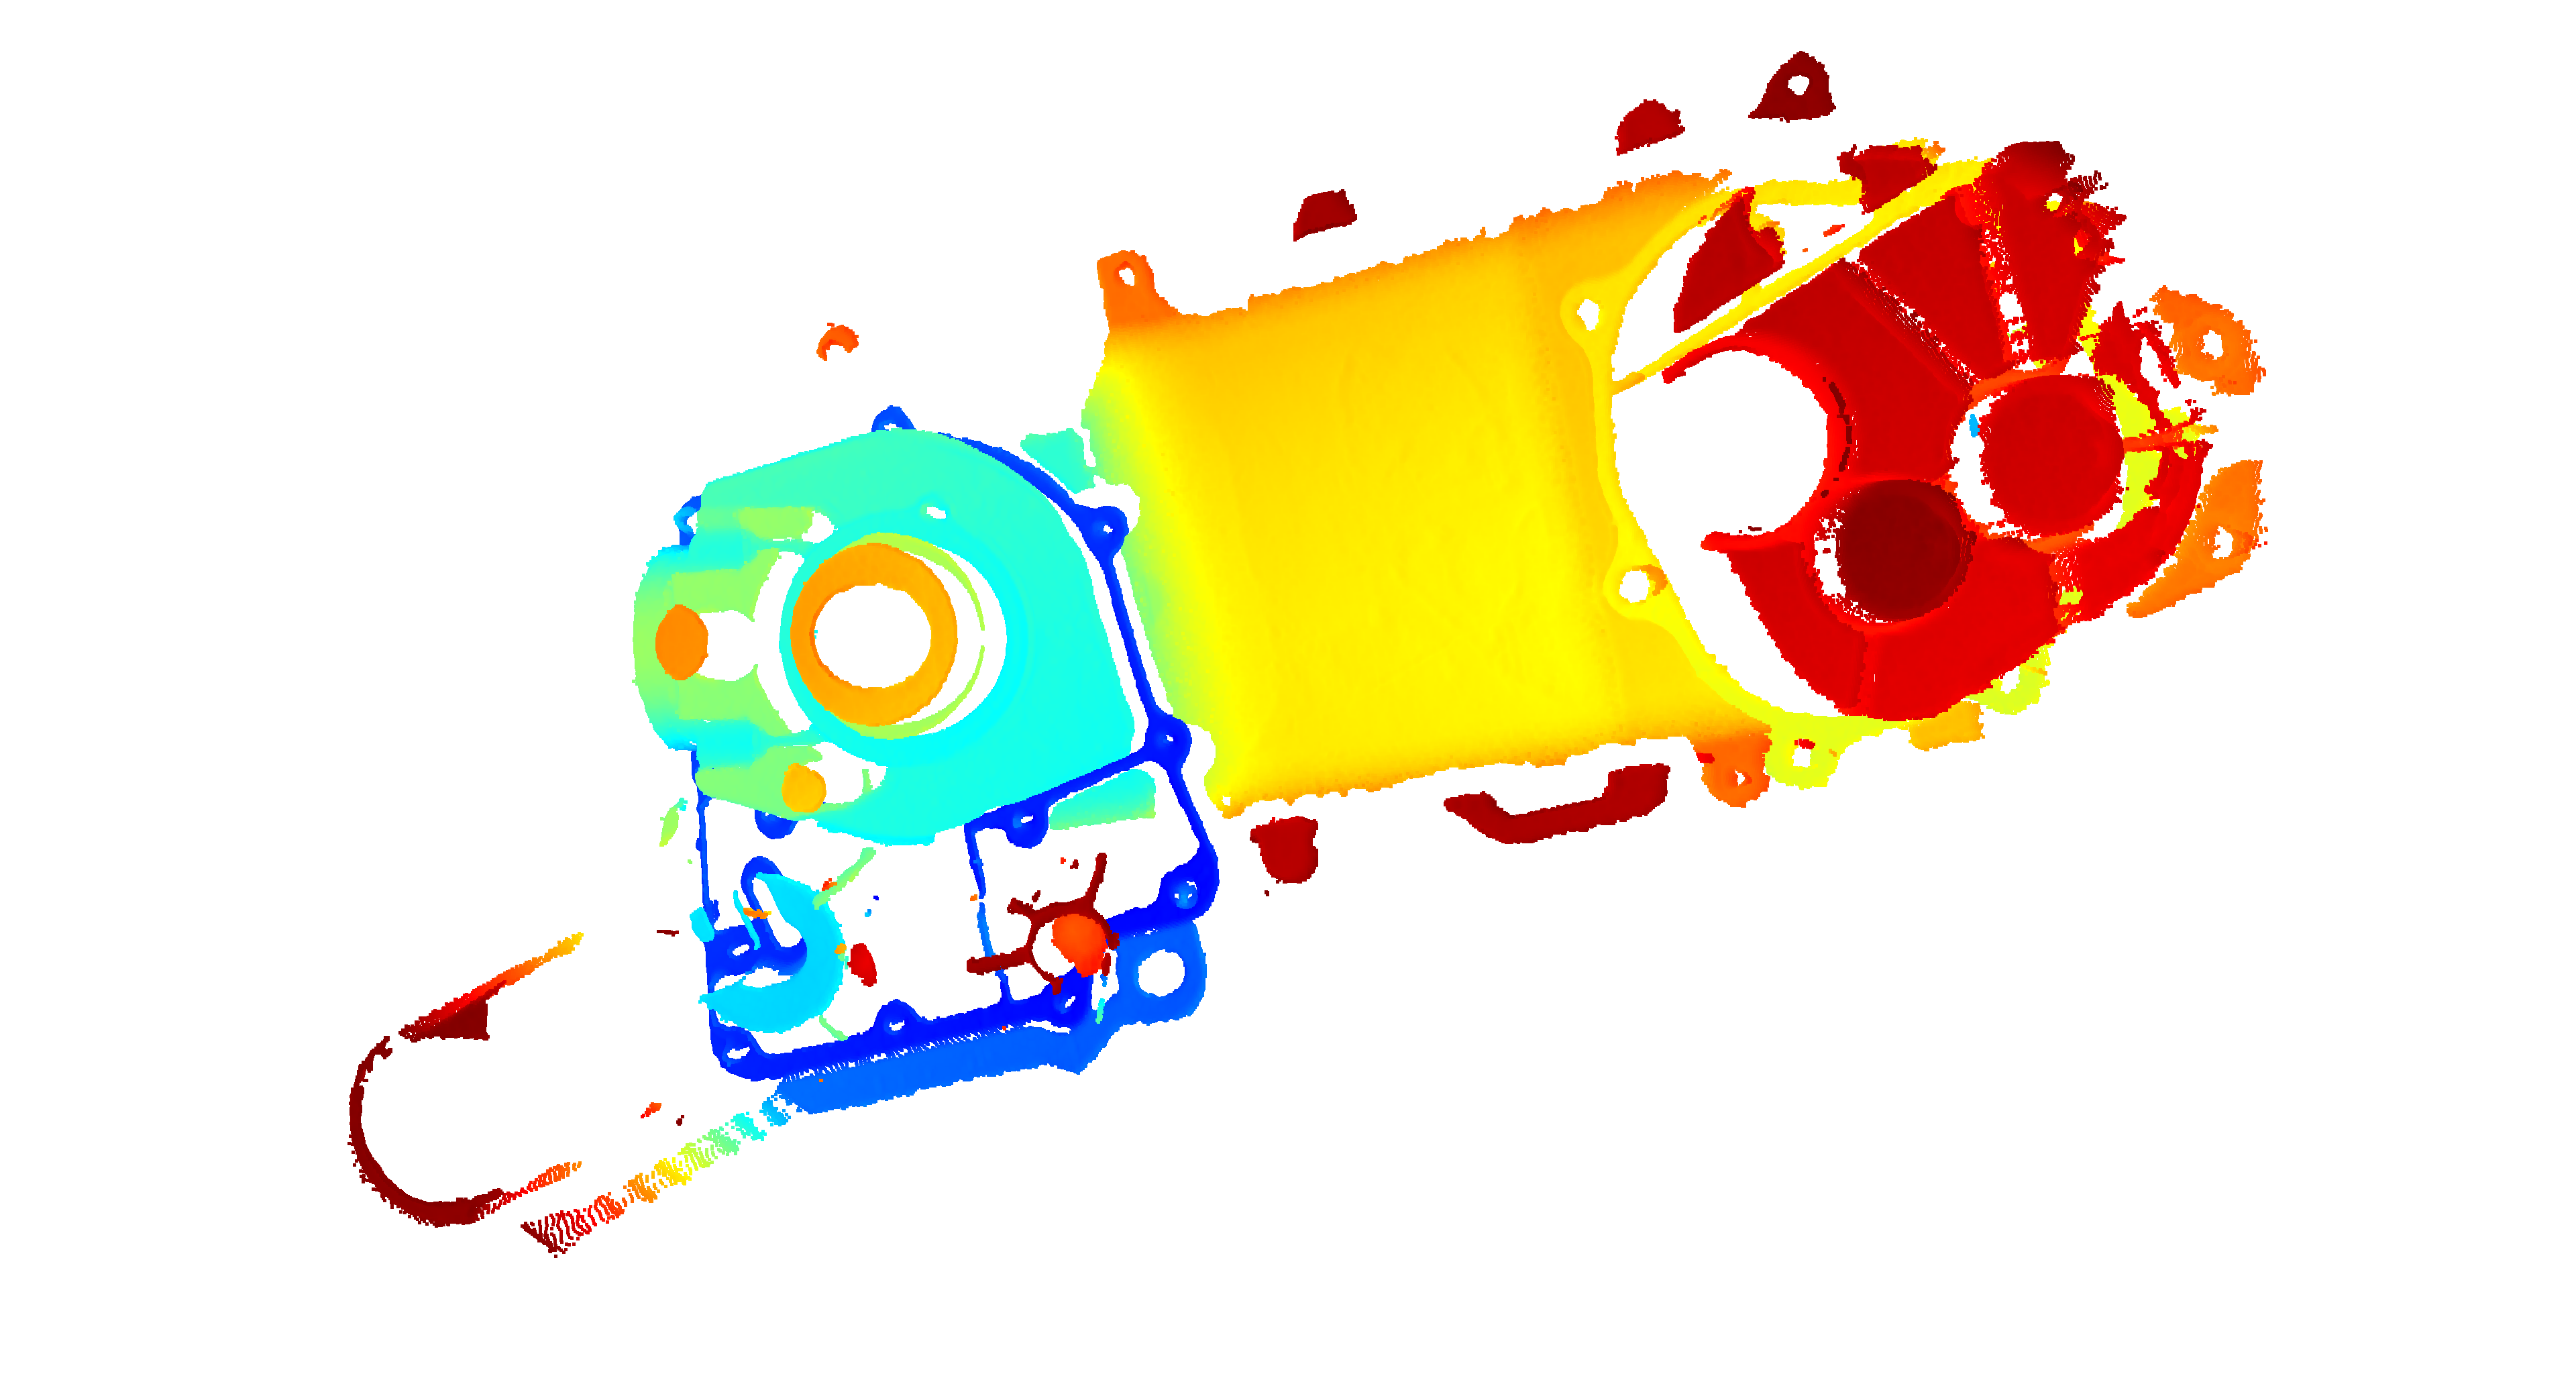
\includegraphics[width=.4\linewidth]{figures/3/good-3.png}  
      \end{subfigure}
      \begin{subfigure}
        \centering
        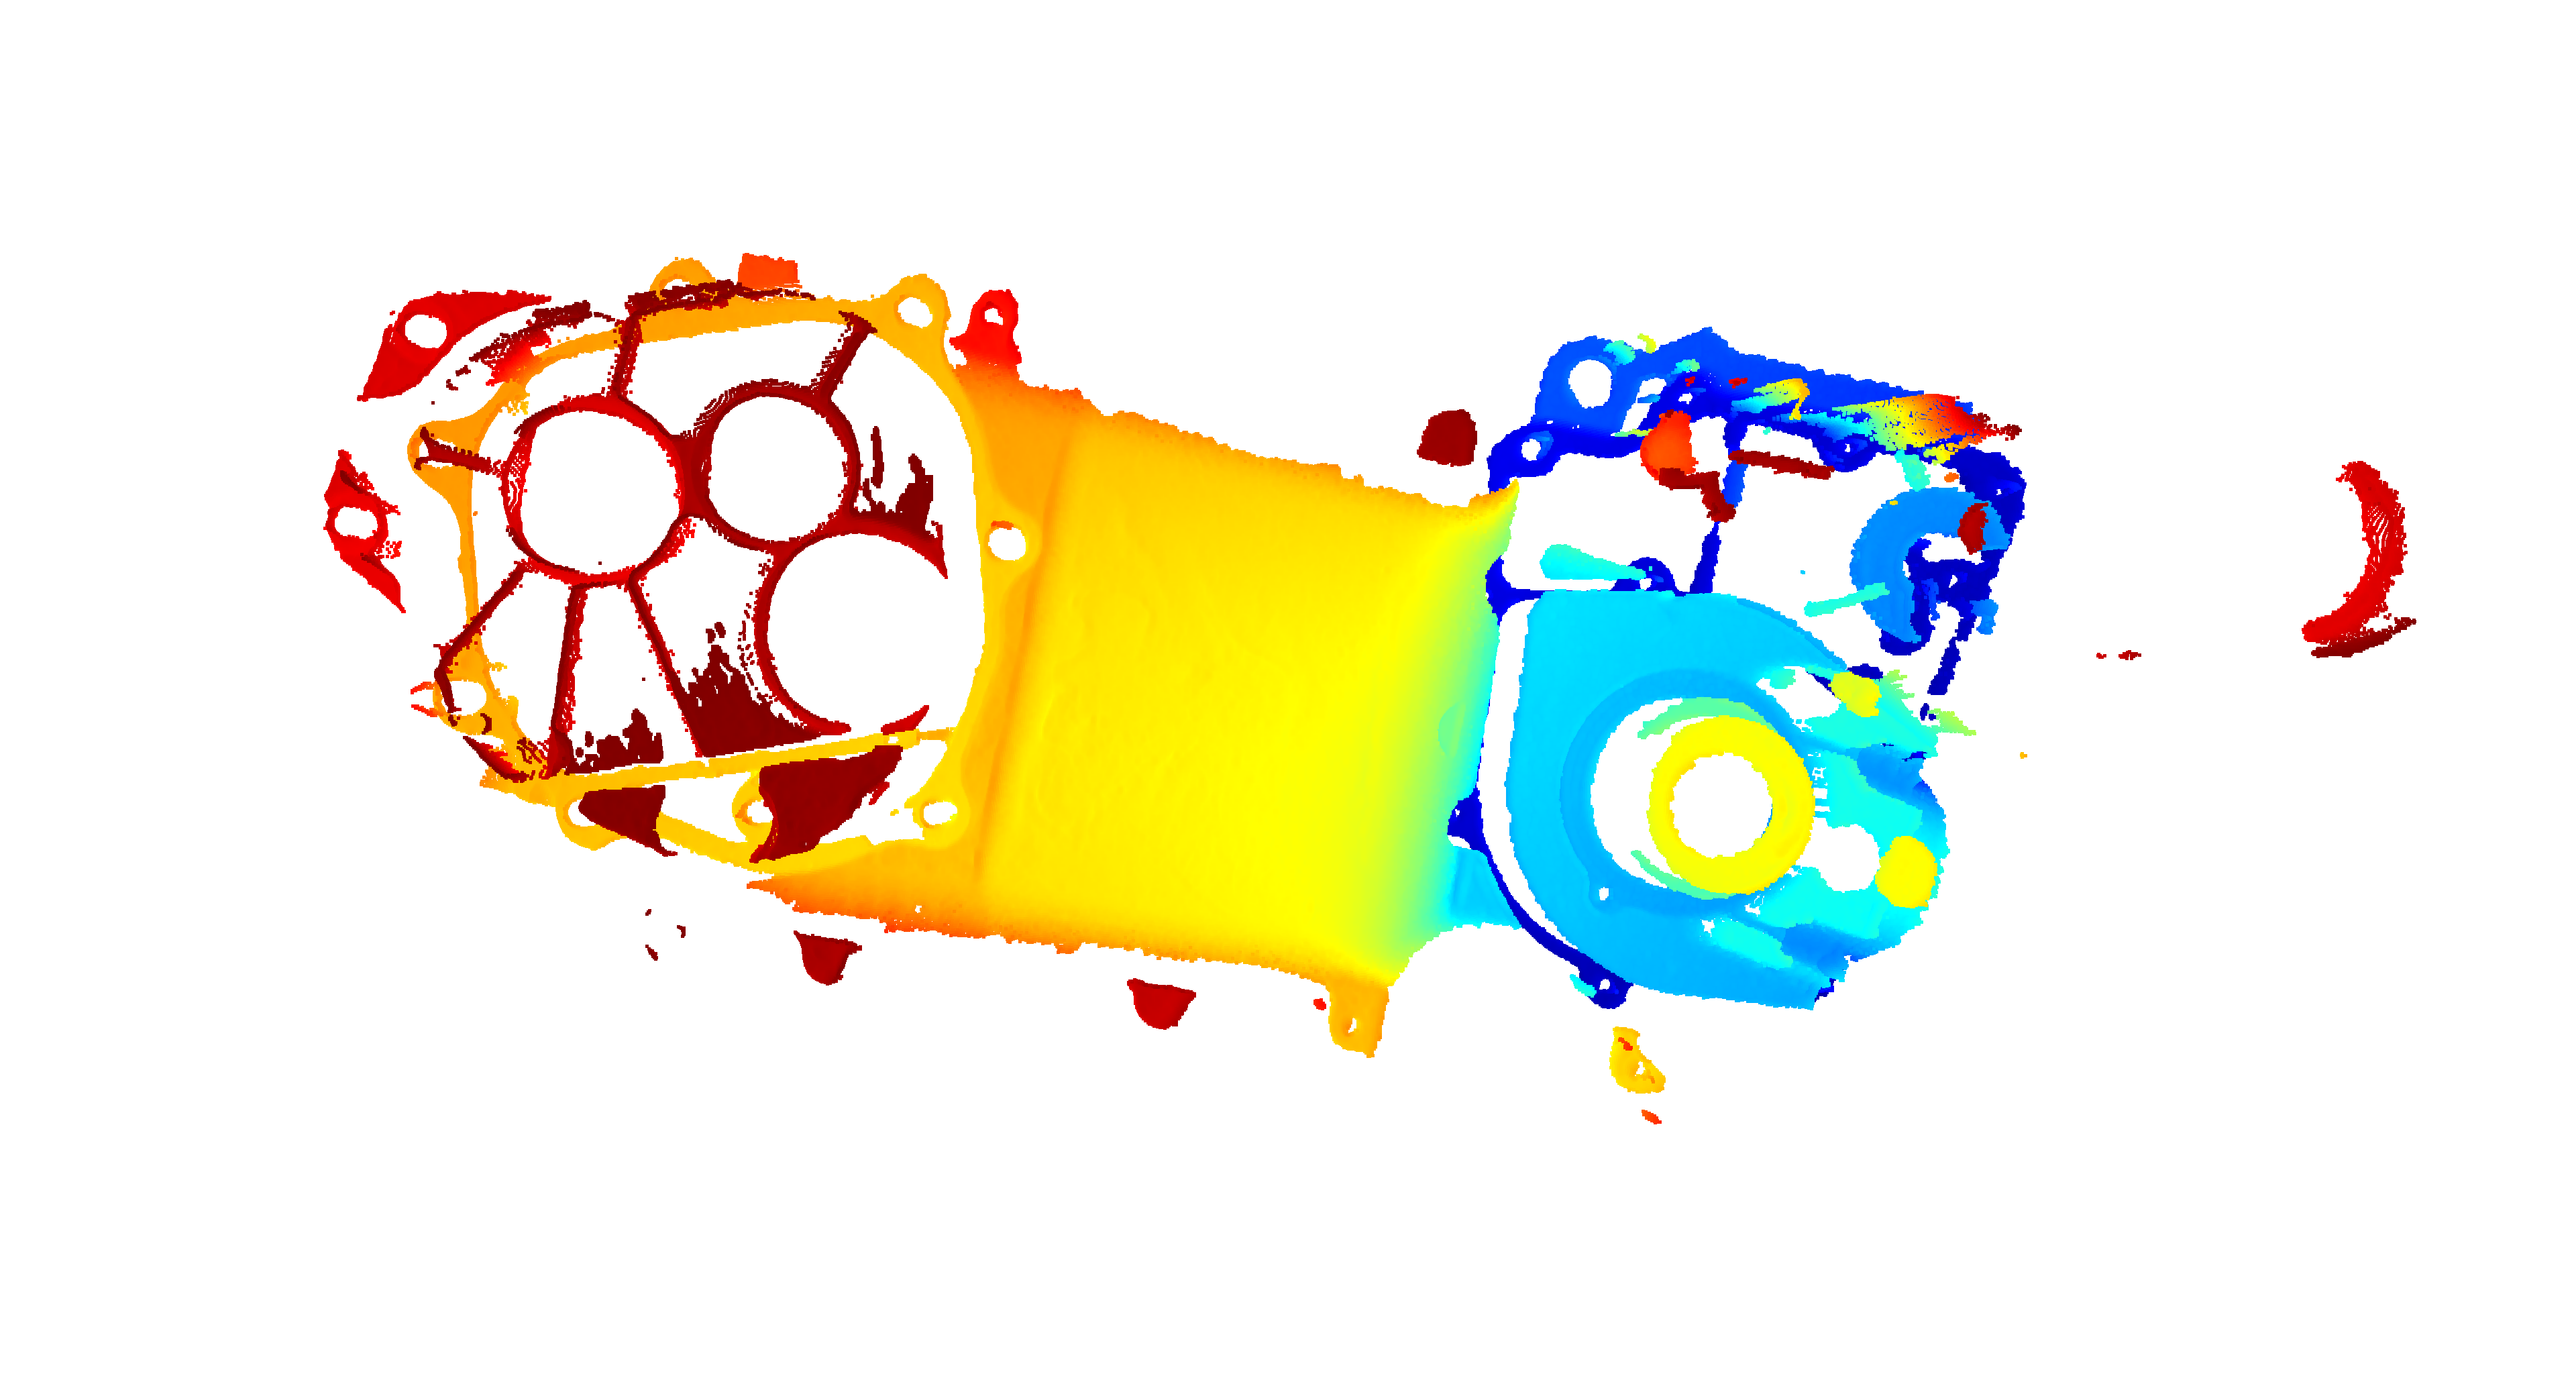
\includegraphics[width=.4\linewidth]{figures/3/good-4.png} 
      \end{subfigure}
    \caption{部分正常样本}
    \label{fig:normalxy}
  \end{figure}

  \begin{figure}[htbp]
    \centering
    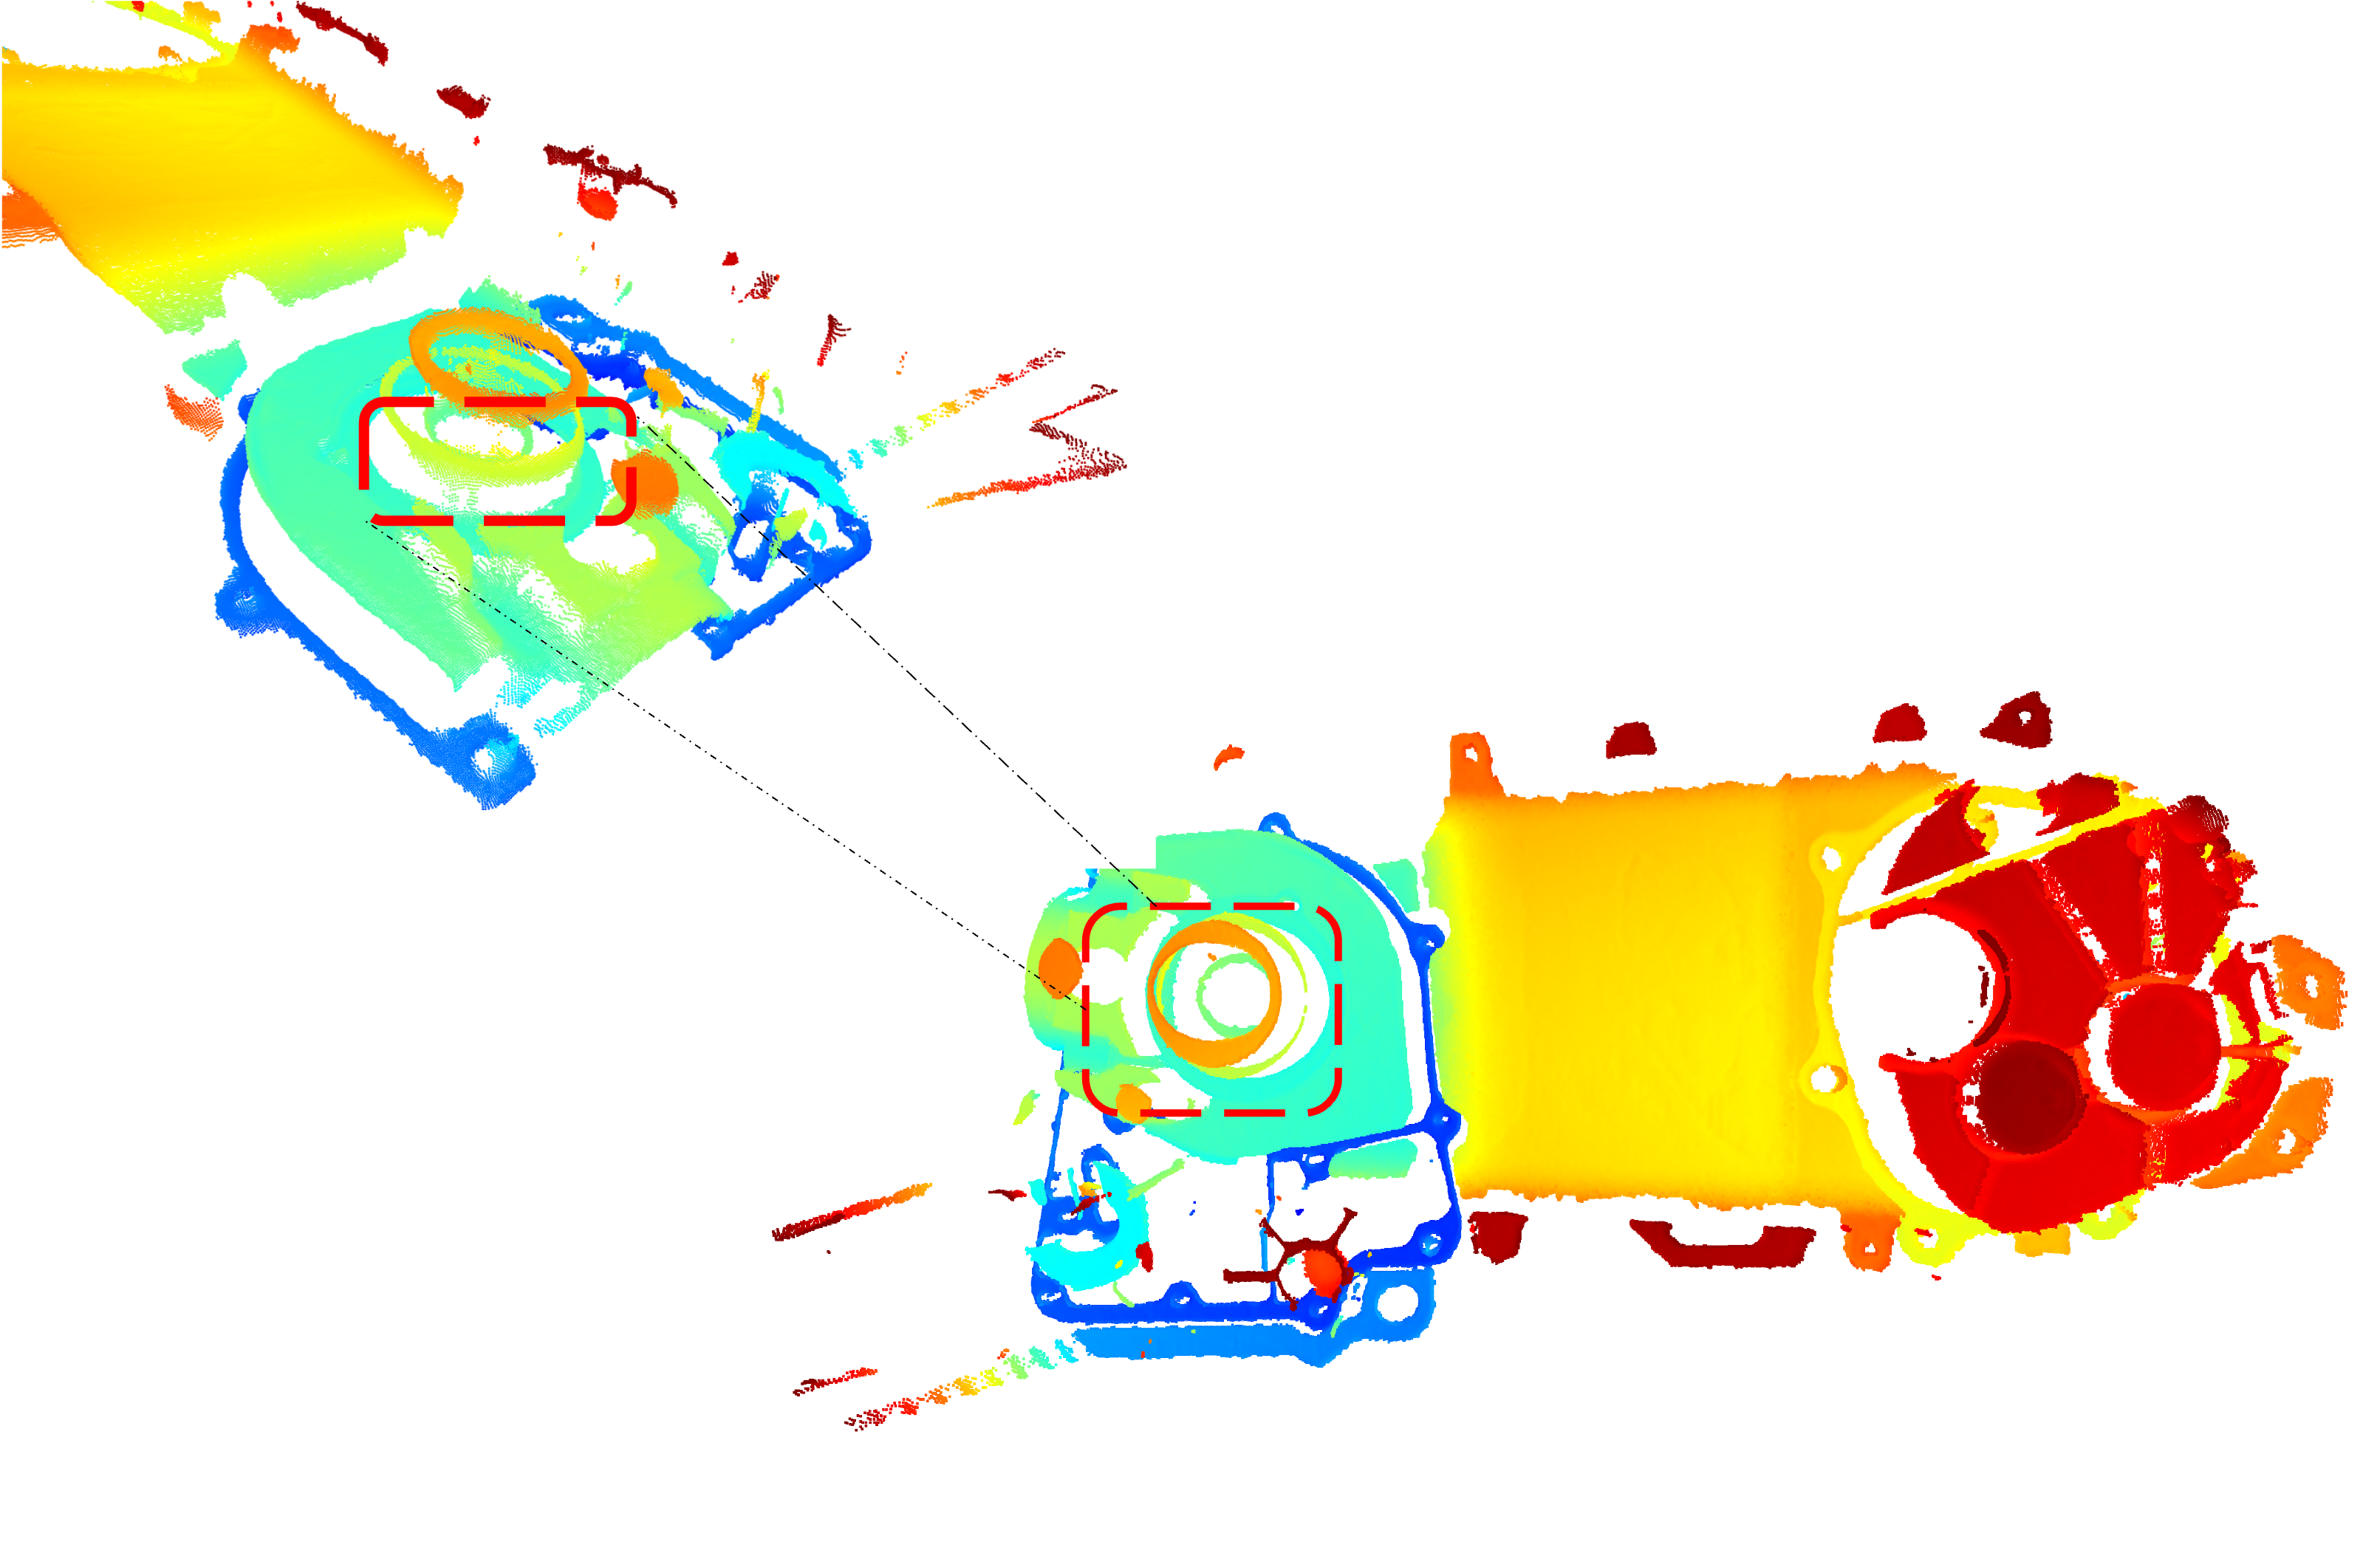
\includegraphics[width=0.75\textwidth]{figures/3/bad.png}
    \caption{结构缺陷样本示例}
    \label{fig:bad}
\end{figure}

此外,本文还引入了公开的3D缺陷检测数据集MVTec3D-AD\cite{bergmannMVTec3DADDataset2022},其包含有10种类型物体的训练和测试数据集。

\subsection{实验设计}
本文在Patchcore基础上引入的3D局部特征描述子RoPS是基于空间分布直方图来提取3D特征的,而3D局部特征描述子还有另一类是基于几何属性直方图的,其中以FPFH(Fast Point Feature Histograms)方法最为广泛应用,该方法将每个点的几何信息(例如,法线、曲率)和邻域关系转换为直方图表示。

因此本文以FPFH为基准设计对比实验,如表\ref{tab:3-experiment-desgin}所示。其中FPFH的直方图维数为,RoPS直方图的维数为135,两者均应用于点云降采样后的所有点。
\begin{table}[htbp]
    \centering
    \caption{金属工件数据集实验设计} \label{tab:3-experiment-desgin}
    \begin{tabular*}{0.6\textwidth}{@{\extracolsep{\fill}}ccc}
    \toprule
      &原理&直方图维数\\
      \midrule
        FPFH&几何属性&33\\
        RoPS	&空间分布&135\\
    \bottomrule
    \end{tabular*}
\end{table}

\subsection{实验结果和分析}
本文按照实验设计在正常样本组成的训练集上分别采用FPFH和RoPS提取3D特征并通过PillarCore聚合存储后,在自建的数据集和公开数据集上验证了算法的性能。实验采用的评价指标为在第二章中介绍的图像级的AUROC,其中在本文的金属件数据集上的实验结果如表\ref{tab:motor-experiment}所示。
\begin{table}[htbp]
    \centering
    \caption{金属工件数据集图像级AUROC} \label{tab:motor-experiment}
    \begin{tabular*}{0.4\textwidth}{@{\extracolsep{\fill}}cc}
    \toprule
      &金属工件\\
      \midrule
        FPFH&0.929\\
        RoPS	&0.96\\
    \bottomrule
    \end{tabular*}
\end{table}

从金属工件数据集实验结果中不难看出,本文引入RoPS作为3D局部特征提取提子的方法在本文的金属工件上的性能要优于FPFH方法。

\begin{table}[htbp]
    \centering
    \caption{MVTec3D-AD数据集图像级AUROC} \label{tab:mvtec3d-experiment}
    \begin{tabular*}{1\textwidth}{@{\extracolsep{\fill}}ccccccccccc}
    \toprule
      &百吉圈&密封套&萝卜&曲奇&暗榫&泡沫板&桃&土豆&绳索&轮胎\\
      \midrule
        FPFH&0.82&0.533&0.877&0.769&0.718&0.574&0.774&0.895&0.99&0.582\\
        RoPS&$\mathbf{0.868}$&$\mathbf{0.534}$&0.565&$\mathbf{0.989}$&$\mathbf{0.774}$&$\mathbf{0.692}$&0.77&0.819&0.834&0.577\\
    \bottomrule
    \end{tabular*}
\end{table}

在MVTec3D-AD数据集上的实验结果如表\ref{tab:mvtec3d-experiment}所示,其中黑色加粗表示在百吉圈、密封套、曲奇、暗榫以及泡沫板数据集上,本文引入RoPS的方法比FPFH的方法图像级AUROC指标高。从曲奇和萝卜两个数据集的图像级AUROC指标可以看出,基于空间分布的RoPS方法和基于几何分布的FPFH方法有各自擅长的点。两种方法在曲奇数据集上的ROC曲线如组图\ref{fig:cookie}所示,其中左图为FPFH方法,右图为RoPS方法。

\begin{figure}[htbp]
    \centering
    \begin{subfigure}
        \centering
        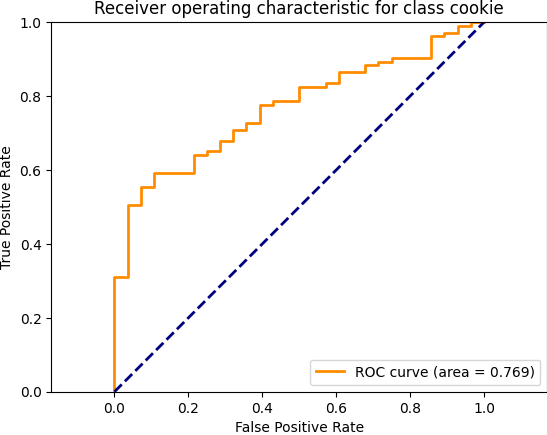
\includegraphics[width=.42\linewidth]{figures/3/cookie_FPFH.png}  
      \end{subfigure}
      \begin{subfigure}
        \centering
        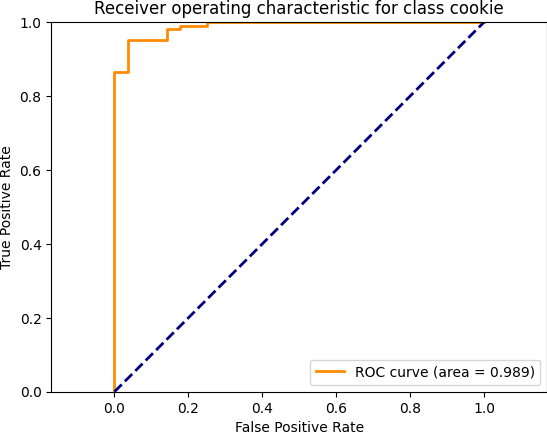
\includegraphics[width=.42\linewidth]{figures/3/cookie_RoPS.png} 
      \end{subfigure}
    \caption{曲奇数据集ROC曲线图}
    \label{fig:cookie}
  \end{figure}

\section{本章小结}
本章分别分别从整体算法框架、算法的输入处理方法(包括点云预处理、点云三角化及点云局部特征提取)和算法的核心处理方法三个角度介绍了本文提出的基于点云的面向非平整表面无监督缺陷检测算法PillarCore——通过引入RoPS特征提取方法将应用于二维图像缺陷检测的PatchCore方法迁移到三维数据,并在多个数据集和FPFH算法的对比实验中验证了本方法的有效性。


\chapter{基于多模态的缺陷检测}

\section{多模态缺陷检测框架}
3D数据在检测结构缺陷上具有优势,而RGB图像对于纹理缺陷则更有优势。当面对可能同时具有结构和纹理缺陷的场景,综合利用3D数据和RGB图像能够取得更好的效果。其中由于RGB数据的表现形式是二维图像,因此本文选择使用同样为二维图像的深度图作为3D数据与RGB数据融合作为输入,从而实现多模态的缺陷检测算法。

本文采用异构教师学生网络(AST)\cite{rudolphAsymmetricStudentTeacherNetworks2022}作为多模态缺陷检测的骨干网络。AST目标是训练两个异构的模型,一个记作学生模型$f_{s}$,另一个一个记作教师模型$f_{t}$。其中学生只根据无缺陷的正常样本来回归教师网络的输出,其假设在正常样本上训练的教师学生网络在缺陷样本上有较大差异。整个训练过程分为两个阶段:

首先是训练教师网络模型,本文利用标准化流将训练数据分布$p_{X}$通过双射变换函数转换为正态分布N(0,I)。然后,通过最小化训练样本 $x \in X$的 $f_{s}(x)$和$f_{t}(x)$之间的距离,优化学生网络来匹配教师网络的输出。最后,在测试网络性能时,利用教师学生之间的距离计算异常评分。

本文不直接将RGB图像输入骨干网络,而是利用在ImageNet上预训练的网络模型作为通用特征提取器,对图像进行特征提取后再输入。对于深度图像,本文引入HOG特征描述子来进行深度特征提取,其特征维度与RGB的特征图相匹配,从而方便后续融合。在提取特征前,本文利用多模态的优势,通过深度图像的前景提取来创建蒙版,并用于RGB图像前景提取和后续的距离损失计算,相比于单独使用RGB图像,有效降低了计算量并且提升了性能。
\begin{figure}[htbp]
    \centering
    \includegraphics[width=1\textwidth]{figures/4/framework.pdf}
    \caption{多模态缺陷检测框架}
    \label{fig:4-framework}
\end{figure}

此外,为应对与位置相关的缺陷,本文还采用位置编码的方法来对输入特征图的进行位置编码,并用于学生和教师网络。本文的多模态缺陷检测整体框架如图\ref{fig:4-framework}所示



\section{多模态输入预处理}
\subsection{RGB和深度图像对齐}
RGB 图像在深度学习中被广泛用于各种任务。RGB 图像具有红色(R)、绿色(G)和蓝色(B)三个通道,每种通道都有一个从 0 到 255 的值,其中 0 表示没有颜色,255 表示全色。通过这三个通道可以表示图像的不同特征。不过RGB 图像在计算机视觉任务中也有一些局限性。例如,RGB 图像对光照变化、遮挡和阴影很敏感。 RGB 图像也可能无法区分具有相似颜色或形状的对象。

为了克服这些挑战,在视觉任务的实际应用中,一些方法会在RGB图像的基础上在引入更直观表现深度信息的深度图像,组合成RGB-D 图像。由于深度测量相机可以直接计算与图像中每个像素之间的距离,与单独使用 RGB 图像相比,RGB-D 图像可以为物体检测提供更丰富、更稳健的特征。因此 RGB-D 图像可以比 RGB 图像更好地处理遮挡、阴影和复杂背景。

通常来说,深度信息和RGB信息由于采集方式的不同,深度图和RGB图之间的坐标系往往也不同,这会对下游分类检测等任务产生影响。因此想要综合利用深度图和RGB图的信息就需要将两者进行坐标变换,必须将深度图和RGB图的坐标对齐。常用的对齐深度图和RGB图的方法包括通过相机本身的内外参进行对齐和通过关键点或特征匹配来实现对齐,其中采用相机内外参的方式进行对齐更加简单稳定。

针对本文使用的结构光相机,RGB摄像头的成像平面坐标系作为基准坐标系,以RGB摄像头光心位置为坐标原点,遵循右手定则。首先按照第二章讨论的相机模型的坐标系之间的关系获取 RGB-D 相机的 RGB 摄像头的内参矩阵、深度摄像头的内参矩阵和RGB 摄像头与深度摄像头的外参旋转矩阵和偏移矩阵,然后遍历深度图像中的每一个像素点坐标,通过如下公式,计算深度图像中像素点对应 RGB 图像中的像素点的坐标。

$$
\left[\begin{array}{l}
X_{d}  \\
Y_{d} \\
Z_{d}
\end{array}\right]=Z_{d}\left[\begin{array}{ccc}
f_{dx} & 0 & u_{d} \\
0 & f_{dy} & v_{d}\\
0 & 0 & 1
\end{array}\right]^{-1}\left[\begin{array}{c}
j_{d} \\
i_{d} \\
1
\end{array}\right]\\
$$

$$
\left[\begin{array}{l}X_{r g b} \\Y_{r g b} \\Z_{r g b}\end{array}\right]=R_{3 \times 3}\left[\begin{array}{l}X_{\text {d }} \\Y_{\text {d}} \\Z_{\text {d}}\end{array}\right]+T_{3 \times 1}
$$

$$
\left[\begin{array}{l}i_{rgb}  \\j_{rgb} \\1\end{array}\right]=\left[\begin{array}{ccc}f_{rgbx} & 0 & u_{rgb} \\0 & f_{rgby} & v_{rgb}\\0 & 0 & 1\end{array}\right]\left[\begin{array}{c}X_{rgb} \\Y_{rgb} \\Z_{rgb}\end{array}\right]/Z_{rgb}
$$

其中,R是RGB摄像头与深度摄像头的外参旋转矩阵, T是偏移矩阵。相机内参矩阵中u,v为光学中心,f表示焦距。X、Y和Z表示空间中的点,i和j表示二维图像中像素位置,下标d和rgb分别表示所属空间坐标系。

\subsection{融合前景提取}
融合前景提取是指综合利用多模态输入,将感兴趣的前景提取出来用于下游任务的处理。通过融合前景提取可以去除背景噪声,提高识别精度。由于提取的前景专注于特定区域而不是整个图像,从来降低了图像处理的计算复杂度和存储空间。此外,当整个图像各局部差别较大,而图像处理方法(例如直方图均衡、自适应阈值等)应用于整个图像效果不佳时,通过提取前景能够是图像处理方法更加灵敏。

通常针对RGB图像,前景提取是通过人工观察图像,手动给出ROI区域,例如通过给定矩形四个顶点在图像坐标系下的坐标值来进行选择。而拍摄物体的几何形状一般较为复杂,简单的手工几何形状难以将背景噪声去除,但如果采用手工逐点标注,效率低且成本高,不符合工业化要求。一些研究通过使用目标检测和分割的网络实现提取拍摄物体ROI,这种方法相对于人工有更高的效率,但对标注数据有一定要求。

本文将RGB图像和深度图像对齐后,RGB图像的每个像素都对应深度图的像素(即每个像素都有一个深度值)。通过综合手工设定区域粗提取,再配合深度图形的深度信息细提取,可以既简单又高效地将拍摄物体与背景进行分离。提取前景后,为保证图像符合输入尺寸,本文将输入图像空间内,前景区域外的空白像素的RGB值设置为(0,0,0),深度值也设置为0。

\section{RGB图像特征提取}
\subsection{卷积神经网络}
卷积神经网络(Convolutional Neural Network,CNN)广泛应用于计算机视觉任务中,其核心思想是通过卷积操作从原始数据中提取特征,再通过池化、非线性激活函数等方式对特征进行处理,最终实现对输入数据的分类或识别。

CNN的主要组成部分包括卷积层和池化层。

\subsubsection{卷积层}

卷积层(Convolutional Layer)是卷积神经网络的核心组件之一,主要用于从图像中提取特征。卷积层采用滤波器(Filter)或卷积核(Kernel)对输入数据进行卷积操作,将输入数据转换为一组特征图(Feature Map),并保留输入数据的局部特征和空间结构。

卷积操作可以看作是一种特殊的线性操作,将输入数据中的每一个小区域与卷积核进行点乘和求和,得到一个特征值。通过移动卷积核,可以在整个输入数据上进行滑动卷积操作,得到一组特征图。在卷积操作中,卷积核的大小、步幅(Stride)和填充(Padding)等参数可以影响特征图的大小和数量,从而影响模型的性能。

卷积层的主要优势在于可以提取输入数据的局部特征和空间结构,具有很好的平移不变性(Translation Invariance)和局部连接性(Local Connectivity)。同时,卷积层的参数共享和稀疏连接性(Sparse Connectivity)可以大幅减少模型的参数数量和计算复杂度,提高模型的训练和推理效率。

在卷积神经网络中,通常会使用多层卷积层来提取多层次的特征表示。随着深度的增加,卷积层的感受野(Receptive Field)也会逐渐增大,可以学习到更高层次的特征表示。

\subsubsection{池化层}

池化层(Pooling Layer)是卷积神经网络的另一个核心组件,主要用于减少特征图的尺寸和数量,提高模型的计算效率和泛化能力。池化层可以通过对特征图进行下采样(Subsampling)或平均池化(Average Pooling)等操作,将特征图的维度缩小,同时保留输入数据的部分特征。

池化操作通常可以看作是一种非线性降采样操作,通过对输入数据中的局部区域进行池化操作,将区域内的信息压缩为一个特征值。常见的池化操作包括最大池化(Max Pooling)、平均池化(Average Pooling)和L2范数池化(L2-Norm Pooling)等,其中最大池化是最常用的一种池化操作。在最大池化中,对于每个池化区域,选择其中的最大值作为该区域的池化结果,从而提取出局部的最强特征。

池化层的主要优点在于可以减少特征图的尺寸和数量,同时保留输入数据的部分特征。通过缩小特征图的尺寸,池化层可以减少模型的参数数量和计算复杂度,提高模型的训练和推理效率。同时,池化层也具有一定的平移不变性和部分不变性,可以对输入数据的轻微变形和平移等变化具有一定的鲁棒性。

在卷积神经网络中,通常会在多层卷积层之间插入池化层,以便逐渐减少特征图的尺寸和数量,同时提取多层次的特征表示。在池化层的设计中,常常需要考虑池化区域的大小、步幅和填充等参数,以及不同池化操作的优缺点,从而平衡模型的性能和计算效率。

此外,卷积层和池化层也可以与其他组件(如批归一化层、非线性激活函数等)结合使用,构建出更加强大的卷积神经网络模型。

CNN的训练主要使用反向传播算法进行优化,可以通过损失函数来度量模型的性能,通过梯度下降法来更新模型参数。在训练过程中,CNN可以通过dropout、批归一化等方式来缓解过拟合问题,提高模型的泛化能力。

\subsection{EffcientNet}
EfficientNet\cite{tanEfficientNetRethinkingModel}是由Google Brain团队提出的一种高效的卷积神经网络(CNN)结构,其通过在卷积层、池化层和全连接层等不同层次上对模型进行深度、宽度和分辨率的统一缩放,实现了在模型参数数量和计算复杂度双重限制下的最优模型结构。与传统的卷积神经网络相比,EfficientNet在参数量和计算复杂度方面都具有更好的性能。同时,在保持准确率的同时,EfficientNet可以显著减少模型的尺寸和计算量,可以有效地提高模型的训练和推理效率。

EfficientNet的核心思想是基于模型缩放(Model Scaling),通过在模型深度、宽度和分辨率等不同维度上进行统一的缩放操作,实现了模型结构的最优化。

在模型深度方面,EfficientNet使用了一种复合系数(Compound Scaling)的方法,同时缩放卷积层的深度和宽度,以保持模型的有效性和可训练性。

在模型宽度方面,EfficientNet采用了一种特殊的宽度因子(Width Multiplier),通过调整每层卷积层的输出通道数,以适应不同的任务需求和计算资源限制。

在模型分辨率方面,EfficientNet则使用了一种新颖的图像增强策略(AutoAugment),通过对输入图像进行多样化的随机增强,提高了模型的数据多样性和泛化能力。

通过综合考虑这三个方面的因素,EfficientNet可以在保持准确率的前提下,同时实现高效的训练和推理。

具体地说,EfficientNet的网络结构由多个卷积层和池化层组成,其中包括一系列的MBConv块(Mobile Inverted Residual Bottleneck Blocks),这些块包含了多个卷积和池化操作,并采用了一种特殊的残差连接方式,以提高模型的非线性表示能力和泛化能力。

在模型结构的缩放过程中,EfficientNet通过一个复合系数φ来平衡模型深度、宽度和分辨率等维度的缩放比例,具体地,模型的宽度、深度和分辨率可以表示为:
$$
\left\{\begin{matrix}
 d=\alpha^{\phi}\\
 w=\beta^{\phi}\\
r=\gamma^{\phi}
\end{matrix}\right.
$$

其中,$\alpha$、$\beta$和$\gamma$分别为宽度、深度和分辨率的缩放系数,$\phi$为复合系数,$w$、$d$和$r$分别表示模型的宽度、深度和分辨率。

EfficientNet在各种计算机视觉任务中都取得了很好的表现,证明了其强大的特征提取能力。此外,EfficientNet还具有良好的迁移性,可以通过微调等方式应用于各种计算机视觉任务中。

\subsection{预训练}
对于本文所研究的工业缺陷检测这类样本难以获取的少样本视觉检测任务来说,无法提供足量数据来训练大型网络是目前主要问题。

预训练是一种在使神经网络模型适应特定任务之前在大量数据上训练神经网络模型的技术。因为预训练的模型已经学习到了一些通用的视觉特征,这些特征可以在其他视觉任务中重复使用。因此使用预训练的网络作为特征提取器允许使用比原始数据集小得多的数据来训练一个有用的模型。对于本文的无监督缺陷检测任务,这是非常重要的特性。

在上一小节介绍到EfficientNet 是一系列卷积神经网络,可以根据任务不同的资源选择合适的变体。EfficientNet 的变体具有不同的复合系数,范围从 0 到 7。系数越高,模型越大越准确,但计算量也越大。

EfficientNet-B5 是变体之一,复合系数为 5,这意味着它具有比其他变体更大的深度、宽度和分辨率。 EfficientNet-B5 有 30M 参数,7.1B FLOPS,其在ImageNet上的表现亮眼。ImageNet是一个大规模的图像识别数据库,由斯坦福大学的研究人员于2009年创建。该数据库包含超过1400万张高质量人工标注图像,常被作为预训练图像分类模型的数据库。

Rudolph等\cite{rudolphAsymmetricStudentTeacherNetworks2022}使用在ImageNet上预训练的EfficientNet-B5,并将其第36层输出特征图作为下游缺陷检测任务的输入,实验结果证明其能很好平衡缺陷检测对特征语义和空间分辨率的需求。

本文被测物的尺寸大小与其接近,因此选择预训练的EfficientNet-B5的36层作为特征提取器。特征提取器的参数只在ImageNet上预训练时调整,在后续缺陷检测任务中,特征提取器参数将保持不变。因此,输入预训练特征提取器的图像需要重新调整尺寸来适配特征提取器的输入维度,即调整为 $768 \times 768$ 分辨率的图像。特征提取器的输出为$24 \times 24$尺寸,304个通道的特征图。

\section{深度图像特征提取}
HOG(Histogram of Oriented Gradients)是一种广泛应用于计算机视觉领域的特征描述子,主要用于目标检测、识别和分类任务。HOG的基本思想是利用图像局部区域的梯度方向和幅值信息来描述图像的形状和纹理特征。其主要特点是对图像的光照和尺度变化具有较强的鲁棒性。

简单来说,HOG首先对输入图像进行归一化处理,消除光照对特征提取的影响;然后计算图像中每个像素点的梯度幅值和方向;接着将图像划分为若干单元格,并在每个单元格内创建梯度方向直方图;之后对直方图进行归一化处理,以消除光照的影响;最后将所有归一化直方图拼接成一个特征向量,即HOG描述子。

HOG最初由Dalal和Triggs提出\cite{dalalHistogramsOrientedGradients2005},主要是针对RGB图像进行特征提取的,但它也可以扩展到提取深度图像特征中。在深度图像中,HOG算法可以用来提取物体的表面纹理、形状等特征,为下游任务提供输入。

深度图像HOG描述子的计算过程包括预处理、梯度计算、梯度方向直方图计算以及特征向量拼接,其中梯度方向直方图计算又包括单元格划分、直方图创建以及归一化。整体流程如算法所示,下文对主要步骤进行简介。

\subsection{预处理}

对于RGB图像,其每个通道的像素值表示通道对应颜色的亮度,在固定的区间内,即[0,255],可以通过将RGB图像转换为灰度图像来应用HOG。而深度图像只有一个通道,每个像素值表示距离摄像头的距离,其值由拍摄时的实际情况决定,并没有明确范围。

因此计算深度图像的HOG就需要对其进行预处理,常见的方法是是将深度图像进行归一化处理,目的是将像素值(距离或深度信息)缩放到一个统一的范围,以消除数据中的尺度差异和减少噪声的影响。归一化预处理流程如下:

(1)将深度图像转换为浮点数格式。为了避免在计算过程中发生整数溢出或损失精度,首先将深度图像转换为浮点数格式,例如float32或float64。

(2)去除无效值。在某些深度图像中,可能存在无效的像素值(例如NaN或负数),这些值表示距离测量失败或不准确。在归一化之前,可以将这些无效值替换为零或其他有效值。

(3)计算最小值和最大值。遍历深度图像,找到有效像素值的最小值$D_{min}$和最大值$D_{max}$。这些值将用于确定缩放因子。

(4)归一化:使用以下公式将每个像素值缩放到指定范围(如0到1):
$$
P_{n} = \frac{P_{o} - D_{min} }{D_{max}-D_{min}}
$$

其中$P_{n}$是归一化后的像素值,$P_{o}$是原始像素值。这个公式将原始像素值线性地映射到0-1范围内,使得最小值对应0,最大值对应1。此外也可以选择其他归一化范围,例如-1到1。

在归一化处理后,对噪声影响成像的情况,可以通过对深度图像应用平滑滤波器(如高斯滤波器或中值滤波器)来去除噪声,提高特征提取的准确性和鲁棒性。

\subsection{梯度计算}

在计算HOG描述子时,算法需要获得图像中每个像素的梯度幅值(magnitude)和梯度方向(orientation)。为了实现这一点,通常使用差分滤波器(Difference Filters)或卷积操作来计算图像的梯度。常用的差分滤波器有Sobel算子、Prewitt算子和Scharr算子。本文通过在水平方向和垂直方向上应用Sobel算子来计算深度图像梯度,不同于RGB图像,深度图像的梯度表示的是空间结构的变化,而非亮度变化。

Sobel算子是一对$3 \times 3$的卷积核,分别用于计算水平梯度$S_{x}$和垂直梯度$S_{y}$,如式\ref{equ:sobel}所示
\begin{equation}\label{equ:sobel}
S_x=\left[\begin{array}{ccc}
-1 & 0 & 1 \\
-2 & 0 & 2 \\
-1 & 0 & 1
\end{array}\right], S_y=\left[\begin{array}{ccc}
-1 & -2 & -1 \\
0 & 0 & 0 \\
1 & 2 & 1
\end{array}\right]
\end{equation}

将这两个卷积核分别逐像素与原图像$M$做卷积运算,得到水平梯度图$G_{x}$和垂直梯度图$G_{y}$,如式\ref{equ:gx} 所示:
\begin{equation}\label{equ:gx}
	G_x = S_x * M, G_y = S_y * M
\end{equation}

接下来,需要结合两张梯度图计算对应每个像素的梯度幅值和梯度方向。其中梯度幅值$|G|$可以通过式\ref{equ:magnitude}计算:
\begin{equation}\label{equ:magnitude}
|G|  = \sqrt{G_x^2 + G_y^2}
\end{equation}

梯度方向$\theta$可以通过式\ref{equ:orientation}计算:
\begin{equation}\label{equ:orientation}
	\theta = \arctan \left ( \frac{G_y}{G_x} \right ) 
\end{equation}


上述梯度方向的计算结果通常是弧度制,可以将其转换为角度制$(0^{\circ} \sim 360^{\circ})$以便于创建方向梯度直方图。

\subsection{梯度方向直方图计算}
获得深度图像每个像素梯度方向和梯度幅值后就可以开始进行直方图统计,具体步骤如下:

(1)分割单元格。将深度图像分割成小的矩形区域,称为单元格(cell)。每个单元格通常包含若干个像素(例如,8x8或16x16像素)。

(2)创建直方图。在每个单元格内,根据梯度方向和幅值,创建一个方向梯度直方图。直方图的每个区间(bin)代表一个特定的梯度方向范围(例如,$0^{\circ} \sim 20^{\circ}$、$20^{\circ} \sim 40^{\circ}$等),区间的值为该方向范围内所有像素梯度幅值的累加。如此,每个单元格都可以用一个梯度方向直方图来描述。

此外,在深度图像中,物体表面的形状和纹理信息比RGB图像更为丰富,因此可以使用更多的方向区间(bin)和更大的单元格尺寸来提高特征的表达能力。

(3)块内直方图归一化。为了消除光照对特征描述子的影响,需要对直方图进行归一化。这通常是通过将每个单元格与其相邻的单元格(例如2x2个单元格)组合成一个较大的区域(称为“块”)。块可以重叠,以确保每个单元格都被归一化。相较一般的RGB图像,在深度图像中,块也可以选择更大尺寸。

对于每个块,可以通过计算块内所有单元格梯度直方图的平方和,即L2范数,然后将每个直方图除以该平方和的平方根来实现将包含的单元格的梯度方向直方图归一化。这个过程可以表示为:
\begin{equation}
	\mathrm{B}=\frac{v}{\sqrt{\|v\|_2^2+\epsilon^2}}
\end{equation}

其中$\mathrm{B}$是块内归一化的直方图,$v$是原始直方图,$\epsilon$表示很小的常数。


\subsection{特征向量拼接}
最后,将前述步骤里所有块内的归一化直方图拼接成一个特征向量,即为本文所需的用于深度图像的HOG描述子,这个特征向量捕捉了深度图像中物体表面的空间变化和局部形状特征,可用于本文下游的缺陷检测任务。特征向量拼接如式所示
\begin{equation}
	\mathrm{HOG}=\left [\mathrm{B}_{1}, \mathrm{B}_{2}, \cdots, \mathrm{B}_{l}\right ]
\end{equation}
其中$l$是块的数量。每个块$\mathrm{B}$的维数为块内单元格数量$c$和每个单元格内区间数量$n$的乘积,因此HOG每个块的维数dims为
\begin{equation}
	\operatorname{dims}=\mathrm{c} \times \mathrm{n}
\end{equation}



\section{教师网络}
本文的教师网络使用标准化流(Normalizing Flow),其是一种具有可追踪分布的生成模型,其原理是利用一系列可逆且可导的函数变换(比如仿射变换)来建模复杂的概率分布,从而实现将简单、已知的分布(例如标准正态分布)转换成目标分布。

标准化流由Rezende和Mohamed\cite{rezendeVariationalInferenceNormalizing2016}在变分推理的背景下推广,由Dinh等人\cite{dinhDensityEstimationUsing2017,lelanPerfectDensityModels2021}用于密度估计。变量替换公式是标准化流通过选择初始概率密度然后经过一系列参数化的可逆可微的变换来构建新分布机制的理论基础。定理\ref{them:varible}介绍了变量替换公式的具体内容。

\begin{them}[变量替换公式]\label{them:varible}
设$X$是一个概率密度函数为 $f_{X}$的连续型随机变量,并设存在一个区间 $I \subset \mathbb{R}$使得当$x \notin I$时,$f_{X}(x)=0$(换句话说,$X$只有在$I$中取值时,其概率密度函数才可能不为0,其中$I$可以是整个实直线).设$g: I \rightarrow \mathbb{R}$是一个可微函数,其反函数是$h$。除了在有限多个点处的导数值可能为0外,$g$的导数在$I$中始终为正或者始终为负.如果令$Y=g(X)$,那么
$$
f_{Y}(y)=f_{X}(h(y)) \cdot\left|h^{\prime}(y)\right| .
$$
\end{them}

根据定理\ref{them:varible},样本的概率密度估计可以通过将它逆变换到原始简单分布,然后计算逆变换样本的概率密度和逆变换序列引起的体积变化间的乘积。这里所说的体积变换实际上就是计算出每个变换相应雅可比矩阵的行列式绝对值再连乘求积。\cite{kobyzevNormalizingFlowsIntroduction2021}

定义 $\mathbf{Z} \in \mathbb{R}^{D}$ 是一个随机变量,其概率密度函数定义为 $p_{\mathbf{Z}}: \mathbb{R}^{D} \rightarrow \mathbb{R}$ 。定义g 是一个可逆函数,并且 $\mathbf{Y}=\mathbf{g}(\mathbf{Z})$。然后通过使用变量替换公式,计算随机变量的概 率密度函数如式\ref{equ:py}所示

\begin{equation}\label{equ:py}
    \begin{aligned}p_{\mathbf{Y}}(\mathbf{y}) & =p_{\mathbf{Z}}(\mathbf{f}(\mathbf{y}))|\operatorname{det} \operatorname{Df}(\mathbf{y})| \\& =p_{\mathbf{Z}}(\mathbf{f}(\mathbf{y}))|\operatorname{det} \operatorname{Dg}(\mathbf{f}(\mathbf{y}))|^{-1} \end{aligned}
\end{equation}

f是g的逆函数, $\operatorname{Df}(\mathbf{y})=\frac{\partial \mathbf{f}}{\partial \mathbf{y}}$是f的雅可比函数并且 $\operatorname{Dg}(\mathbf{z})=\frac{\partial \mathbf{g}}{\partial \mathbf{z}}$是g的雅可比函数。这新的概率密度 $p_{\mathbf{Y}}(\mathbf{y})$叫做概率密度 $p_{\mathbf{Z}}$通过函数g的前推,定义为 $\mathbf{g}{*} p_{\mathbf{Z}}$。

对于生成模型,上述函数g(生成器)“前推”基础概率密度 $p_{\mathbf{Z}}$(有时候被称为噪声)到一个更加复杂的概率密度。这个从基础概率密度到最终复杂概率密度的变换就是生成方向。注意,生成数据点y,可以从基础分布中采样z并且应用生成器: $\mathbf{y}=\mathbf{g}(\mathbf{z})$。

通过逆变换f形成的流,是标准化方向:从一个复杂的非规则数据分布到更加简单更加规则或者“标准”的形式的基测度。这就是为什么叫做标准化流,通过f标准化数据分布。通常选择正态分布作为基测度 $p_{\mathbf{Z}}$。标准化流可逆变化的原理示意图如图\ref{fig:nf-trans}所示。
\begin{figure}[htbp]
    \centering
    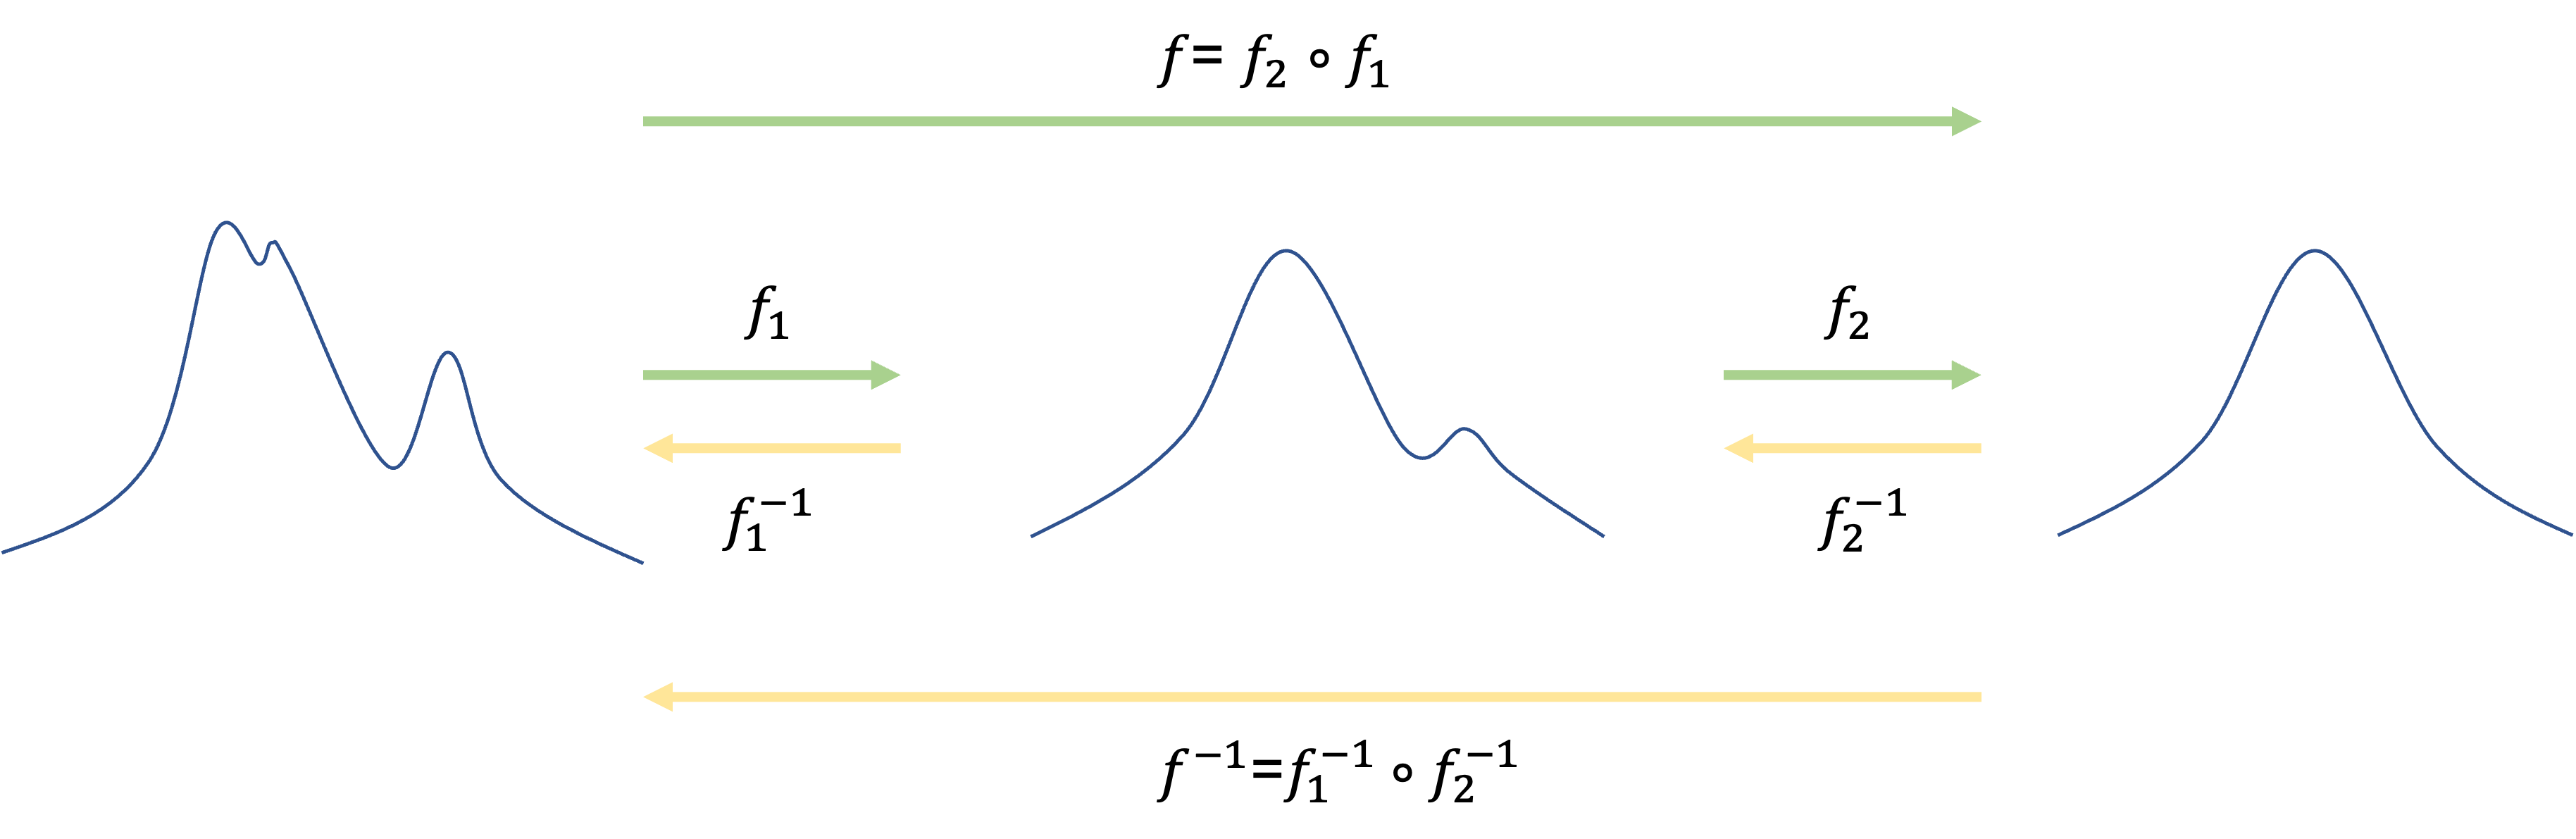
\includegraphics[width=0.8\textwidth]{figures/4/nf-trans.pdf}
    \caption{标准化流原理示意图}
    \label{fig:nf-trans}
\end{figure}

如果变换g能够任意复杂,则可以在对两个分布合理假设下,从任意基分布 $p_{\mathbf{Z}}$生成到任意分布 $p_{\mathbf{Y}}$。该理论经过Bogachev等人证明。\cite{bogachevTriangularTransformationsMeasures2005,medvedevCERTAINPROPERTIESTRIANGULAR2008}


\begin{defn}[双射函数]\label{defn:bio}
	数学中,一个由集合X映射至集合Y的函数,若对每一在Y内的y,存在唯一一个在X内的x与其对应,且对每一在X内的x,存在唯一一个在Y内的y与其对应,则此函数为双射函数。 换句话说,如果其为两集合间的一一对应,则f是双射的。即,同时为单射和满射。
\end{defn}

根据定义\ref{defn:bio},双射函数是可逆函数,但实际情况中构造任意复杂非线性可逆函数(双射)是困难的。人们常说的标准流是指便于计算、求逆和计算雅可比行列式的双射。一种方法是注意可逆函数的组合本身是可逆的,并且其雅可比行列式的行列式具有特定形式。实际上,令 $\mathbf{g}_{1}, \ldots, \mathbf{g}_{N}$是N个双射函数的集合,并且定义 $\mathbf{g}$是这N个双射函数的复合函数,f是它的逆函数,如式\ref{equ:gf}所示。
\begin{quotation}\label{equ:gf}
	\begin{eqnarray}
		\left\{\begin{matrix}
		\mathbf{g} & = & \mathbf{g}_{N} \circ \mathbf{g}_{N-1} \circ \cdots \circ \mathbf{g}_{1}
		\\
		\mathbf{f} & = & \mathbf{f}_{1} \circ \cdots \circ \mathbf{f}_{N-1} \circ \mathbf{f}_{N}
		\end{matrix}\right.
		\end{eqnarray}
\end{quotation}


逆函数f雅可比矩阵的行列式由式\ref{equ:jocob}计算而得。

\begin{equation}\label{equ:jocob}
    \operatorname{det} \operatorname{Df}(\mathbf{y})=\prod_{i=1}^{N} \operatorname{det} \operatorname{D} \mathbf{f}_{i}\left(\mathbf{x}_{i}\right)
\end{equation}

其中 $\operatorname{D}\mathbf{f}_{i}(\mathbf{y})=\frac{\partial \mathbf{f}_{i}}{\partial \mathbf{x}}$是 $\mathbf{f}_{i}$的雅可比矩阵,第i个中间流定义如式\ref{equ:xi},通过复合一系列非线性双射函数来构造出更多复杂函数。
\begin{equation}\label{equ:xi}
	\mathbf{x}_{i}=\mathbf{g}_{i} \circ \cdots \circ \mathbf{g}_{1}(\mathbf{z})=\mathbf{f}_{i+1} \circ \cdots \circ \mathbf{f}_{N}(\mathbf{y}) ,  \mathbf{x}_{N} = \mathbf{y}
\end{equation}

\subsection{概率密度估计和采样} 

标准化流可以用来进行概率密度估计。简单假设只有一个流g,并且g被向量 $\theta$参数化。假设基测度$p_{z}$给定并且被向量$\phi$参数化。给定从复杂分布观测的数据集 $\mathcal{D}=\left\{\mathbf{y}^{(i)}\right\}_{i=1}^{M}$,从而可以基于似然估计参数 $\Theta=(\theta, \phi)$。这个例子中,数据的似然如式\ref{equ:likelihood}所示:
\begin{equation}\label{equ:likelihood}
	\begin{aligned}\log p(\mathcal{D} \mid \Theta) & =\sum_{i=1}^{M} \log p_{\mathbf{Y}}\left(\mathbf{y}^{(i)} \mid \Theta\right) \\& =\sum_{i=1}^{M} \log p_{\mathbf{Z}}\left(\mathbf{f}\left(\mathbf{y}^{(i)} \mid \theta\right) \mid \phi\right)+\log \left|\operatorname{det} \operatorname{Df}\left(\mathbf{y}^{(i)} \mid \theta\right)\right|\end{aligned}
\end{equation}


式\ref{equ:likelihood}中第一行表达式是样本在基测度下的对数似然,第二行表达式,被叫做对数行列式或者体积校正,是用来表示标准化流变换导致的体积变化。在训练中,通过调整流参数 $\theta$和基分布参数$\phi$来最大化对数似然。

评估标准化流建模的分布似然需要计算 f(即标准化方向)和它的对数行列式。在训练中通常需要反复计算似然,因此这些计算的效率尤其重要。然而,从标准化流定义的分布中采样需要评估逆函数g(即生成方向)。因此采样表现表现由生成方向决定。即使流必须是理论上可逆的,逆函数的计算实际上也可能很难。因此,对于概率密度估计,常常是在标准化方向上建模流(即f)。 

\subsection{耦合流}
\begin{figure}[htbp]
    \centering
    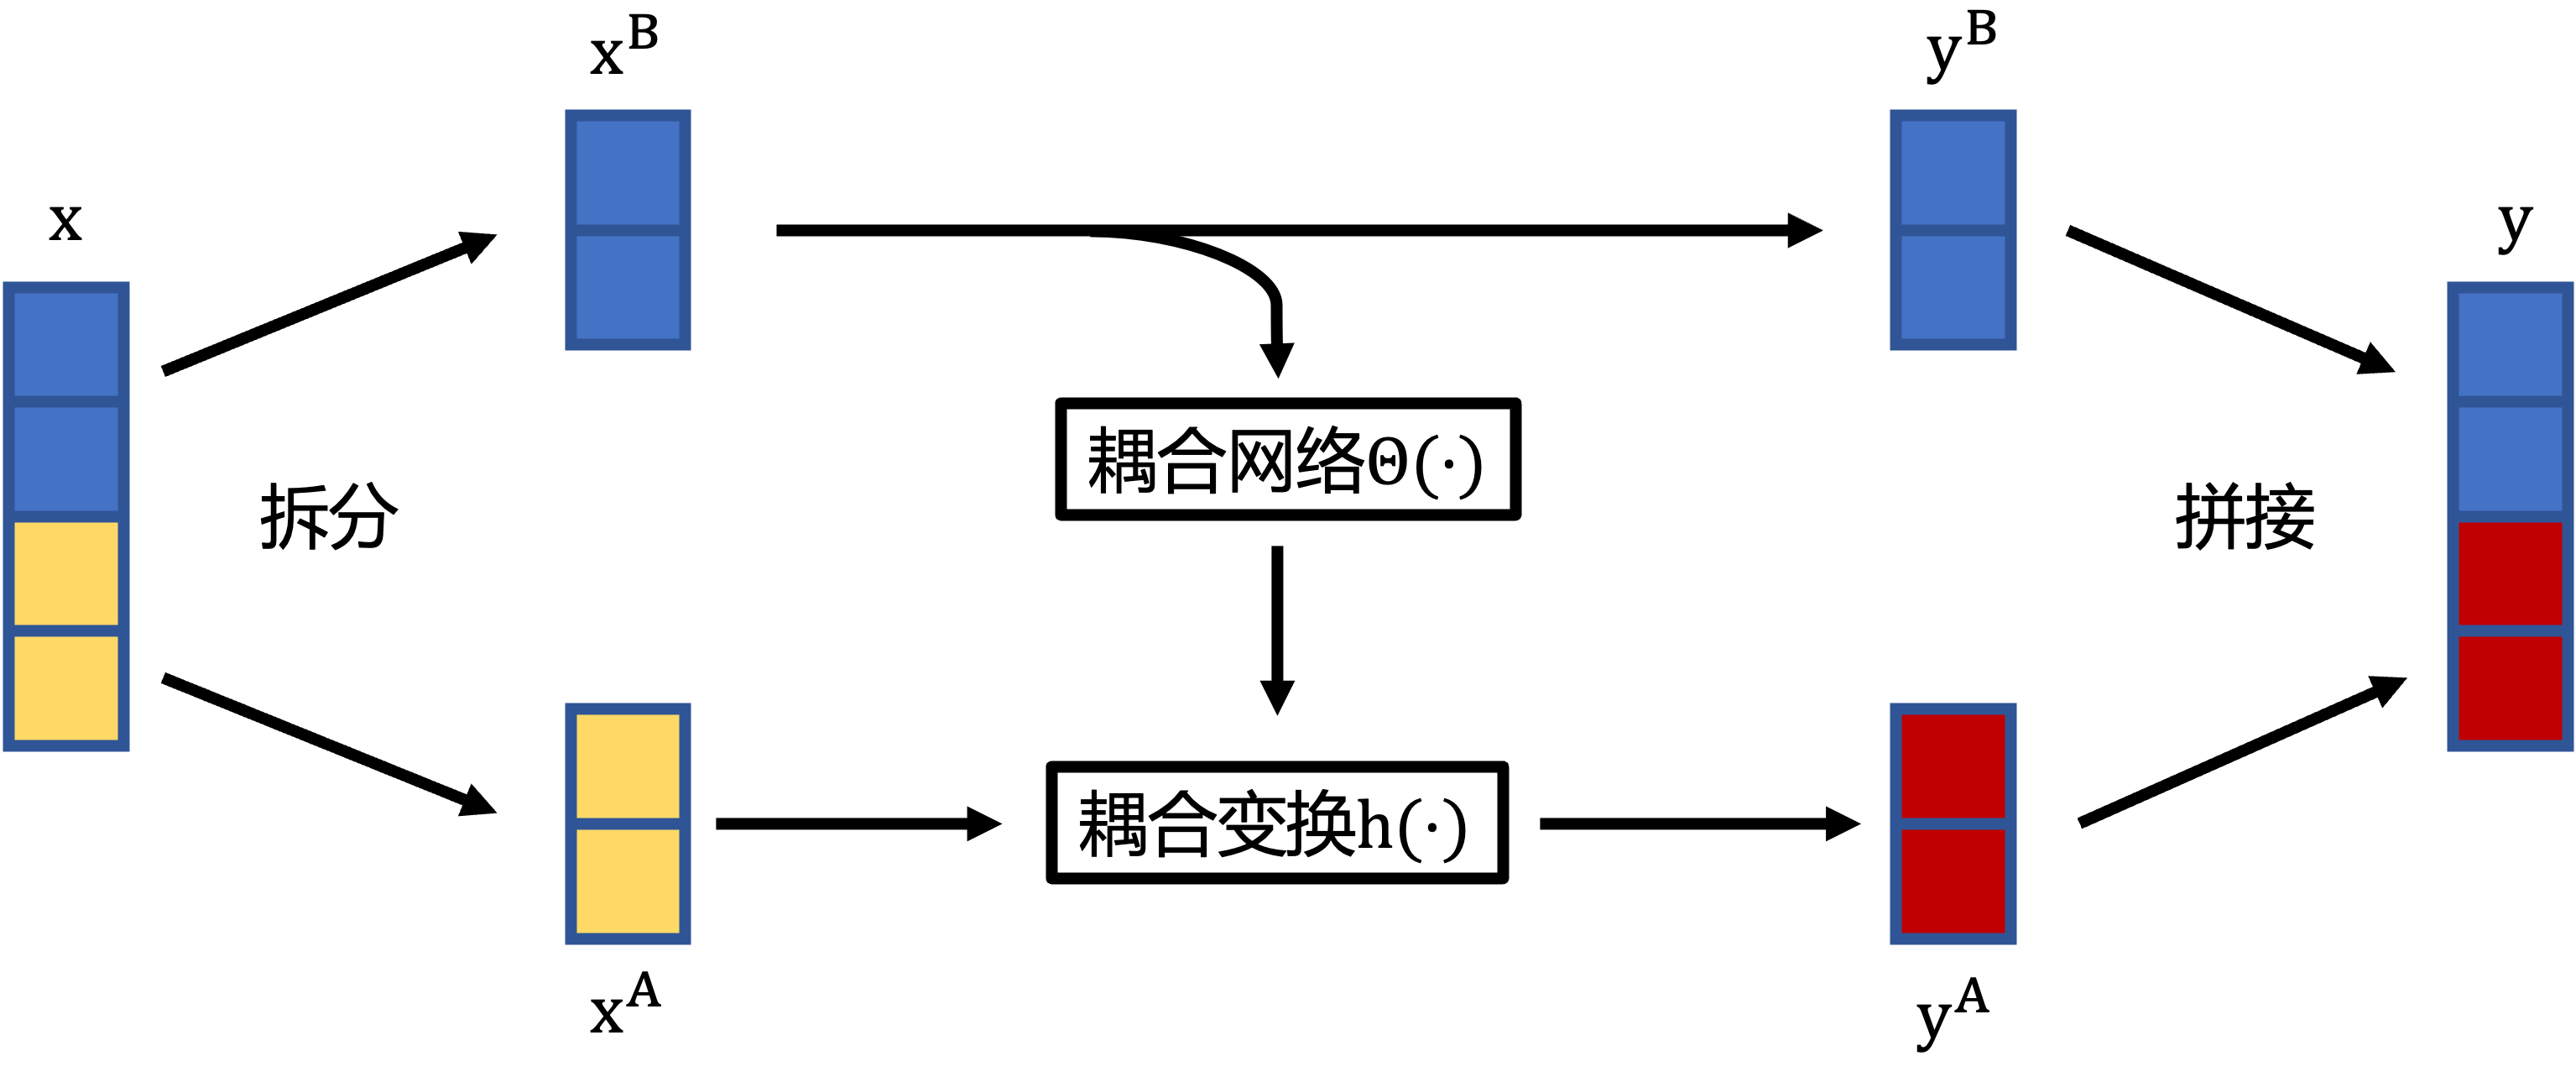
\includegraphics[width=0.75\textwidth]{figures/4/nf-coupling.pdf}
    \caption{耦合流原理示意图}
    \label{fig:nf-coupling}
\end{figure}
为了使标准化流更有计算效率,从而切实可行地来估计概率密度,Dinh等人\cite{dinhNICENonlinearIndependent2015}引入一种耦合的方法为流带来高度表达变换,其原理如图\ref{fig:nf-coupling} 所示。


耦合流将输入 $\mathbf{x} \in \mathbb{R}^{D}$划分为两个子空间 $\left(\mathbf{x}^{A}, \mathbf{x}^{B}\right) \in \mathbb{R}^{d} \times \mathbb{R}^{D-d}$ 并且定义双射函数 $\mathbf{h}(\cdot ; \theta): \mathbb{R}^{d} \rightarrow \mathbb{R}^{d}$,其参数为 $\theta$。定义函数g 如式\ref{equ:coupling-g}所示。
\begin{equation}\label{equ:coupling-g}
    \left\{\begin{matrix}
        \begin{aligned}
        \mathbf{y}^{A} & =\mathbf{h}\left(\mathbf{x}^{A} ; \Theta\left(\mathbf{x}^{B}\right)\right) \\
        \mathbf{y}^{B} & =\mathbf{x}^{B}
        \end{aligned} 
        \end{matrix}\right.
\end{equation}

其中参数 $\theta$定义为只使用 $\mathbf{x}^{B}$作为输入的任一任意函数 $\Theta\left(\mathbf{x}^{B}\right)$。这个函数叫做调节器。双射函数 h 叫做耦合函数,函数g叫做耦合流。一个耦合流是可逆的当且仅当h 是可逆的,其可逆公式如式\ref{equ:converse}所示。

\begin{equation}\label{equ:converse}
    \left\{\begin{matrix}
        \begin{array}{l}\mathbf{x}^{A}=\mathbf{h}^{-1}\left(\mathbf{y}^{A} ; \Theta\left(\mathbf{x}^{B}\right)\right) \\\mathbf{x}^{B}=\mathbf{y}^{B}\end{array}
        \end{matrix}\right.
\end{equation}

g的雅可比矩阵是分块三角矩阵,对角块分别是 $\operatorname{D}\mathbf{h}$和单位阵。因此耦合层雅可比矩阵的行列式就简化为 $\operatorname{D}\mathbf{h}$的行列式,如式\ref{equ:h}所示。

\begin{equation}\label{equ:h}
    \mathbf{h}\left(\mathbf{x}^{A} ; \theta\right)=\left(h_{1}\left(x_{1}^{A} ; \theta_{1}\right), \ldots, h_{d}\left(x_{d}^{A} ; \theta_{d}\right)\right)
\end{equation}


大多数耦合函数是按元素应用到$\mathbf{x}^{A}$,如式。其中每个 $h_{i}\left(\cdot ; \theta_{i}\right): \mathbb{R} \rightarrow \mathbb{R}$是一个标量双射。在这种情况下一个耦合流是一个三角变换(即有一个三角雅可比矩阵)。

耦合流的调节器$\Theta\left(\mathbf{x}^{B}\right)$可以是任意复杂,这是其关键变量。在实际应用中,通常将调节器建模为一个神经网络。

此外,调节器可以是不变的(即完全不依赖 $\mathbf{x}^{B}$),从而实现构建多尺度流。Dinh等人\cite{lelanPerfectDensityModels2021}在生成方向的分布引入了维度。在标准化方向,这个维度每个迭代步骤减半,这样大部分语义信息保留。这减少了转换高维分布的计算成本并且可以捕获某些类型的数据 (例如自然图像) 中固有的多尺度结构。

如何划分x是耦合流的另一个变量,通常在将输入随机排列后进行对半划分。除此之外还有一些常见的结构划分操作,例如,在非体积保持流中的图像的情况下,使用交替像素或通道块的“掩膜”流。

\subsection{仿射耦合函数} 

NICE\cite{dinhNICENonlinearIndependent2015}、RealNVP\cite{dinhDensityEstimationUsing2017}、Glow\cite{kingmaGlowGenerativeFlow2018}使用仿射耦合函数来实现耦合流,其简单、易于计算而且能表示复杂的分布。仿射耦合函数 $h: \mathbb{R} \rightarrow \mathbb{R}$的定义如式\ref{equ:hxtheta}所示。
\begin{equation}\label{equ:hxtheta}
    h(x ; \theta)=\theta_{1} x+\theta_{2}, \quad \theta_{1} \neq 0, \theta_{2} \in \mathbb{R} .
\end{equation}


L2范数利用网络的中间层的特征图提取的特征向量符合多元高斯分布的先验假设。本文采用上述耦合函数构成的标准化流进行概率密度估计,标准化流的输入 $x \in \mathbb{R}^{w \times h \times n_{\text {feat }}}$是尺寸为 $w \times h$有 $n_{feat}$特征的特征图。在这些块中。在随机选择保持固定的排列之后,输入 $x$的通道沿着通道均匀地划分为部分 $\mathbf{x}^{A}$和 $\mathbf{x}^{B}$。这些部分中的每一个作为静态条件都与位置编码c拼接。

为了充分利用所有信息,一般对两部分交替进行仿射变换。本文通过为每个部分建立 $s_{i}$和 $t_{i}$的子网络来实现仿射变换,如式\ref{equ:y2y1}所示。

\begin{equation}\label{equ:y2y1}
    \left\{\begin{matrix}
        \begin{array}{c}y_{2}=x_{2} \odot e^{s_{1}\left(\left[x_{1}, c\right]\right)}+t_{1}\left(\left[x_{1}, c\right]\right) \\y_{1}=x_{1} \odot e^{s_{2}\left(\left[x_{2}, c\right]\right)}+t_{2}\left(\left[x_{2}, c\right]\right)\end{array}
        \end{matrix}\right.
\end{equation}

其中 $\odot$是元素的乘积, $\left[ ·,·\right]$表示沿通道拼接。一个耦合块的输出是沿着通道对$y_{1}$和$y_{2}$的拼接,输入和输出的维数保持一致。

\subsection{位置编码} 

在仿射耦合函数应用标准化流的基础上,本文还参考CFLOW-AD\cite{gudovskiyCFLOWADRealTimeUnsupervised2022}的做法引入条件变量,用位置编码 $\boldsymbol{c}_{pos} \in \mathbb{R}^{D}, pos \in\left\{w \times h\right\}$拼接解码器耦合层的中间变量从而扩展了无条件流框架。

位置编码的实现方法参考Transformer\cite{vaswaniAttentionAllYou2017}中提出的方法,使用如式\ref{equ:positionencoder}所示的不同频率正弦和余弦函数。

\begin{equation}\label{equ:positionencoder}
    \left\{\begin{matrix}
    \begin{aligned}P E_{(p o s, 2 d)} & =\sin \left(\frac{p o s}{10000^{\frac{2 d}{n_{\text {feat }}}}}  \right) \\P E_{(p o s, 2 d+1)} & =\cos \left(\frac{p o s}{10000^{\frac{2 d}{n_{\text {feat }}}}}  \right)\end{aligned}
\end{matrix}\right.
\end{equation}

其中 pos是位置,d是维度。每个位置编码的维度都对应一个正弦。考虑对每一个固定的偏移k, $P E_{p o s+k}$能够表示为 $P E_{p o s}$的线性函数,CFLOW-AD假设该函数对模型按相对位置学习是有益的。

此外,在Transformer中实验的表明,使用通过学习获得的位置嵌入和通过正弦获得嵌入的效果相差不大,但选择正弦版本可以在推广模型到对其它长度序列进行位置编码时减少训练量。


\begin{figure}[htbp]
    \centering
    \includegraphics[width=0.9\textwidth]{figures/4/teacher.pdf}
    \caption{教师网络结构}
    \label{fig:nf-teacher}
\end{figure}

教师网络结构如图\ref{fig:nf-teacher}所示。使用变量公式的变化z作为最终输出如式\ref{equ:px}所示。

\begin{equation}\label{equ:px}
    p_{X}(x)=p_{Z}(z)\left|\operatorname{det} \frac{\partial z}{\partial x}\right|
\end{equation}

生成模型的目标就是对目标数据的分布进行建模,其通常利用极大似然估计或最小化某些差异来评估。教师网络以 $p_{Z}$为正态分布 $\mathcal{N}(0, I)$ ,通过优化在像素位置 $(i,j)$全部前景像素的均值来最小化负对数似然,教师网络损失如式\ref{equ:teacherloss}所示。本文不直接以教师网络输出计算异常分数,而是将训练教师网络作为训练学生网络的前置任务。

\begin{equation}\label{equ:teacherloss}
    \mathcal{L}_{i j}^{t}=-\log p_{X}\left(x_{i j}\right)=\frac{\left\|z_{i j}\right\|_{2}^{2}}{2}-\log \left|\operatorname{det} \frac{\partial z_{i j}}{\partial x_{i j}}\right|
\end{equation}


\section{学生网络}
本文采用异构的教师学生网络组合,学生网络是一个包含残差块的简单全卷积网络,而没有采用教师网络的可逆变换。学生网络的每个残差块由3×3卷积层的两个序列组成,利用批归一化\cite{ioffeBatchNormalizationAccelerating2015}和leaky ReLU激活。学生网络在残差块前后各设一层卷积来保证特征维度与教师网络一致。

在网络输入阶段,本文将深度图像和其HOG特征在输入学生网络前先拼接,然后再经过两层专门为深度特征混合图的卷积层来提取深度图的特征,最后再和RGB特征一起通过卷积层融合然后输入残差块。学生网络结构如图\ref{fig:student}所示
\begin{figure}[htbp]
    \centering
    \includegraphics[width=0.9\textwidth]{figures/4/student.pdf}
    \caption{学生网络结构}
    \label{fig:student}
\end{figure}

此外,位置编码c在输入学生网络前进行了拼接,其输出维度与教师匹配从而实现逐像素的距离计算。学生网络的目标是最小化在训练样本 $x \in X$的学生输出 $f_{s}(x)$和教师输出 $f_{t}(x)$之间的  $\ell_{2} \text {-distance }$的平方。给定训练集 $X$,在像素位置 $(i,j)$的输出如式\ref{equ:studentloss}所示。

\begin{equation}\label{equ:studentloss}
    \mathcal{L}_{i j}^{s}=\left\|f_{s}(x)_{i j}-f_{t}(x)_{i j}\right\|_{2}^{2}   
\end{equation}


在所有(前景)像素上平均 $\mathcal{L}_{i j}^{s}$即可得到最后的损失 $\mathcal{L}^{s}$,其也被用于计算排除背景像素的图像级异常得分,本文通过计算像素上的最大值或平均值来聚合一个样本的像素距离。
\section{实验设计及结果分析}
\subsection{数据集}
本文使用第二章搭建的实验平台,对实验室的塑料工件进行拍摄,采集用于训练和验证的数据。首先是采集正常样本,实验平台按照设定从多个角度全自动采集出192组图像,每组图像均由RGB图像和深度图像组成,其中部分正常样本组如图\ref{fig:normal-smaple}所示。
\begin{figure}[htbp]
    \centering
    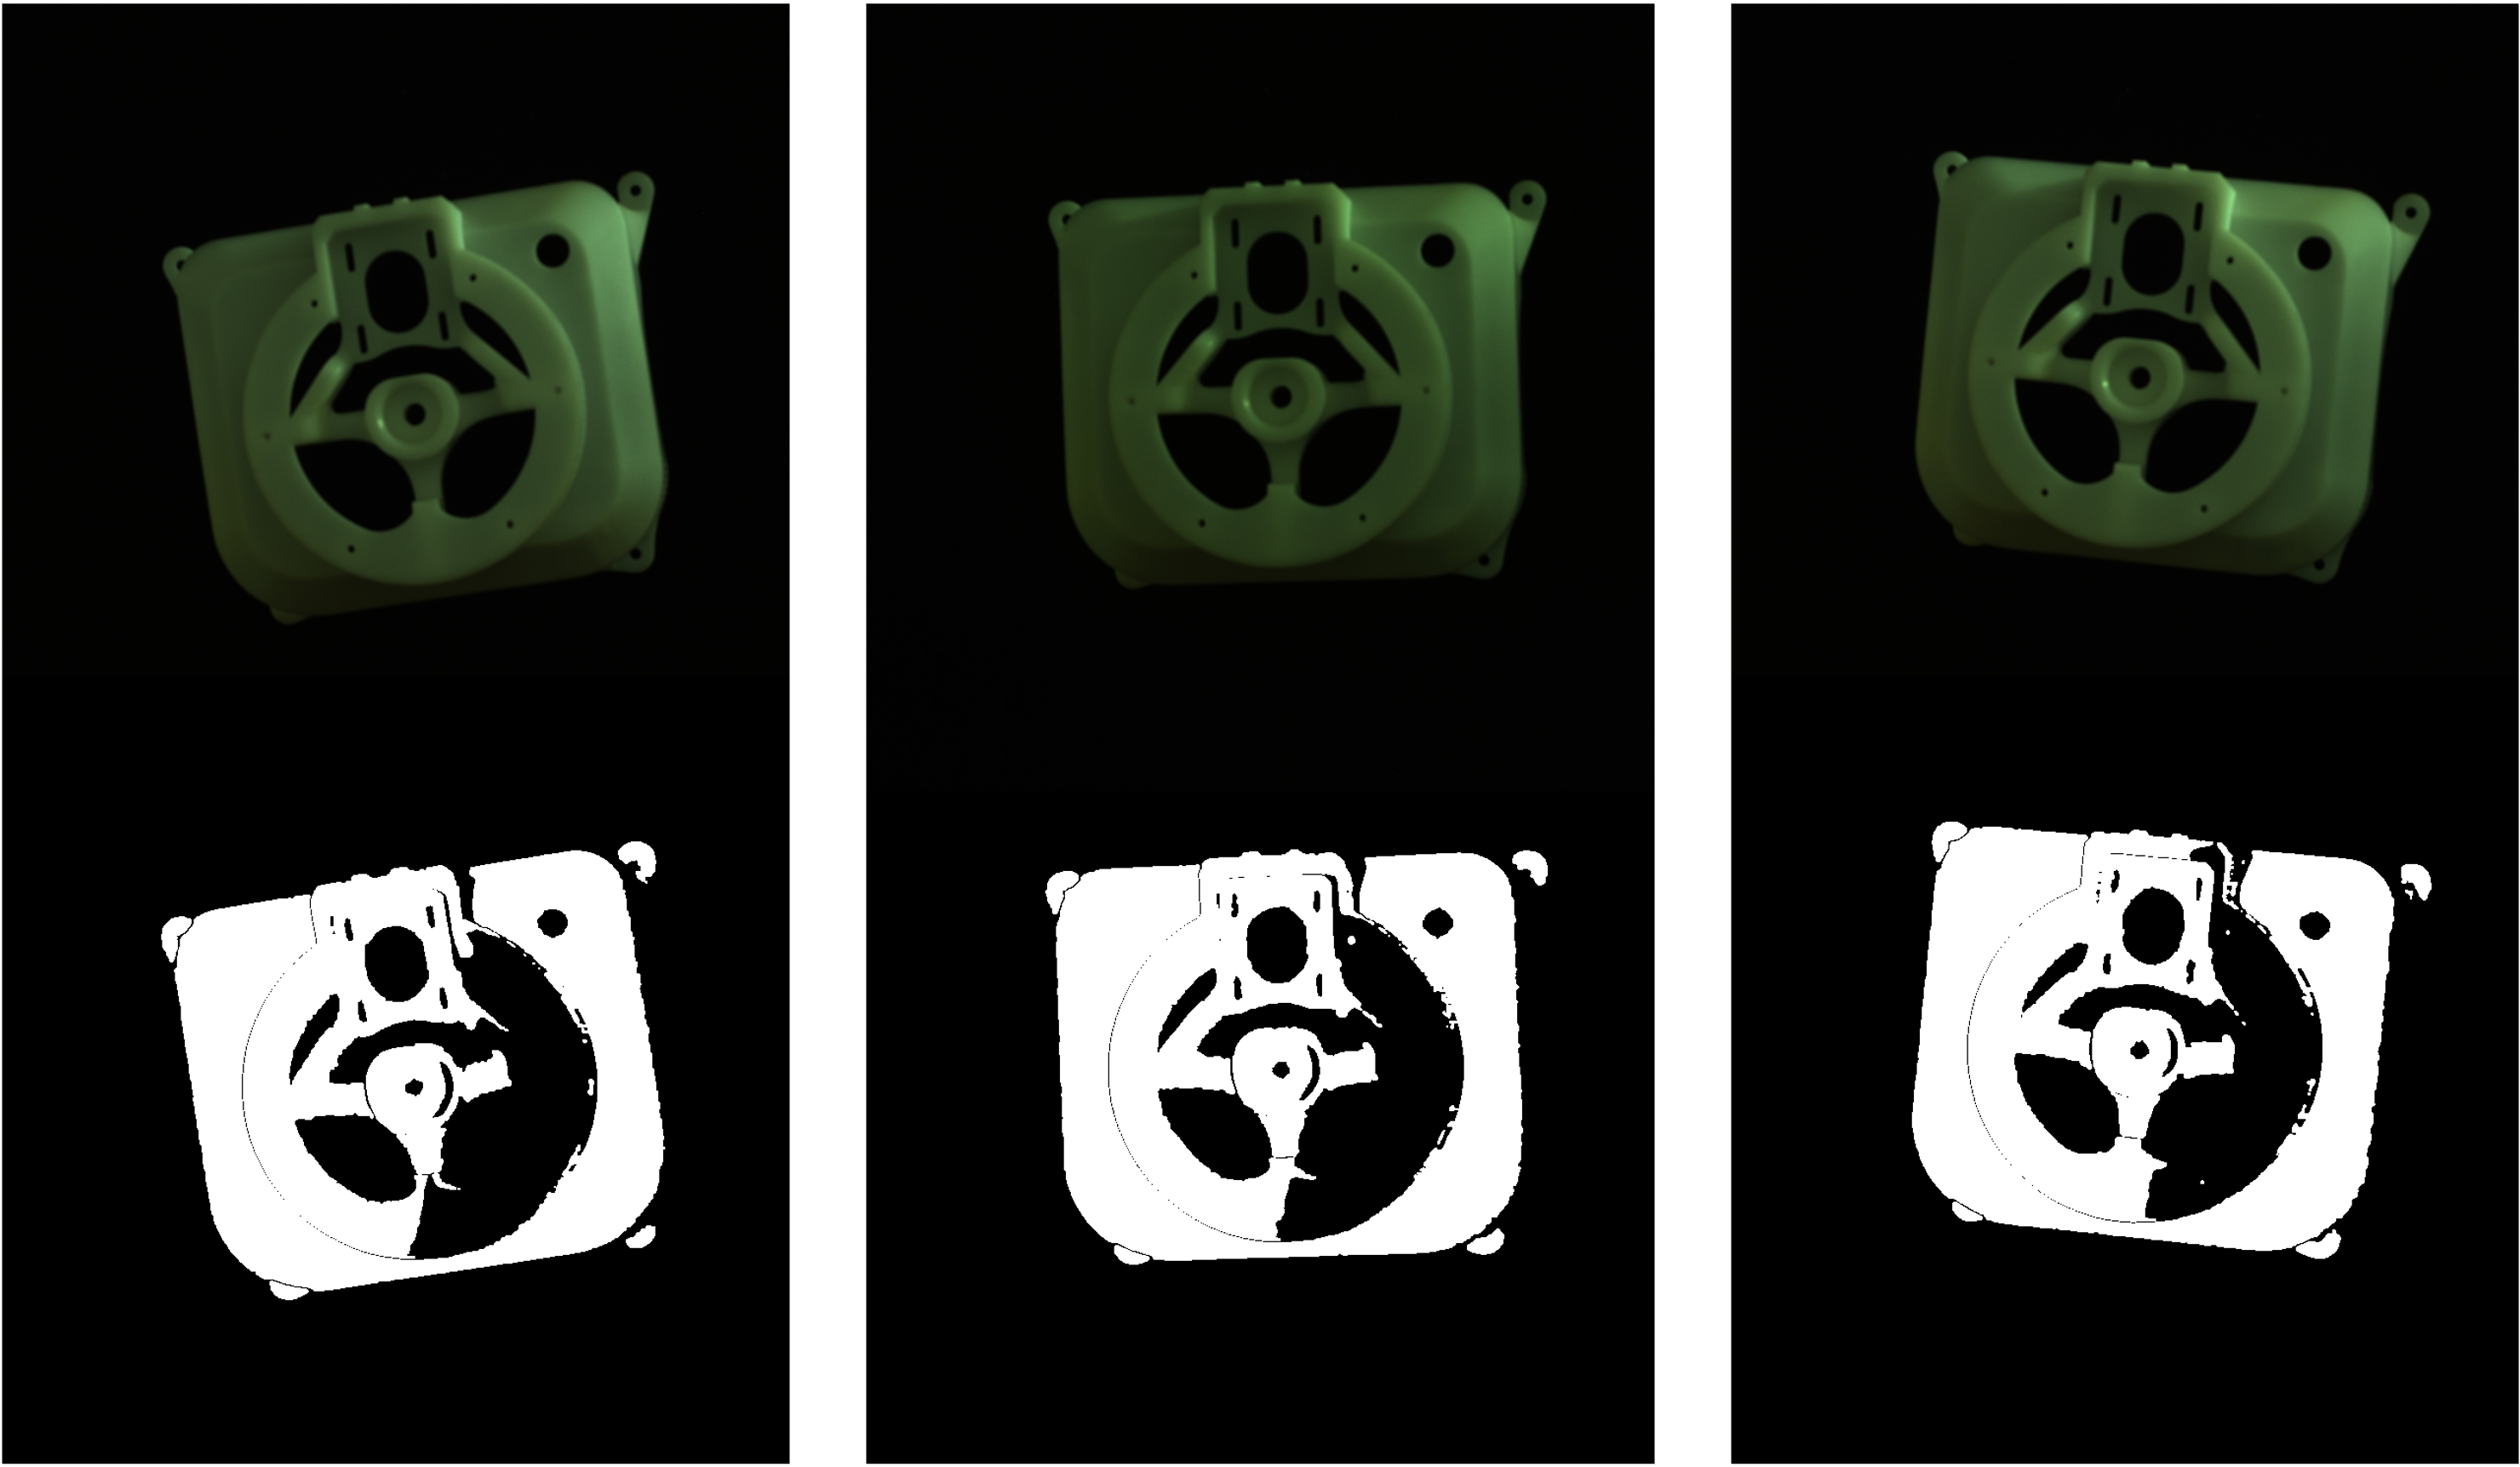
\includegraphics[width=0.75\textwidth]{figures/4/normal-smaple.png}
    \caption{正常样本}
    \label{fig:normal-smaple}
\end{figure}

为了检验本文的多模态缺陷算法的性能,本文又通过手工制造了三类五种缺陷模拟可能存在的缺陷类型,这些缺陷样本总共有96组。其中第一类缺陷为结构变型缺陷,包括横向和纵向变型,如图\ref{fig:bad-1}所示,其中左图为横向变型,右图为纵向变型。
\begin{figure}[htbp]
    \centering
    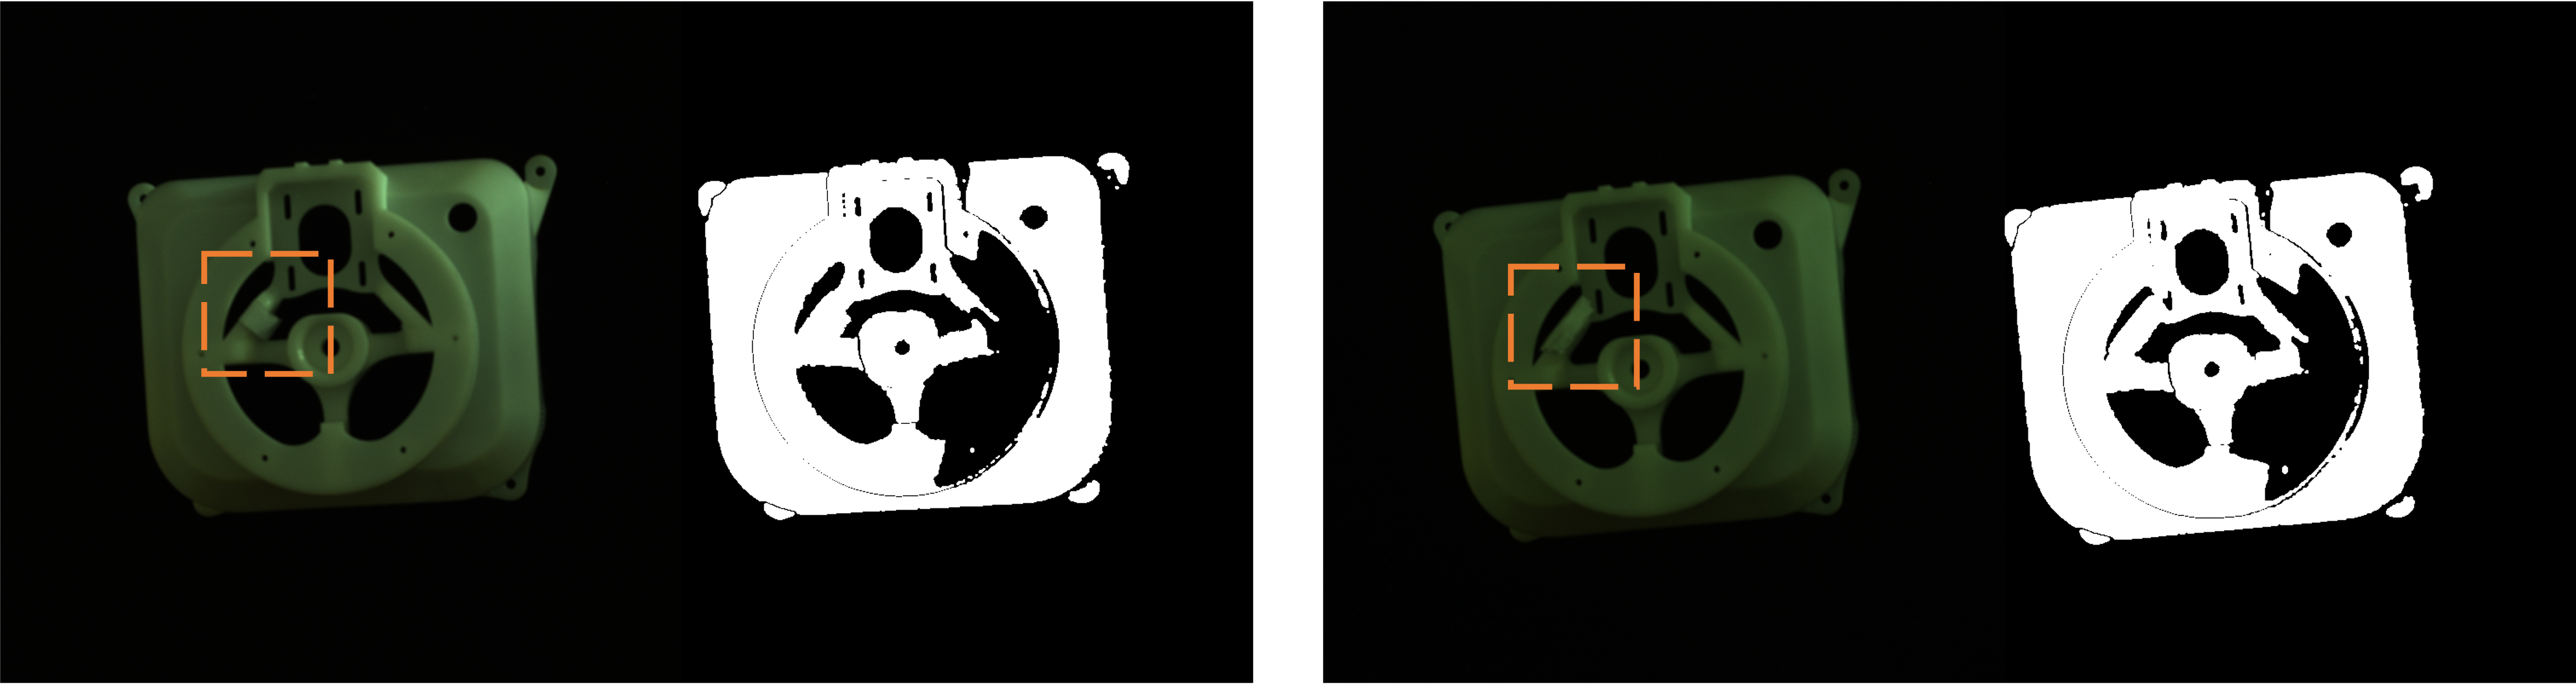
\includegraphics[width=1\textwidth]{figures/4/bad-1.png}
    \caption{结构变型缺陷}
    \label{fig:bad-1}
\end{figure}

第二类缺陷为空洞填充缺陷,如图\ref{fig:bad-2}所示,其中左图展示的整个空洞完全填充的缺陷,右图展示的是空洞单侧填充的缺陷。
\begin{figure}[htbp]
    \centering
    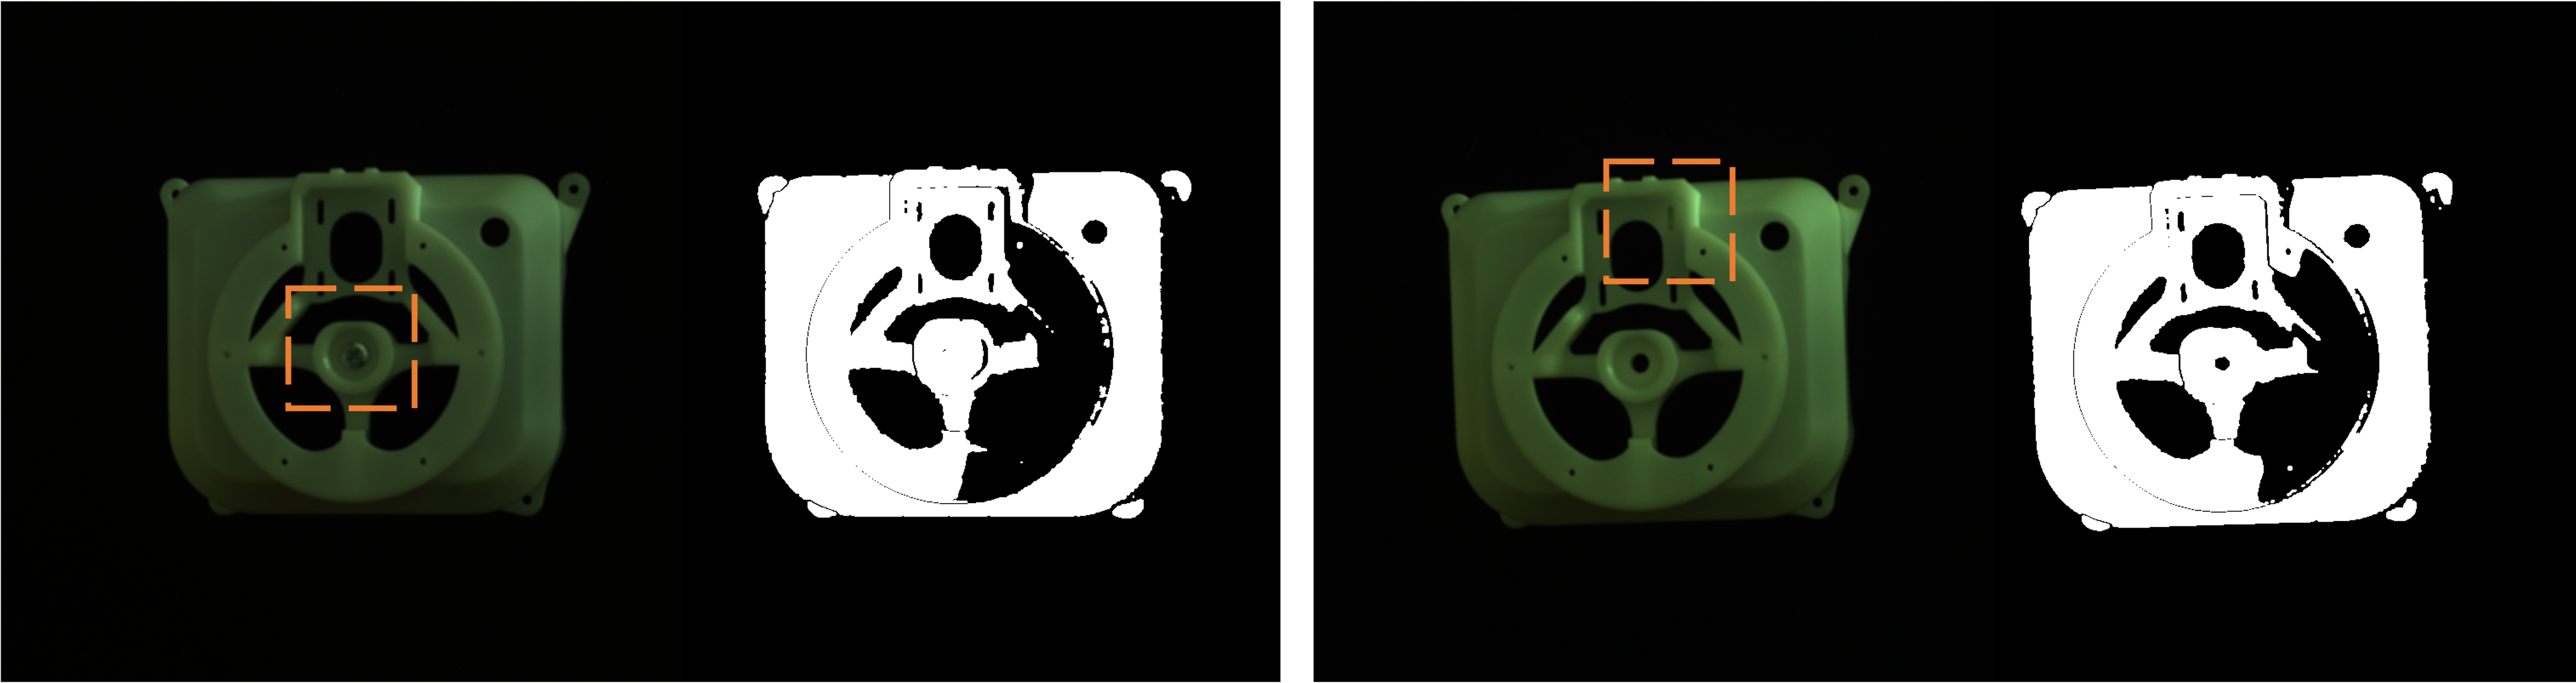
\includegraphics[width=1\textwidth]{figures/4/bad-2.png}
    \caption{空洞填充缺陷}
    \label{fig:bad-2}
\end{figure}

第三类缺陷为划痕和杂色缺陷,如图\ref{fig:bad-3}中的红色浅划痕。
\begin{figure}[htbp]
    \centering
    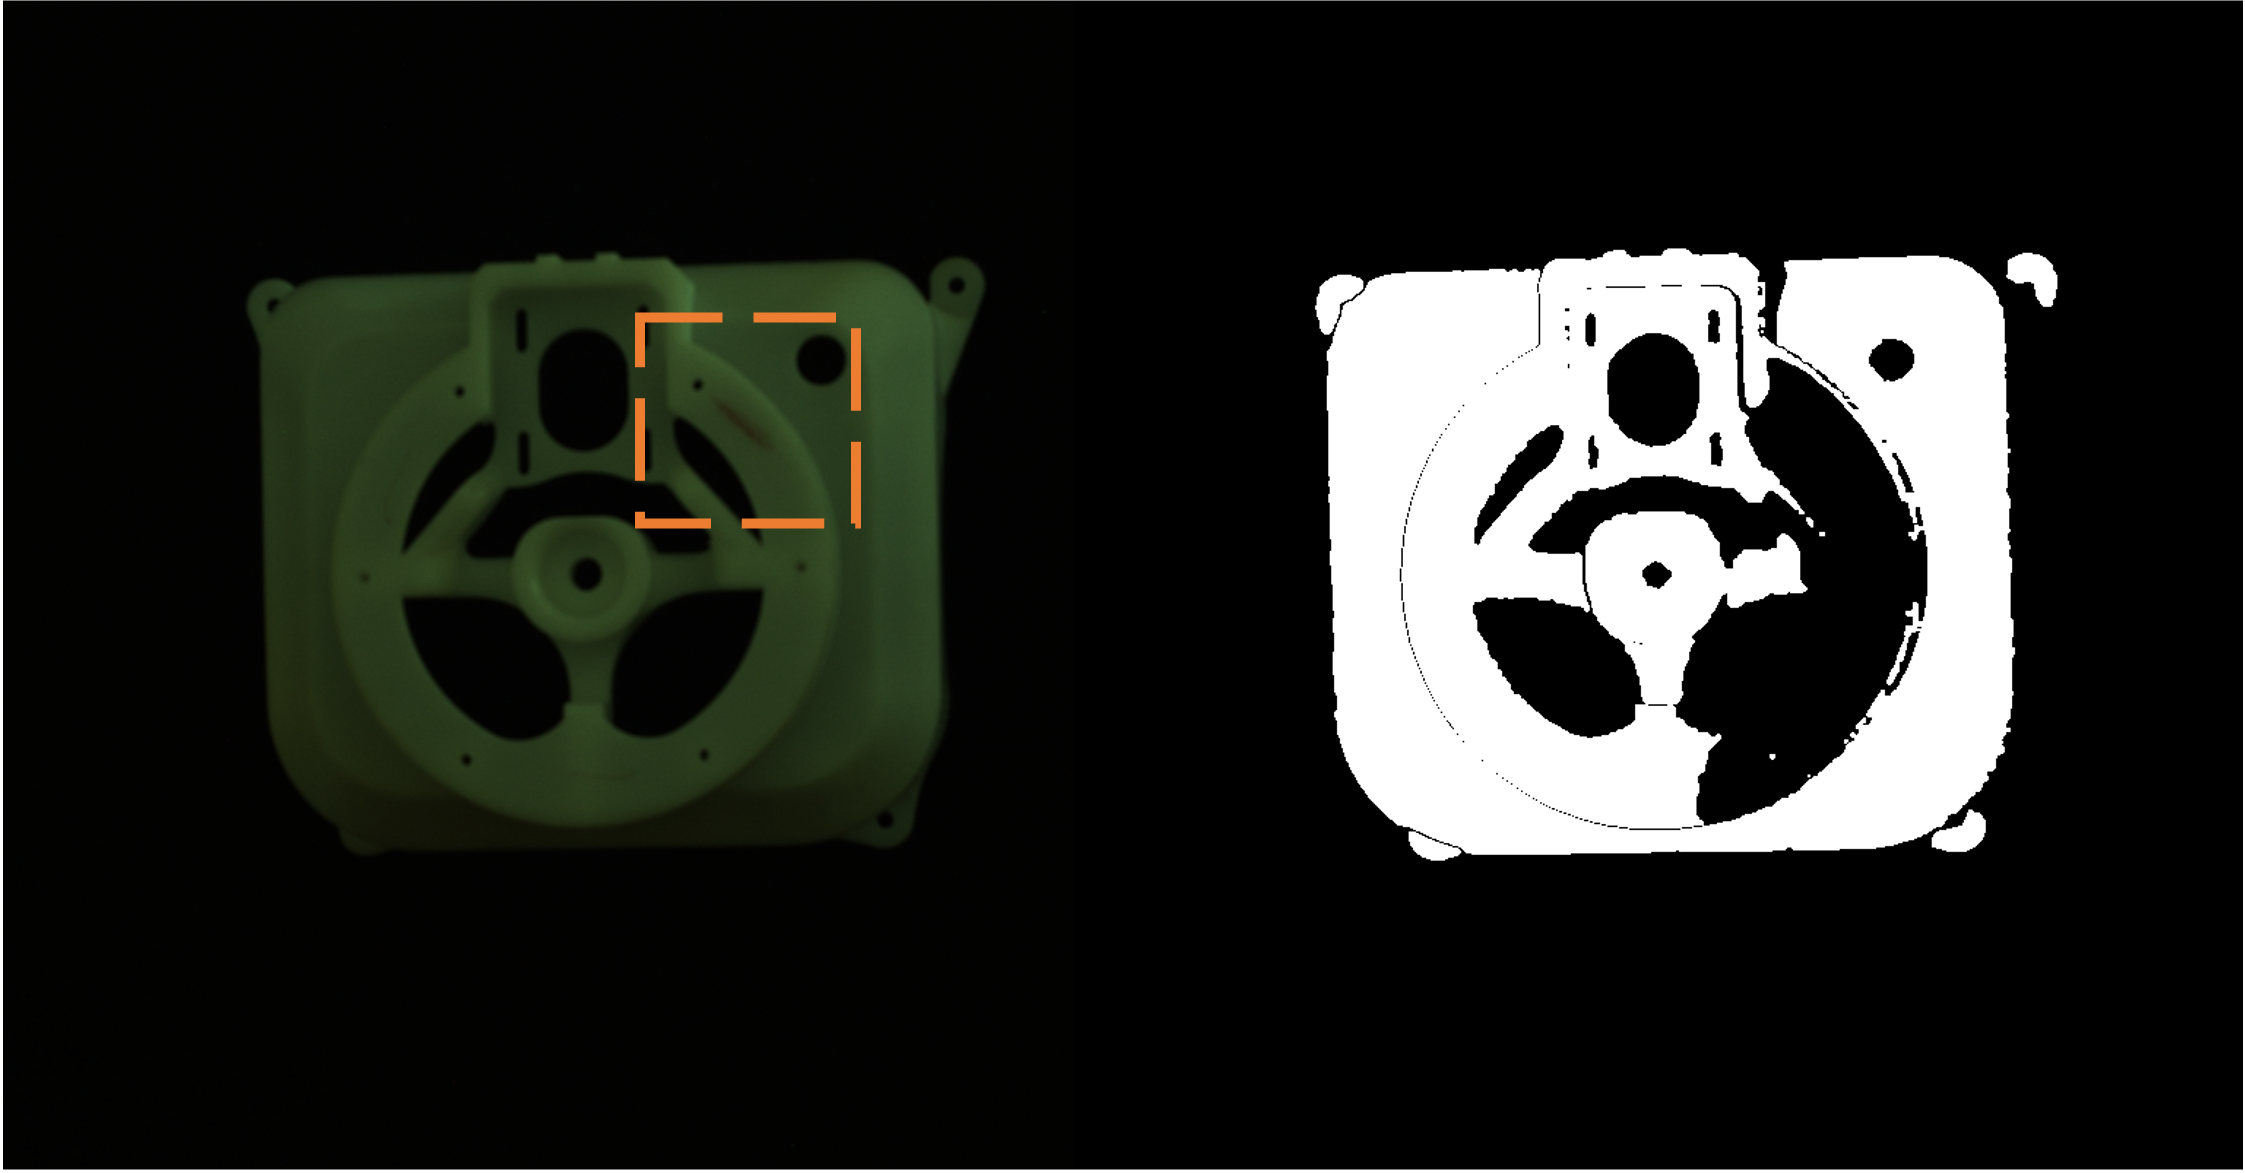
\includegraphics[width=0.6\textwidth]{figures/4/bad-3.png}
    \caption{划痕和杂色缺陷}
    \label{fig:bad-3}
\end{figure}

本文将上述正常样本和缺陷样本组合建立用于模型训练和验证的数据集,数据集的结构表\ref{tab:4-dataset}所示。
\begin{table}[htbp]
    \centering
    \caption{数据集} \label{tab:4-dataset}
    \begin{tabular*}{0.75\textwidth}{@{\extracolsep{\fill}}ccc}
    \toprule
    %   数据集&正常样本&变型缺陷&填充缺陷&划痕杂色缺陷&混合缺陷\\
    % \midrule
    %   训练集&160&-&-	&-&- \\
    %   测试集	&32	&32 &32	&16&16			 \\
      &正常样本&缺陷样本\\
      \midrule
        训练集&160&-\\
        测试集	&32&96\\
      
    \bottomrule
    \end{tabular*}
\end{table}
\subsection{实验设计}
根据对输入深度图像值处理的方式不同,本文设计了四个对比实验,如表\ref{tab:4-experiment-desgin}所示。其中AST是原始模型,通过对深度图像原始像素进行块混合下采样的方式来使深度图像与预训练的RGB特征图维数匹配;H-AST是在AST的基础上引入HOG对深度图像进行特征提取后再在维度上进行拼接;F-AST是对输入学生网络的深度图像先进行两层卷积后再与RGB特征图拼接然后输入残差块;HF-AST则是结合HOG和学生网络卷积层对深度图像特征提取。其中HF-AST是本文提出的新方法,H-AST和F-AST是对该方法的一个消融实验。
\begin{table}[htbp]
    \centering
    \caption{实验设计} \label{tab:4-experiment-desgin}
    \begin{tabular*}{0.6\textwidth}{@{\extracolsep{\fill}}cc}
    \toprule
      缺陷检测算法&深度图处理方式\\
      \midrule
        AST&像素值混合\\
        H-AST	&HOG\\
        F-AST&学生网络卷积\\
        HF-AST	&HOG+学生网络卷积\\
      
    \bottomrule
    \end{tabular*}
\end{table}

\subsection{实验结果分析}
\begin{figure}[htbp]
    \centering
    \begin{subfigure}
        \centering
        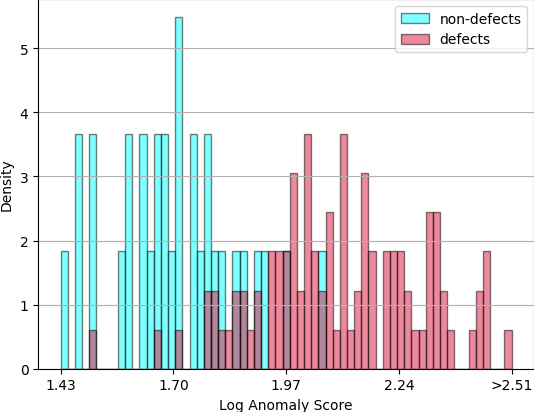
\includegraphics[width=.4\linewidth]{figures/4/hist/ori_experiment/plastics_mean.png}  
      \end{subfigure}
      \begin{subfigure}
        \centering
        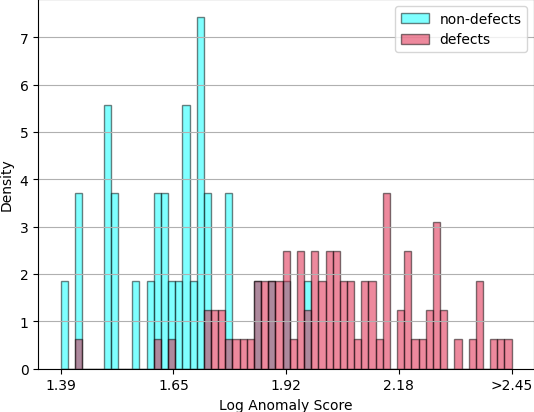
\includegraphics[width=.4\linewidth]{figures/4/hist/hog_experiment/plastics_mean.png} 
      \end{subfigure}
      \begin{subfigure}
        \centering
        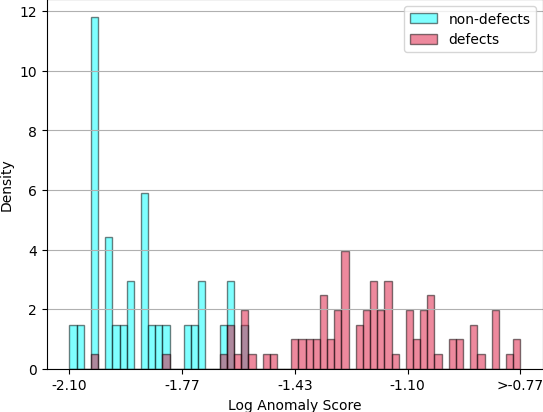
\includegraphics[width=.4\linewidth]{figures/4/hist/mix_experiment/plastics_mean.png} 
      \end{subfigure}
      \begin{subfigure}
        \centering
        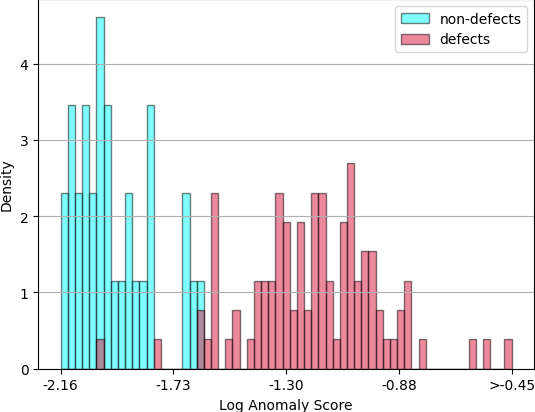
\includegraphics[width=.4\linewidth]{figures/4/hist/mixhog_experiment/plastics_mean.png} 
      \end{subfigure}
    \caption{平均直方图}
    \label{fig:hist_mean}
\end{figure}
按照实验设计,本文进行多次实验,每次实验所有方法除对深度图像处理方法有所差异外,其余各项参数均保持一致。针对本文的多模态缺陷检测,本文分别采用了平均距离和最大距离来计算图像级异常得分,实验结果如下列图像所示。其中直方图用于统计测试集异常得分情况,蓝色柱表示测试集中正常样本的异常得分分布,红色柱则表示缺陷样本。AUROC图则是衡量缺陷检测算法性能的指标。在每组图片中,左上为AST,右上为H-AST,左下为F-AST,右下为HF-AST。

组图\ref{fig:hist_mean}是根据平均距离计算测试集对数异常得分的统计直方图。从组图中可以看到表示正常样本的蓝色柱和表示缺陷样本的红色柱呈现两个不同分布,但同时两者有所相交。

\begin{figure}[htbp]
    \centering
    \begin{subfigure}
        \centering
        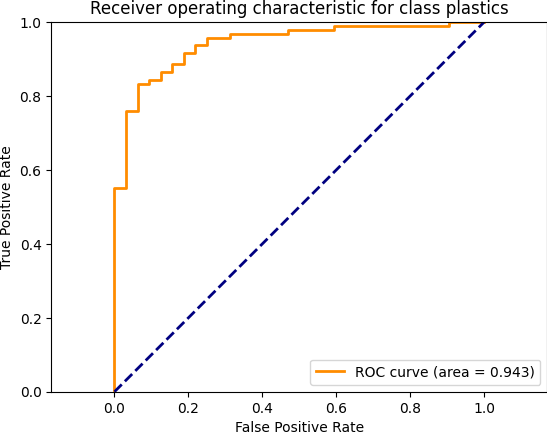
\includegraphics[width=.4\linewidth]{figures/4/auroc/ori_experiment/plastics_mean.png}  
        \end{subfigure}
        \begin{subfigure}
        \centering
        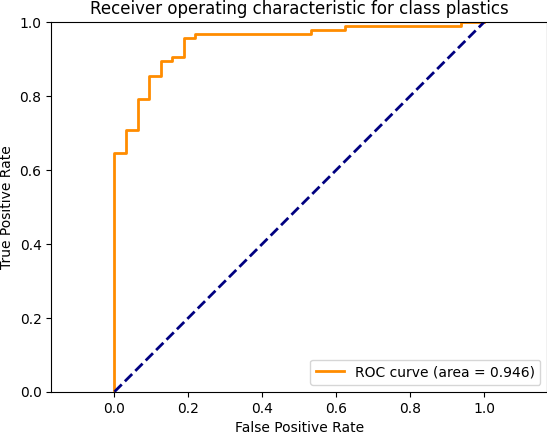
\includegraphics[width=.4\linewidth]{figures/4/auroc/hog_experiment/plastics_mean.png} 
        \end{subfigure}
        \begin{subfigure}
        \centering
        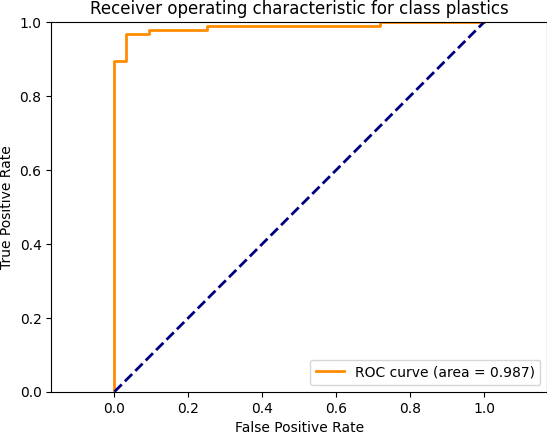
\includegraphics[width=.4\linewidth]{figures/4/auroc/mix_experiment/plastics_mean.png} 
        \end{subfigure}
        \begin{subfigure}
        \centering
        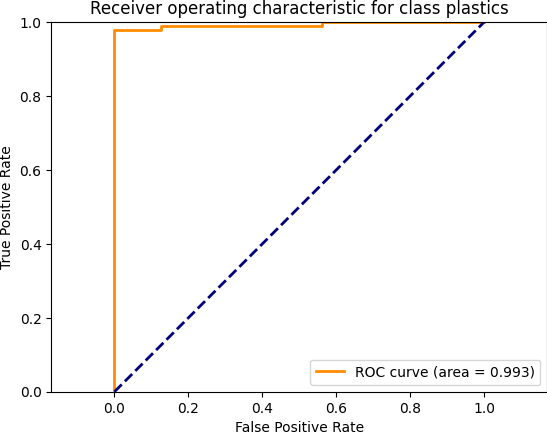
\includegraphics[width=.4\linewidth]{figures/4/auroc/mixhog_experiment/plastics_mean.png} 
        \end{subfigure}
    \caption{平均AUROC}
    \label{fig:auroc_mean}
    \end{figure}
组图\ref{fig:auroc_mean}是根据平均距离计算的AUROC。从图中可以看出本文实验的所有方法采用平均距离衡量均能取得不错的表现,HF-AST方法在平均距离计算异常得分下实现99.3\%的AUROC,超过其它方法。此外,H-AST和AST以及HF-AST和F-AST的两组实验对比说明加入HOG能够对算法有小幅提升;F-AST和AST以及HF-AST和H-AST的两组实验对比说明使用在学生网络加入深度图像卷积层对缺陷检测性能提升明显。


\begin{figure}[htbp]
\centering
\begin{subfigure}
    \centering
    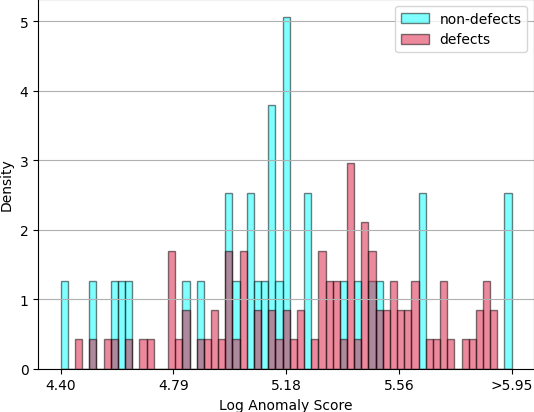
\includegraphics[width=.4\linewidth]{figures/4/hist/ori_experiment/plastics_max.png}  
    \end{subfigure}
    \begin{subfigure}
    \centering
    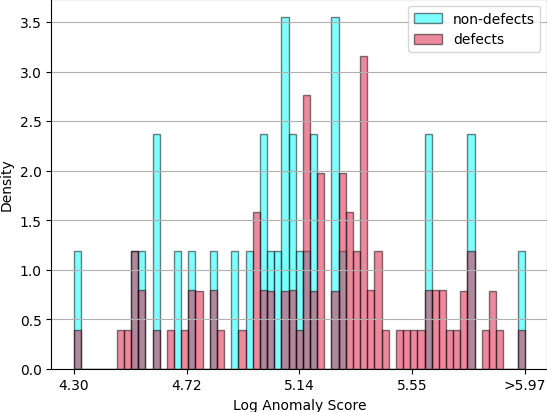
\includegraphics[width=.4\linewidth]{figures/4/hist/hog_experiment/plastics_max.png} 
    \end{subfigure}
    \begin{subfigure}
    \centering
    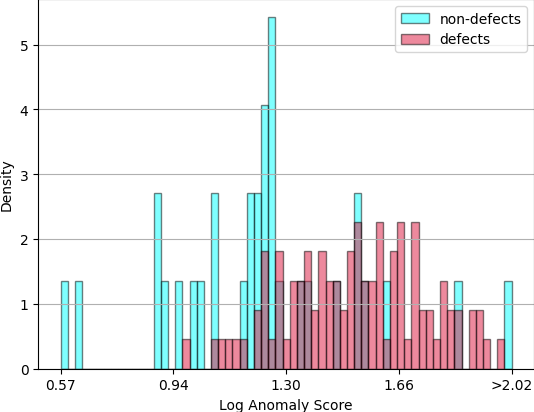
\includegraphics[width=.4\linewidth]{figures/4/hist/mix_experiment/plastics_max.png} 
    \end{subfigure}
    \begin{subfigure}
    \centering
    \includegraphics[width=.4\linewidth]{figures/4/hist/mixhog_experiment/plastics_max.png} 
    \end{subfigure}
\caption{最大直方图}
\label{fig:hist_max}
\end{figure}

\begin{figure}[htbp]
    \centering
    \begin{subfigure}
        \centering
        \includegraphics[width=.4\linewidth]{figures/4/auroc/ori_experiment/plastics_max.png}  
        \end{subfigure}
        \begin{subfigure}
        \centering
        \includegraphics[width=.4\linewidth]{figures/4/auroc/hog_experiment/plastics_max.png} 
        \end{subfigure}
        \begin{subfigure}
        \centering
        \includegraphics[width=.4\linewidth]{figures/4/auroc/mix_experiment/plastics_max.png} 
        \end{subfigure}
        \begin{subfigure}
        \centering
        \includegraphics[width=.4\linewidth]{figures/4/auroc/mixhog_experiment/plastics_max.png} 
        \end{subfigure}
    \caption{最大AUROC}
    \label{fig:auroc_max}
    \end{figure}
组图\ref{fig:hist_max}是根据最大距离计算测试集对数异常得分的统计直方图。从组图中可以看到未引入学生网络深度图像卷积层的原模型的正常样本和缺陷样本分布相近,影响是否有缺陷分类的准确性。


组图\ref{fig:auroc_max}是根据最大距离计算的AUROC。从图中可以看出本文实验的所有方法相较于用平均距离衡量的性能方差要大,HF-AST方法在最大距离计算异常得分下实现85.4\%的AUROC,远超过其它方法。此外,H-AST和AST以及HF-AST和F-AST的两组实验对比说明在引入学生网络深度图像卷积下,加入HOG能够对算法性能提升更为有效;F-AST和AST以及HF-AST和H-AST的两组实验对比说明使用在学生网络加入深度图像卷积层对缺陷检测性能提升显著。

汇总上述实验结果为表\ref{tab:plastics-experiment} ,该表展现了本文提出的改进异构教师学生网络在本文的塑料件上性能提升明显。
\begin{table}[htbp]
    \centering
    \caption{塑料件数据集实验结果} \label{tab:plastics-experiment}
    \begin{tabular*}{0.8\textwidth}{@{\extracolsep{\fill}}ccccc}
    \toprule
      &AST&H-AST&F-AST&HF-AST\\
      \midrule
      mean AUROC&0.943&0.946&0.987&0.993\\
      max AUROC&0.626&0.636&0.798&0.854\\
    \bottomrule
    \end{tabular*}
\end{table}

最后,本文分别应用原始AST模型和本文提出改进的HF-AST模型对空洞填充和结构变型缺陷样本进行缺陷检测并生成热力图。其中组图\ref{fig:featmap-1}是空洞填充缺陷,组图\ref{fig:featmap-2}是结构变型缺陷。组图的第一行分别是输入的RGB图像和深度图像,虚线框包围的是热力图,热力图中颜色越黄则表示该处异常得分越高。

\begin{figure}[htbp]
    \centering
    \includegraphics[width=0.6\textwidth]{figures/4/featmap-1.png}
    \caption{空洞填充热力图}
    \label{fig:featmap-1}
\end{figure}

\begin{figure}[htbp]
    \centering
    \includegraphics[width=0.6\textwidth]{figures/4/featmap-2.png}
    \caption{结构变型热力图}
    \label{fig:featmap-2}
\end{figure}


\section{本章小节}
本章首先对采集的多模态数据——RGB和深度图像进行预处理,然后分别通过预训练的EfficientNet网络对RGB图像提取特征图和迁移HOG特征描述子到深度图像来提取深度特征,接着分别介绍了本章缺陷检测骨干网络中的标准化流的教师网络和本文改进深度特征融合的学生网络原理。在本章最后的实验阶段,对比了引入HOG提取深度特征和改进学生网络对缺陷算法性能提升,证明了本文提出方法的有效性。

















% \begin{algorithm}
%     \caption{Depth Image Normalization 深度图像归一化}
%     \begin{algorithmic}[1]
%     \Function{NormalizeDepthImage}{$depth\_image$}
%         \State $depth\_image\_float \gets \Call{ConvertToFloat}{depth\_image}$  \Comment{转换为浮点数格式}
%         \State $depth\_image\_float \gets \Call{ReplaceInvalidValues}{depth\_image\_float}$  \Comment{去除无效值}
%         \State $min\_depth, max\_depth \gets \Call{FindMinAndMax}{depth\_image\_float}$  \Comment{计算最小值和最大值}
%         \State $normalized\_depth\_image \gets (depth\_image\_float - min\_depth) / (max\_depth - min\_depth)$  \Comment{归一化处理}
%         \State $normalized\_depth\_image \gets \Call{Denoise}{normalized\_depth\_image}$  \Comment{(可选)去除噪声}
%         \State \Return $normalized\_depth\_image$
%     \EndFunction
    
%     \Function{ConvertToFloat}{$image$}
%         \State \Return $image.astype(float)$  \Comment{将图像转换为浮点数格式}
%     \EndFunction
    
%     \Function{ReplaceInvalidValues}{$image$}
%         \State $image[image \leq 0] \gets 0$  \Comment{将无效值(如NaN或负数)替换为零}
%         \State \Return $image$
%     \EndFunction
    
%     \Function{FindMinAndMax}{$image$}
%         \State $min\_value \gets image[image > 0].min()$  \Comment{找到有效像素值的最小值}
%         \State $max\_value \gets image[image > 0].max()$  \Comment{找到有效像素值的最大值}
%         \State \Return $min\_value, max\_value$
%     \EndFunction
    
%     \Function{Denoise}{$image$}
%         \State $denoised\_image \gets \Call{apply\_denoising\_filter}{image}$  \Comment{使用平滑滤波器(如高斯滤波器或中值滤波器)去除噪声}
%         \State \Return $denoised\_image$
%     \EndFunction
%     \end{algorithmic}
%     \end{algorithm}


    
\chapter{基于联邦学习的分布式缺陷检测}
\section{联邦学习框架}
\begin{figure}[htbp]
  \centering
  \includegraphics[width=1\textwidth]{figures/5/fed-framework.pdf}
  \caption{联邦学习框架}\label{fig:fed-framework}
\end{figure}
对于工业缺陷检测,在传统的中心化模型下,由于涉及到大量的数据收集和传输,单个中心节点往往难以满足企业对于检测实时性和私有数据隐私保护的要求。因此,近年来基于联邦学习的分布式缺陷检测逐渐受到越来越多研究者关注。

联邦学习是一种分布式学习的方法,可以在不暴露数据隐私的情况下,将各个参与者的本地数据进行训练和协同,从而达到共同提高模型性能的目的。由于参与者在本地进行训练,因此也不需要将数据传输到中心节点,系统的实时性也有所提高。此外,参与者还可以随时加入或退出,系统可以按需动态扩展。

一般来说,在联邦学习的回合中有两个参与方:客户端和服务器端。客户端持有一系列用于在每个客户端节点上训练模型并生成本地模型$\mathcal{M}=\left\{M_{1}, M_{2}, \ldots, M_{N}\right\}$ 的本地私有数据$\mathcal{D}=\left\{\mathcal{D}{1}, \mathcal{D}{2}, \ldots, \mathcal{D}_{N}\right\}$,这里N代表客户端的数量。经过本地训练过程后,本地模型M会被上传到服务器端,而不是数据D,实现聚合算法以获取全局模型$M_{global}$,其过程定义如式\ref{equ:mglobal}。

\begin{equation}\label{equ:mglobal}
  M_{\text {global }}=A G G\left(M_{1}, M_{2}, \ldots, M_{N}\right)
\end{equation}

其中AGG代表聚合算法。按上述流程即完成一轮联邦学习,然后服务器节点会将全局模型分发到每个客户端节点进行进一步的本地训练。具体的轮数通常由模型表现确定,一般当模型能够达到理想的准确性时就可以停止该过程。

在联邦学习中,m个客户端节点旨在以协作方式学习全局模型,而不彼此交换其数据点。本文目标工况为客户端节点只能通过连接到中央服务器节点交换信息而不能在客户端节点间直接交互。因此,基于联邦学习的缺陷检测算法性能很大程度上取决于服务器端的聚合算法。形式上,联邦学习的目标是优化目标函数如式\ref{equ:optimation}所示。

\begin{equation}\label{equ:optimation}
  \min _{\boldsymbol{w} \in \mathbb{R}^{d}} f(\boldsymbol{w}) \triangleq \sum_{k=1}^{m} \alpha_{k}f_{k}(\boldsymbol{w})
\end{equation}

这里w是深度神经网络的权重,$\alpha_{k}$表示第k个客户端的重要性并且$\sum_{k=1}^{m}=1$ 。在联邦学习中,聚合算法决定分配给$\alpha_{k}$的值。$f(w)$是全局损失函数。$f_{k}: \mathbb{R}^{d} \rightarrow \mathbb{R}$是客户端k对应的损失函数。这里进一步假设每个客户端节点k的本地目标函数是节点k数据点集上的期望损失,即

\begin{equation}
  f_{k}(\boldsymbol{w})=\mathbb{E}{\boldsymbol{z} \sim \mathcal{P}_{k}}\left[\ell_{k}(\boldsymbol{w}, \boldsymbol{z})\right]
\end{equation}

其中z是一个随机变量,具有概率分布$P_{k}$,损失函数$l_{k}$衡量模型的表现如何。这里将$P_{k}$视为生成数据点的客户端节点k的基础分布,而随机变量z的实现是客户端节点k的数据点。

在本文的基于异构教师学生网络的联邦学习中,每个元素样本点 $z_{j}$ 对应于一对输入(特征)向量 $x_{j}$ 和教师网络归一化的伪标签 $y_{j}$。在本例中,$\ell_{k}\left(\boldsymbol{w}, \boldsymbol{z}_{j}\right)=\ell_{k}\left(\boldsymbol{w},\left(\boldsymbol{x}_{j}, y_{j}\right)\right)$衡量模型w在预测伪标签为$y_{j}$的$x_{j}$的表现。

值得一提的是在联邦学习中客户端数据概率分布不一定相同,而根据客户端数据分布和损失函数的类别可以将联邦学习分为同构和异构。不过因为本文所有客户端节点使用的本地模型均为第四章设计的异构教师学生网络,所以客户端节点损失函数均为同构,即$\left(\ell_{1}=\ldots=\ell_{m}\right)$。因此本文联邦学习算法的同构还是异构主要取决于客户端数据分布是同构还是异构,即数据分布是$\left(\mathcal{P}_{1}=\ldots=\mathcal{P}{m}\right)$ 的IID(independently and identically distributed,独立同分布)还是不相等的non-IID。
\section{模型聚合优化}
为了防止恶意攻击者利用梯度攻击算法来窃取节点信息,客户端节点需要直接传输模型参数而不能传输梯度,联邦学习服务器节点则通过聚合所有客户端节点本地迭代更新过的网络权重到全局网络权重中来优化神经网络模型。\cite{zengFedLabFlexibleFederated2022}

在应用联邦学习进行分布式缺陷检测中,由于每个客户端节点所处的具体工况不同,客户端节点间数据分布可能是non-IID(not independently and identically distributed,非独立同分布),而未进行聚合优化的全局模型直接共享给节点会导致节点本地模型存在鲁棒性较差和收敛速度较慢的问题。因此聚合优化的目标是提高联邦学习中的全局模型的性能,从而共享给本地节点更快更鲁棒的全局模型,这同时也是联邦学习的核心输出。
\subsection{联邦平均算法}
FedAvg(Federated Averaging,联邦平均)是典型且流行的使用权重级聚合函数类型的联邦学习算法,因此本文应用FedAvg来实现基于联邦学习缺陷检测的聚合优化。在FedAvg中,客户端通过多次本地更新共享全局模型,然后将结果发送到服务器,服务器节点对本地更新的模型进行平均以计算下一个全局模型,从而实现提升通信效率,即服务器节点不对模型进行SGD,因此FedAvg也被称为本地SGD。\cite{collinsFedAvgFineTuning2022,mcmahanCommunicationEfficientLearningDeep2023}

SGD(Stochastic Gradient Descent,随机梯度下降)是一类常见的优化算法,通常用于神经网络模型训练中。它是梯度下降算法的一类变体,每次更新网络权重时,只使用数据集中采样的部分样本而不是整个数据集,这样可以减少计算量并加速模型训练。根据采样数量SGD可以分为批量采样的Batch-SGD、小批量采样的Mini-Batch SGD以及单个样本的SGD,本文不特别说明采样类别时提到的SGD是对随机梯度下降方法的统称。

在FedAvg的每一轮客户端节点与服务器节点通讯t中,服务器会随机地从m个客户端中采样一个客户端子集$\mathcal{S}_{t}$。每个被选中的客户端节点都会收到当前的全局模型参数$w_{t}$,客户端节点将$w_{t}$载入本地模型并开始在其本地数据上执行多个SGD优化的本地模型训练更新,然后将结果发送回服务器节点,服务器计算$w_{t+1}$作为更新的全局模型参数。其算法流程详见算法\ref{alg:FedAvg}。

\begin{algorithm}[H]
  \SetAlgoLined
  \KwIn{通过k索引K个客户端;小批尺寸 B;本地迭代更新总轮数 $\tau$;学习率 $\eta$ }
 
  \KwOut{ 全局模型参数 $w$ }
  
  \SetKwFunction{FMain}{in parallel}
  \SetKwFunction{Fupdate}{ClientUpdate}
  \SetKwProg{Fn}{服务器执行}{:}{客户端本地微调}
  \Fn{}{初始化 $w_{0}$\\
        \ForEach{通讯轮$t = 1,2,...$}{
          $m \longleftarrow max(C·K,1)$\\
          $S_{t} \longleftarrow (m \text{个客户端随机采样的子集})$\\
          \ForEach{$k \in S_{t}$ \FMain}{
            $w^{k}_{t+1} \longleftarrow $ \Fupdate{$k,w_{t}$}
          }
          $m_{t} \longleftarrow \sum_{k \in \mathcal{S}_{t}} n_{k}$\\
          $w_{t+1} \longleftarrow  \frac{1}{m_{t}} \sum_{k \in \mathcal{S}_{t}} n_{k}\boldsymbol{w}^{k}_{t+1,\tau}$
        }
  }
  \SetKwProg{Fc}{Function}{:}{Return{ $w$}}
  \Fc{\Fupdate{$k,w$}}{
    $\mathcal{B} \longleftarrow (\text{将本地数据集划分为批集合,批大小为} B) $\\
    \ForEach{$i$ in $range(0,\tau-1)$}{
      \ForEach{$b\in\mathcal{B}$}{
        $w \longleftarrow w - \eta \bigtriangledown \ell(w;b)$
      }
    }
  }
  \caption{联邦平均算法}\label{alg:FedAvg}
 \end{algorithm}

具体而言,在接收全局模型参数$w_{t}$后,客户端节点k第i+1轮本地模型迭代更新的网络权重$\boldsymbol{w}^{k}_{t, i+1}$的计算公式如式\ref{equ:wcal}所示

\begin{equation}\label{equ:wcal}
  \boldsymbol{w}^{k}_{t, i+1}=\boldsymbol{w}^{k}_{t,i}-\eta \bigtriangledown^{(k)} \ell\left(\boldsymbol{w}^{k}_{t,i}\right)
\end{equation}


其中i = 0, . . . , τ − 1,  τ是本地迭代更新轮数,当i = 0时,$\boldsymbol{w}^{k}_{t, 0}=\boldsymbol{w}_{t}$。$\eta$ 是学习率,$\bigtriangledown^{(k)} \ell\left(\boldsymbol{w}^{k}_{t, i}\right)$是客户端节点k从本地数据集中按B的批尺寸划分的批集合中元素b在网络权重为$w^{k}_{t,i}$的模型上评估损失函数$\ell(·)$的随机梯度。

当$\boldsymbol{w}^{k}_{t, i+1} = \boldsymbol{w}^{k}_{t, \tau}$时  ,即客户端节点k本地更新完成,节点随即上传本地模型参数$\boldsymbol{w}^{k}_{t,\tau}$至服务器节点。待所有客户端节点均上传本地模型参数至服务器节点后,由服务器节点计算全局聚合优化模型参数并分发给客户端节点,用于下一轮客户端进行本地模型参数初始化。全局聚合优化公式如式\ref{equ:globalopti}所示。

\begin{equation}\label{equ:globalopti}
  \boldsymbol{w}_{t+1}=\frac{1}{m_{t}} \sum_{k \in \mathcal{S}_{t}} n_{k}\boldsymbol{w}^{k}_{t,\tau}
\end{equation}

其中$n_{k}$是客户端节点k所对应的本地数据集样本个数,$m_{t}:=\sum_{k \in \mathcal{S}_{t}} n_{k}$。当本地迭代更新轮数$\tau=1$时,FedAvg就等价为D-SGD(Distributed-SGD,分布式随机梯度下降),也被称为mini-batch SGD(小批量随机梯度下降),其收敛性质已经在多个研究中的被验证。FedAvg则是通过在服务器与客户端节点相邻通信轮之间进行τ≥2次的客户端本地更新来提高D-SGD的通信效率。

\subsection{模型微调}
当客户端节点的数据相似时,每个节点采用多轮本地更新的方法可以改善所有其他客户端数据上的模型性能,因此在具有同构数据的客户端节点中,FedAvg表现良好。不过,在更现实的异构数据设置中,需要在经过FedAvg多轮本地训练更新共享的全局模型后,再对单个客户端节点进行微调,来使其在异构联邦学习设定下也表现良好。

经过T轮服务器和客户端节点通讯后,并将FedAvg方法聚合优化的全局模型参数 $w_{T}$ 应用于客户端节点本地任务前,通常会在每个客户端节点上再对模型进行微调。具体来说,将服务器上的全局模型参数 $w_{T}$ 下载到所有客户端节点,客户端节点k 按式\ref{equ:sgdw}对其本地数据执行 $\tau^{\prime}$步 SGD:

\begin{equation}\label{equ:sgdw}
  \boldsymbol{w}^{k}_{T, i+1}=\boldsymbol{w}^{k}_{T,i}-\eta \bigtriangledown^{(k)} \ell\left(\boldsymbol{w}^{k}_{T,i}\right),i \in\left[\tau^{\prime}-1\right]
\end{equation}

微调后的模型参数$\boldsymbol{w}_{T, i, \tau^{\prime}}$将最终用于本地客户端节点对应的任务。如果有新客户端节点在FedAvg整个训练完成后进入系统,其索引为K + 1,也可以使用相同的过程微调$w_{T}$ ,以获得个性化的本地模型参数 ${w}^{K+1}_{T,\tau^{\prime}}$。

  

\section{联邦通信压缩}
在应用联邦学习于工业缺陷检测时,跨空间进行协同的设备通讯条件不一,这可能导致通信成本非常高,成为制约扩展分布式优化算法的瓶颈之一。因此在对通讯成本敏感的工况下,降低联邦学习通讯的负载必不可少。

本文利用知识蒸馏的方式,在本地训练模型参数相对较大的教师模型,通过教师模型训练模型相对简单的学生模型,将较小的学生模型参数作为本地客户端节点与服务器节点间通讯的负载,从而有效降低通讯所需带宽。

虽然通过本地训练教师学生网络输出的模型参数已经较小,但是为了进一步降低联邦学习中的总体通讯开销,本文在联邦平均算法的基础上引入了模型量化的方法,在传输消息时采用量化算子,根据量化器的精度,通过交换量化的更新来减少模型参数上行通信的开销。本文研究的对象是客户端节点的网络模型同构,数据分布为non-IID的情况,因此各客户端节点模型量化方法一致。

具体来说,在客户端节点和服务器通讯的第t轮,客户端节点k的τ本地迭代更新的输出为$\boldsymbol{w}_{t,\tau}^{k}$,不同与直接上传到服务器节点,模型量化的方法对每个客户端节点进行量化压缩处理$Q(\cdot)$,然后客户端节点再上传压缩信号到服务器节点。

压缩的信号$\boldsymbol{\Delta}_{t}^{k} \triangleq Q\left(\left(\boldsymbol{w}_{t,\tau}^{k}-\boldsymbol{w}_{t}^{k}\right) / \eta
\right)$表示在节点k处第t轮本地SGD过程的输入和输出之间差异的标准化版本,它等于客户端节点所有本地SGD方向的聚合,即$\left(\boldsymbol{w}_{t,\tau}^{k}-\boldsymbol{w}_{t}^{k}\right) / \eta =\sum_{i=0}^{\tau} \mathbf{g}_{t,i}^{k}$。

当服务器节点收到所有客户端节点的压缩信号,$\left\{\boldsymbol{\Delta}_{t }^{k}\right\}_{k=1}^{j=m}$,服务器节点按式\ref{equ:wglobal}x计算全局聚合优化的模型。

\begin{equation}\label{equ:wglobal}
  \boldsymbol{w}_{t+1}=\boldsymbol{w}_{t}-\frac{\eta \gamma}{m} \sum_{k=1}^{m} \boldsymbol{\Delta}_{t}^{k}
\end{equation}

其中 $\gamma$是全局学习率,将新的全局模型变为前一个全局模型和更新的本地模型平均值的线性组合,合理的$\gamma$可以提高凸和非凸设定的复杂度界限。上式也可以解释为通过以步长$\eta\gamma$朝向聚合本地梯度方向的平均值来运行主模型的全局SGD更新。\cite{haddadpourFederatedLearningCompression2021}

本文使用的量化压缩处理$Q(\cdot)$方法为广泛使用的随机量化。\cite{reisizadehFedPAQCommunicationEfficientFederated2020}对于任意变量$\mathbf{x} \in \mathbb{R}^{p}$ ,低精度量化器$Q^{L P}: \mathbb{R}^{p} \rightarrow \mathbb{R}^{p}$的定义如式\ref{equ:qlp}所示。 

\begin{equation}\label{equ:qlp}
  Q_{i}^{L P}(\mathbf{x})=\|\mathbf{x}\| \cdot \operatorname{sign}\left(x_{i}\right) \cdot \xi_{i}(\mathbf{x}, s), \quad i \in[p]
\end{equation}


其中$\xi_{i}(\mathbf{x}, s)$是一个随机变量,以$\frac{\left|x_{i}\right|}{\|\mathbf{x}\|} s-l$的概率取值为$\frac{l+1}{s}$,否则取值为$\frac{l}{s}$。这里,调整参数s对应于量化级别的数量,$l \in[0, s)$是一个整数,使得$\frac{\left|x_{i}\right| }{ \|\mathbf{x}\|} \in[ \frac{l}{s} , \frac{ l+1 }{s})$。


\section{联邦学习仿真}
联邦学习的最终应用场景是分布式多节点,为了在前期快速验证算法可行性,本文利用联邦学习框架FedLab开展本章的分布式多节点仿真。FedLab基于Pytorch的分布式API开发,标准化了联邦学习模拟的过程,包括同步算法、异步算法和通信压缩等。\cite{zengFedLabFlexibleFederated2022}此外该框架还提供了模块化工具以及联邦学习的标准化实现来提升联邦学习实验开发效率,框架原理如图\ref{fig:fedlab-overview}所示
\begin{figure}[htbp]
  \centering
  \includegraphics[width=0.75\textwidth]{figures/5/fedlab.pdf}
  \caption{FedLab框架原理}\label{fig:fedlab-overview}
\end{figure}

其中Server为服务器节点,通常仅一个;Client为客户端节点,数量由用户决定。每个节点均包含一个网络管理器(NetworkManager)和网络权重处理器,网络管理器模块管理消息处理任务,提供了定制通信协议和压缩的接口,网络权重处理器即后端计算,分为服务器的PSHandler和客户端的Trainer,其对象是模型参数。

本文的本地训练模型是第四章提到的面向多模态缺陷检测的异构教师学生(AST)网络,因此本文继承FedLab的客户端训练器类(Trainer)开发了AST的训练器类,其中基于归一化网络的教师网络仅在本地训练更新,不与服务器节点和其它客户端节点直接产生交互;每轮通信过程,学生网络将模型参数上传至服务器用于聚合并且接收服务器的全局更新后的模型。在服务器端,本文继承服务器类(PSHandler)开发了适配缺陷检测网络的评估函数,服务器节点的聚合函数本文使用FevAvg的模型聚合方法。

\begin{figure}[htbp]
  \centering
  \includegraphics[width=0.8\textwidth]{figures/5/synchronous.pdf}
  \caption{FedLab框架原理}\label{fig:fedlab-synchronous}
\end{figure}
本文客户端和服务器的通信方式采用同步联邦的方式,每一轮训练由服务端开启,即服务端先随机采样客户端,并将全局模型广播给被选中的客户端;客户端收到后,执行本地训练,结束后向服务端同步本地信息,其原理如图\ref{fig:fedlab-synchronous}所示

\begin{figure}[htbp]
  \centering
  \includegraphics[width=0.75\textwidth]{figures/5/SerialTrainer.pdf}
  \caption{FedLab框架原理}\label{fig:fedlab-SerialTrainer}
\end{figure}
本文在单机单进程下使用串行训练器对联邦学习的分布式状态进行模拟仿真,其原理如图\ref{fig:fedlab-SerialTrainer}所示。对应服务器选中的虚拟客户端节点的数据集依次输入串行训练器开展本地训练,每个数据集训练结束后向服务器侧上传模型参数,然后串行训练器将模型参数重置为本轮初始网络权重再进行下一个数据集的本地训练,从而模拟多个客户端节点。


服务器节点收到模型参数后暂存,待所有选中的虚拟客户端节点对应的数据集均通过串行训练器上传完模型参数后再执行模型聚合,全局模型更新完成后再传回串行训练器用于下一轮本地训练。

\section{实验设计及结果分析}
在本节中将使用MVTec发布的3D-AD数据集进行实验分析。该数据集包含10种物体的高精度深度图和RGB图像组合,共计4147组数据。同时,数据集包含用于训练的正常样本和用于评估算法的标注缺陷。因此这个数据集适合用于模拟联邦学习缺陷检测不同产线的数据采样。本文利用该数据集开展实验,来验证基于联邦学习的AST算法在不同的产线上分布式进行缺陷检测的效果。
%TODO MVTec-3d的样本图片

本节首先设计基于联邦学习的分布式缺陷检测实验,记为实验甲,实验甲的训练参数设置如表\ref{tab:ast-fed-category}所示,
%TODO 实验甲网络权重表格
\begin{table}[htbp]
  \centering
  \caption{联邦学习缺陷检测部分超参数} \label{tab:ast-fed-category}
  \begin{tabular*}{0.75\textwidth}{@{\extracolsep{\fill}}cccc}
  \toprule
    超参数			&数值		 \\
  \midrule
    客户端节点数(client num) &  $4$    \\
    随机采样率(sample ratio)			&$1$		 \\
    通讯轮数(round)	&$9$	 \\
    本地训练轮数(epoch)	& $24$\\
    学习率(learning rate)	& $0.1$\\
    批大小(batch size)&  $8$    \\
  \bottomrule
  \end{tabular*}
\end{table}

实验甲设置4个客户端,数据分布设定为一类non-IID,即每个客户端只接受单个类别的正常样本集。\cite{zhaoFederatedLearningNonIID2022}服务器随机采样率设置为1(所有客户端都参与),通讯轮数设置为9,每个客户端节点的训练轮次为24,学习率为 ,批大小为。4个客户端节点随着轮次迭代的损失如图\ref{fig:4-client}所示
\begin{figure}[htbp]
    \centering
    \begin{subfigure}
        \centering
        \includegraphics[width=.4\linewidth]{figures/4-client/Client-0.png}  
      \end{subfigure}
      \begin{subfigure}
        \centering
        \includegraphics[width=.4\linewidth]{figures/4-client/Client-1.png} 
      \end{subfigure}
      \begin{subfigure}
        \centering
        \includegraphics[width=.4\linewidth]{figures/4-client/Client-2.png}  
      \end{subfigure}
      \begin{subfigure}
        \centering
        \includegraphics[width=.4\linewidth]{figures/4-client/Client-3.png} 
      \end{subfigure}
    \caption{客户端损失}
    \label{fig:4-client}
\end{figure}

图中横轴为训练的轮次,纵轴为损失值,每个折线的凸点表示对应客户端节点接收到服务端全局聚合更新模型后开始本地训练时的损失。不难看出,基本在经过3次全局聚合更新后,所有本地客户端节点收到更新模型后的损失波动很小,基本趋于收敛。该组图像也表明本文提出的异构教师学生网络联邦学习算法是可行的。

为了验证联邦学习全局模型的泛化能力,本节在联邦学习仿真实验的基础上设计了验证实验,记为实验乙。当实验甲进行到第四轮通讯时,损失已经收敛,因此实验乙与实验甲不同之处就在于此时实验乙引入一个新的客户端节点和对应新的类别数据集,用于模拟新缺陷检测产线加入,该节点的模型初始化为本轮通信中服务器节点向各客户端节点下发的已经收敛的全局聚合更新模型。实验乙效果如图\ref{fig:add-5-client}所示。
\begin{figure}[htbp]
  \centering
  \includegraphics[width=0.75\textwidth]{figures/add-5-client.png}
  \caption{联邦学习中新增客户端节点}\label{fig:add-5-client}
\end{figure}

其中实线为新增客户端节点的实验乙数据,虚线为实验甲数据。从图中不难看出,对于0号客户端节点,实验甲和乙两次对比实验均收敛,即引入新客户端节点后,模型收到的影响不大。对于实验乙的新增客户端节点,其初始化模型基本已经收敛,表现了分布式的联邦学习能有效减少新增客户端节点的模型训练时间。

\section{本章小节}
本章阐述了联邦学习范式,并研究了联邦学习全局聚合优化算法和通讯压缩方法。为了在有限条件下,验证联邦学习用在缺陷检测算法上的可行性,本章引入了联邦学习仿真框架,并在其上进行了分布式缺陷检测部署实验。实验结果表明,应用联邦学习可以实现实时性和拓展性好的分布式缺陷检测。

\backmatter

% 结论
%%
% The BIThesis Template for Graduate Thesis
%
% Copyright 2020-2023 Yang Yating, BITNP
%
% This work may be distributed and/or modified under the
% conditions of the LaTeX Project Public License, either version 1.3
% of this license or (at your option) any later version.
% The latest version of this license is in
%   http://www.latex-project.org/lppl.txt
% and version 1.3 or later is part of all distributions of LaTeX
% version 2005/12/01 or later.
%
% This work has the LPPL maintenance status `maintained'.
%
% The Current Maintainer of this work is Feng Kaiyu.

\begin{conclusion}
    本文面向工业实际中非平整表面的缺陷检测问题,基于结构光相机和无监督深度学习相关技术,研究了未知缺陷条件下基于3D点云数据场景和多模态数据场景的缺陷检测算法,并探索利用联邦学习实现算法的分布式部署。本文所用研究成果均在实验平台上进行了验证分析,其结果表明本文提出的算法可以提高面向非平整表面缺陷检测算法的性能。论文的主要工作及创新点梳理如下:

    (1)开发了自动数据采集系统。传统数据采集通过固定机位采集数据,然后通过数据增强来模拟真实工况下被检物的位移和旋转。本文创新地利用可编程协作机器人挂载结构光相机,在机械臂和结构光相机SDK的基础上开发了可以自动从多角度采集数据,并按标准格式存储为数据集的具有人机交互界面的数据采集系统。通过该系统可以更高效的采集高质量的数据集且生成的数据集相较于软件数据增强方法更接近真实工况。
    
    (2)提出了基于3D点云数据的缺陷检测算法,称为PillarCore。本文通过创新地引入RoPS点云局部特征描述子来对点云数据进行特征提取,从而将应用于二维图像未知缺陷检测的算法迁移到点云数据场景下,实现面向非平整表面复杂结构工件且仅有正常样本条件下的缺陷检测算法。PillarCore在本文的数据集和公开数据集上均进行了验证,实验结果相较于对比方法,在部分类别上本文缺陷检测性能提升明显。
    
    (3)提出了基于RGB-D的多模态缺陷检测算法,称为HF-AST。本文创新地引入HOG描述子对深度图像提取特征,并通过改进原AST算法中学生网络模型的学生网络,即加入针对深度特征进行卷积再与预训练网络提取的RGB特征图融合。改进后的HF-AST网络在本文的塑料件数据集上缺陷检测性能超过了改进前,且本文的消融实验证明本文引入HOG和加入深度特征卷积两个改进均对性能提升有作用。
    
    (4)应用联邦学习实现分布式缺陷检测。本文将联邦学习与异构教师学生网络结合,通过在客户端节点使用本地教师网络,而在服务器端全局聚合优化学生网络并与所有客户端节点共享来实现低通讯负载的分布式缺陷检测。本文在联邦学习仿真框架上模拟多个产品线部署了本文分布式缺陷检测算法,实验结果表明该方法能够实现分布式带来的可扩展性。
    
    本文在仅有正常样本且缺陷未知的条件下,提出了面向非平整表面实际场景的缺陷检测算法并探索了分布式部署。不过工业实际场景是多种多样的,本文的研究只能应对部分场景,要将本文成果应用到更多场景下仍需更多后续工作,现就本文存在的不足以及未来可以扩展的工作方向总结如下:
    
    (1)复杂背景下的前景提取。在背景较为简单或固定的工件上采集数据,并经过本文的前景提取处理后送入缺陷检测算法,其检测结果已达到了一定的性能。但在面对复杂背景时,本文目前的前景提取方法较为简单,无法准确地将被检物从复杂背景中提取出来,因此引入更加高性能的分割网络作为本文缺陷检测的上游任务是后续扩展本文所提方法在更多工业场景下应用的后续工作方向。
    
    (2)多个目标实现分类检测。本文目前仅研究了对单次单个目标进行缺陷检测,适用于相对较大的工件场景。由于本文没有多目标检测和分割的前置任务处理模块,因此对于工业实际生产中单次多个目标的缺陷检测场景,本文的缺陷检测算法目前不能处理。本文的后续工作可以将多目标检测分割网络与本文的缺陷检测算法相结合。
    
    (3)数据集不分类的完全无监督。完全无监督是指训练集混杂了正常与缺陷样本,却没有任何标注,而本文目前的无监督方法要求人为设计训练集,保证其只包含正常样本,相当于对正常样本进行了标注。因此通过使用完全无监督的设置可以进一步节约标注成本,并适用于样本极不均衡的工业数据,是本文后续可以探索扩展的一个研究方向。
\end{conclusion}

% 参考文献
\input{./misc/2_reference.tex}

% 附录
% \input{./misc/3_appendices.tex}

% 个人成果
%%
% The BIThesis Template for Graduate Thesis
%
% Copyright 2020-2023 Yang Yating, BITNP
%
% This work may be distributed and/or modified under the
% conditions of the LaTeX Project Public License, either version 1.3
% of this license or (at your option) any later version.
% The latest version of this license is in
%   http://www.latex-project.org/lppl.txt
% and version 1.3 or later is part of all distributions of LaTeX
% version 2005/12/01 or later.
%
% This work has the LPPL maintenance status `maintained'.
%
% The Current Maintainer of this work is Feng Kaiyu.

% 1. 在 `./reference/pub.bib` 中添加数据。
% 2. 在下方 `\addpubs` 添加该文献(参考下方示例)。

% **注意:如果发现渲染出来的文献编号不正确,请使用 `latexmk -c` 清除缓存后重新编译。**

\begin{publications}

  \addpubs{9902033}

  % 主要针对硕士生
  \printbibliography[heading=none,category=mypub,resetnumbers=true]

  % 如果想要分为多个列表,可以使用以下的命令。
  % 主要针对博士生。
  % \pubsection{文章}
  %
  % \printbibliography[heading=none,type=article,category=mypub,resetnumbers=true]{}
  %
  % \pubsection{一些书}
  %
  % \printbibliography[heading=none,type=book,category=mypub,resetnumbers=true,notkeyword=dummy]{}
  %
  % \pubsection{另一些书}
  %
  % \printbibliography[heading=none,type=book,category=mypub,keyword=dummy,resetnumbers=true]{}

\end{publications}



% 致谢
%%
% The BIThesis Template for Graduate Thesis
%
% Copyright 2020-2023 Yang Yating, BITNP
%
% This work may be distributed and/or modified under the
% conditions of the LaTeX Project Public License, either version 1.3
% of this license or (at your option) any later version.
% The latest version of this license is in
%   http://www.latex-project.org/lppl.txt
% and version 1.3 or later is part of all distributions of LaTeX
% version 2005/12/01 or later.
%
% This work has the LPPL maintenance status `maintained'.
%
% The Current Maintainer of this work is Feng Kaiyu.

\begin{acknowledgements}

研究生三年亦是新冠三年,感谢导师马宏宾教授和我求学路上所有帮助过我的老师同学。



\end{acknowledgements}

% 个人简介(仅博士生需要此项)
% \input{./misc/6_resume.tex}

% 加入目录
\end{document}
